%
% This is an example LaTeX file which uses the SANDreport class file.
% It shows how a SAND report should be formatted, what sections and
% elements it should contain, and how to use the SANDreport class.
% It uses the LaTeX article class, but not the strict option.
% ItINLreport uses .eps logos and files to show how pdflatex can be used
%
% Get the latest version of the class file and more at
%    http://www.cs.sandia.gov/~rolf/SANDreport
%
% This file and the SANDreport.cls file are based on information
% contained in "Guide to Preparing {SAND} Reports", Sand98-0730, edited
% by Tamara K. Locke, and the newer "Guide to Preparing SAND Reports and
% Other Communication Products", SAND2002-2068P.
% Please send corrections and suggestions for improvements to
% Rolf Riesen, Org. 9223, MS 1110, rolf@cs.sandia.gov
%
\documentclass[pdf,12pt]{INLreport}
% pslatex is really old (1994).  It attempts to merge the times and mathptm packages.
% My opinion is that it produces a really bad looking math font.  So why are we using it?
% If you just want to change the text font, you should just \usepackage{times}.
% \usepackage{pslatex}
\usepackage{times}
\usepackage{longtable}
\usepackage[FIGBOTCAP,normal,bf,tight]{subfigure}
\usepackage{amsmath}
\usepackage{amssymb}
\usepackage[labelfont=bf]{caption}
\usepackage{pifont}
\usepackage{enumerate}
\usepackage{listings}
\usepackage{fullpage}
\usepackage{xcolor}          % Using xcolor for more robust color specification
\usepackage{ifthen}          % For simple checking in newcommand blocks
\usepackage{textcomp}
%\usepackage{authblk}         % For making the author list look prettier
%\renewcommand\Authsep{,~\,}

% Custom colors
\definecolor{deepblue}{rgb}{0,0,0.5}
\definecolor{deepred}{rgb}{0.6,0,0}
\definecolor{deepgreen}{rgb}{0,0.5,0}
\definecolor{forestgreen}{RGB}{34,139,34}
\definecolor{orangered}{RGB}{239,134,64}
\definecolor{darkblue}{rgb}{0.0,0.0,0.6}
\definecolor{gray}{rgb}{0.4,0.4,0.4}

\lstset {
  basicstyle=\ttfamily,
  frame=single
}

\setcounter{secnumdepth}{5}
\lstdefinestyle{XML} {
    language=XML,
    extendedchars=true,
    breaklines=true,
    breakatwhitespace=true,
%    emph={name,dim,interactive,overwrite},
    emphstyle=\color{red},
    basicstyle=\ttfamily,
%    columns=fullflexible,
    commentstyle=\color{gray}\upshape,
    morestring=[b]",
    morecomment=[s]{<?}{?>},
    morecomment=[s][\color{forestgreen}]{<!--}{-->},
    keywordstyle=\color{cyan},
    stringstyle=\ttfamily\color{black},
    tagstyle=\color{darkblue}\bf\ttfamily,
    morekeywords={name,type},
%    morekeywords={name,attribute,source,variables,version,type,release,x,z,y,xlabel,ylabel,how,text,param1,param2,color,label},
}
\lstset{language=python,upquote=true}

\usepackage{titlesec}
\newcommand{\sectionbreak}{\clearpage}
\setcounter{secnumdepth}{4}

%\titleformat{\paragraph}
%{\normalfont\normalsize\bfseries}{\theparagraph}{1em}{}
%\titlespacing*{\paragraph}
%{0pt}{3.25ex plus 1ex minus .2ex}{1.5ex plus .2ex}

%%%%%%%% Begin comands definition to input python code into document
\usepackage[utf8]{inputenc}

% Default fixed font does not support bold face
\DeclareFixedFont{\ttb}{T1}{txtt}{bx}{n}{9} % for bold
\DeclareFixedFont{\ttm}{T1}{txtt}{m}{n}{9}  % for normal

\usepackage{listings}

% Python style for highlighting
\newcommand\pythonstyle{\lstset{
language=Python,
basicstyle=\ttm,
otherkeywords={self, none, return},             % Add keywords here
keywordstyle=\ttb\color{deepblue},
emph={MyClass,__init__},          % Custom highlighting
emphstyle=\ttb\color{deepred},    % Custom highlighting style
stringstyle=\color{deepgreen},
frame=tb,                         % Any extra options here
showstringspaces=false            %
}}


% Python environment
\lstnewenvironment{python}[1][]
{
\pythonstyle
\lstset{#1}
}
{}

% Python for external files
\newcommand\pythonexternal[2][]{{
\pythonstyle
\lstinputlisting[#1]{#2}}}

\lstnewenvironment{xml}
{}
{}

% Python for inline
\newcommand\pythoninline[1]{{\pythonstyle\lstinline!#1!}}

% Named Colors for the comments below (Attempted to match git symbol colors)
\definecolor{RScolor}{HTML}{8EB361}  % Sonat (adjusted for clarity)
\definecolor{DPMcolor}{HTML}{E28B8D} % Dan
\definecolor{JCcolor}{HTML}{82A8D9}  % Josh (adjusted for clarity)
\definecolor{AAcolor}{HTML}{8D7F44}  % Andrea
\definecolor{CRcolor}{HTML}{AC39CE}  % Cristian
\definecolor{RKcolor}{HTML}{3ECC8D}  % Bob (adjusted for clarity)
\definecolor{DMcolor}{HTML}{276605}  % Diego (adjusted for clarity)
\definecolor{PTcolor}{HTML}{990000}  % Paul

\def\DRAFT{} % Uncomment this if you want to see the notes people have been adding
% Comment command for developers (Should only be used under active development)
\ifdefined\DRAFT
  \newcommand{\nameLabeler}[3]{\textcolor{#2}{[[#1: #3]]}}
\else
  \newcommand{\nameLabeler}[3]{}
\fi
\newcommand{\alfoa}[1] {\nameLabeler{Andrea}{AAcolor}{#1}}
\newcommand{\cristr}[1] {\nameLabeler{Cristian}{CRcolor}{#1}}
\newcommand{\mandd}[1] {\nameLabeler{Diego}{DMcolor}{#1}}
\newcommand{\maljdan}[1] {\nameLabeler{Dan}{DPMcolor}{#1}}
\newcommand{\cogljj}[1] {\nameLabeler{Josh}{JCcolor}{#1}}
\newcommand{\bobk}[1] {\nameLabeler{Bob}{RKcolor}{#1}}
\newcommand{\senrs}[1] {\nameLabeler{Sonat}{RScolor}{#1}}
\newcommand{\talbpaul}[1] {\nameLabeler{Paul}{PTcolor}{#1}}
% Commands for making the LaTeX a bit more uniform and cleaner
\newcommand{\TODO}[1]    {\textcolor{red}{\textit{(#1)}}}
\newcommand{\xmlAttrRequired}[1] {\textcolor{red}{\textbf{\texttt{#1}}}}
\newcommand{\xmlAttr}[1] {\textcolor{cyan}{\textbf{\texttt{#1}}}}
\newcommand{\xmlNodeRequired}[1] {\textcolor{deepblue}{\textbf{\texttt{<#1>}}}}
\newcommand{\xmlNode}[1] {\textcolor{darkblue}{\textbf{\texttt{<#1>}}}}
\newcommand{\xmlString}[1] {\textcolor{black}{\textbf{\texttt{'#1'}}}}
\newcommand{\xmlDesc}[1] {\textbf{\textit{#1}}} % Maybe a misnomer, but I am
                                                % using this to detail the data
                                                % type and necessity of an XML
                                                % node or attribute,
                                                % xmlDesc = XML description
\newcommand{\default}[1]{~\\*\textit{Default: #1}}
\newcommand{\nb} {\textcolor{deepgreen}{\textbf{~Note:}}~}

%%%%%%%% End comands definition to input python code into document

%\usepackage[dvips,light,first,bottomafter]{draftcopy}
%\draftcopyName{Sample, contains no OUO}{70}
%\draftcopyName{Draft}{300}

% The bm package provides \bm for bold math fonts.  Apparently
% \boldsymbol, which I used to always use, is now considered
% obsolete.  Also, \boldsymbol doesn't even seem to work with
% the fonts used in this particular document...
\usepackage{bm}

% Define tensors to be in bold math font.
\newcommand{\tensor}[1]{{\bm{#1}}}

% Override the formatting used by \vec.  Instead of a little arrow
% over the letter, this creates a bold character.
\renewcommand{\vec}{\bm}

% Define unit vector notation.  If you don't override the
% behavior of \vec, you probably want to use the second one.
\newcommand{\unit}[1]{\hat{\bm{#1}}}
% \newcommand{\unit}[1]{\hat{#1}}

% Use this to refer to a single component of a unit vector.
\newcommand{\scalarunit}[1]{\hat{#1}}

% \toprule, \midrule, \bottomrule for tables
\usepackage{booktabs}

% \llbracket, \rrbracket
\usepackage{stmaryrd}

\usepackage{hyperref}
\hypersetup{
    colorlinks,
    citecolor=black,
    filecolor=black,
    linkcolor=black,
    urlcolor=black
}

\newcommand{\wiki}{\href{https://github.com/idaholab/raven/wiki}{RAVEN wiki}}

% Compress lists of citations like [33,34,35,36,37] to [33-37]
\usepackage{cite}

% If you want to relax some of the SAND98-0730 requirements, use the "relax"
% option. It adds spaces and boldface in the table of contents, and does not
% force the page layout sizes.
% e.g. \documentclass[relax,12pt]{SANDreport}
%
% You can also use the "strict" option, which applies even more of the
% SAND98-0730 guidelines. It gets rid of section numbers which are often
% useful; e.g. \documentclass[strict]{SANDreport}

% The INLreport class uses \flushbottom formatting by default (since
% it's intended to be two-sided document).  \flushbottom causes
% additional space to be inserted both before and after paragraphs so
% that no matter how much text is actually available, it fills up the
% page from top to bottom.  My feeling is that \raggedbottom looks much
% better, primarily because most people will view the report
% electronically and not in a two-sided printed format where some argue
% \raggedbottom looks worse.  If we really want to have the original
% behavior, we can comment out this line...
\raggedbottom
\setcounter{secnumdepth}{5} % show 5 levels of subsection
\setcounter{tocdepth}{5} % include 5 levels of subsection in table of contents

% ---------------------------------------------------------------------------- %
%
% Set the title, author, and date
%
\title{RAVEN User Manual}
%\author{%
%\begin{tabular}{c} Author 1 \\ University1 \\ Mail1 \\ \\
%Author 3 \\ University3 \\ Mail3 \end{tabular} \and
%\begin{tabular}{c} Author 2 \\ University2 \\ Mail2 \\ \\
%Author 4 \\ University4 \\ Mail4\\
%\end{tabular} }


\author{
\textbf{\textit{Project Manager:}}
 \\Cristian Rabiti\\
 \textbf{\textit{Principal Investigator and Technical Leader:}}
 \\Andrea Alfonsi\\
\textbf{\textit{Main Developers:}}
\\Andrea Alfonsi
\\Diego Mandelli
\\Joshua Cogliati
\\Congjian Wang
\\Paul W. Talbot
\\Daniel P. Maljovec
\\Robert Kinoshita\\
\textbf{\textit{Former Developers:}} \\Sonat Sen
\\Jun Chen\\
\textbf{\textit{Contributors:}}
\\Alessandro Bandini (Post-Processor)
\\Ivan Rinaldi (documentation)
\\Claudia Picoco (new external code interface)
\\James B. Tompkins (new external code interface)
\\Matteo Donorio (new external code interface)
\\Fabio Giannetti (new external code interface)
}
% \\James B. Tompkins}   Just people who actually ``developed'' a significant capability in the code should be placed here. Andrea
%\author{\textbf{\textit{Main Developers:}}  \\Andrea Alfonsi}
%\author{\\Joshua Cogliati}
%\author{\\Diego Mandelli}
%\author{\\Robert Kinoshita}
%\author{\\Sonat Sen}
%
%\author{Cristian Rabiti}
%\author{Andrea Alfonsi}
%\author{Joshua Cogliati}
%\author{Diego Mandelli}
%\author{Robert Kinoshita}
%\author{Sonat Sen}
%\affil{Idaho National Laboratory, Idaho Falls, ID 83402}
%\\\{cristian.rabiti, andrea.alfonsi, joshua.cogliati, diego.mandelli, robert.kinoshita, ramazan.sen\}@inl.gov}

% There is a "Printed" date on the title page of a SAND report, so
% the generic \date should [WorkingDir:]generally be empty.
\date{}


% ---------------------------------------------------------------------------- %
% Set some things we need for SAND reports. These are mandatory
%
\SANDnum{INL/EXT-15-34123}
\SANDprintDate{March 2017}
\SANDauthor{Cristian Rabiti, Andrea Alfonsi, Joshua Cogliati, Diego Mandelli,
Robert Kinoshita, Sonat Sen, Congjian Wang, Paul W. Talbot, Daniel P. Maljovec, Jun Chen}
\SANDreleaseType{Revision 6 draft}

% ---------------------------------------------------------------------------- %
% Include the markings required for your SAND report. The default is "Unlimited
% Release". You may have to edit the file included here, or create your own
% (see the examples provided).
%
% \include{MarkOUO} % Not needed for unlimted release reports

\def\component#1{\texttt{#1}}

% ---------------------------------------------------------------------------- %
\newcommand{\systemtau}{\tensor{\tau}_{\!\text{SUPG}}}

% Added by Sonat
\usepackage{placeins}
\usepackage{array}

\newcolumntype{L}[1]{>{\raggedright\let\newline\\\arraybackslash\hspace{0pt}}m{#1}}
\newcolumntype{C}[1]{>{\centering\let\newline\\\arraybackslash\hspace{0pt}}m{#1}}
\newcolumntype{R}[1]{>{\raggedleft\let\newline\\\arraybackslash\hspace{0pt}}m{#1}}

% end added by Sonat
% ---------------------------------------------------------------------------- %
%
% Start the document
%

\begin{document}
    \maketitle

    % ------------------------------------------------------------------------ %
    % An Abstract is required for SAND reports
    %
%    \begin{abstract}
%    \input abstract
%    \end{abstract}


    % ------------------------------------------------------------------------ %
    % An Acknowledgement section is optional but important, if someone made
    % contributions or helped beyond the normal part of a work assignment.
    % Use \section* since we don't want it in the table of context
    %
%    \clearpage
%    \section*{Acknowledgment}



%	The format of this report is based on information found
%	in~\cite{Sand98-0730}.


    % ------------------------------------------------------------------------ %
    % The table of contents and list of figures and tables
    % Comment out \listoffigures and \listoftables if there are no
    % figures or tables. Make sure this starts on an odd numbered page
    %
    \cleardoublepage		% TOC needs to start on an odd page
    \tableofcontents
    %\listoffigures
    %\listoftables


    % ---------------------------------------------------------------------- %
    % An optional preface or Foreword
%    \clearpage
%    \section*{Preface}
%    \addcontentsline{toc}{section}{Preface}
%	Although muggles usually have only limited experience with
%	magic, and many even dispute its existence, it is worthwhile
%	to be open minded and explore the possibilities.


    % ---------------------------------------------------------------------- %
    % An optional executive summary
    %\clearpage
    %\section*{Summary}
    %\addcontentsline{toc}{section}{Summary}
    %\input{Summary.tex}
%	Once a certain level of mistrust and skepticism has
%	been overcome, magic finds many uses in todays science



%	and engineering. In this report we explain some of the
%	fundamental spells and instruments of magic and wizardry. We
%	then conclude with a few examples on how they can be used
%	in daily activities at national Laboratories.


    % ---------------------------------------------------------------------- %
    % An optional glossary. We don't want it to be numbered
%    \clearpage
%    \section*{Nomenclature}
%    \addcontentsline{toc}{section}{Nomenclature}
%    \begin{description}
%          \item[alohomoral]
%           spell to open locked doors and containers
%          \item[leviosa]
%           spell to levitate objects
%    \item[remembrall]
%           device to alert you that you have forgotten something
%    \item[wand]
%           device to execute spells
%    \end{description}


    % ---------------------------------------------------------------------- %
    % This is where the body of the report begins; usually with an Introduction
    %
    \SANDmain		% Start the main part of the report

\input{introduction.tex}
\input{nomenclature.tex}
\input{Installation/main.tex}
\input{HowToRun.tex}
\section{RAVEN Concepts}
\label{sec:RAVENconcept}
After the brief overview of the RAVEN inside structure, we can illustrate how this translates into capabilities and how the user can access them.

\begin{itemize}
    \item \textit{RAVEN entities}: Section ~\ref{sub:EntitiesAndFlow} is aimed to provide an overview on how the different objects in
    RAVEN can interact with each other, generating the user-dependent analysis flow;
    \item \textit{RAVEN input main components}: Section ~\ref{sub:InputStructure} provides a brief introduction of the input structure, introducing
    some of the input ``structure'' that are going to be used in this manual. A detailed explanation of the
    input structure and keywords is reported in the user manual ~\cite{RAVENuserManual}.
\end{itemize}

\subsection{RAVEN entities and analysis flow}
\label{sub:EntitiesAndFlow}
In the RAVEN code, the the number of analyses that can be performed is virtually ``infinite'',
since the code is modular and object oriented.
In the RAVEN code the number and types of possible analyses is potentially large (it is customization to many problem types).
\\Each basic action (e.g. sampling, printing, etc.) is encapsulated in
a dedicated object (named ``\textbf{Entity}''). Each object is inactive till it is connected with
other objects in order to perform a more complex process. For example,
the \textit{Sampler} entity, aimed to employ a perturbation action, becomes active only in case
it gets associated with a \textit{Model}, that is the internal representation of a physical model (e.g. a system code).
\\RAVEN provides support for several \textbf{Entities}, which branch in several different categories/algorithms:
\begin{itemize}
  \item \textit{\textbf{RunInfo}}:
    \\The RunInfo \textbf{Entity} represents the container of the information regarding how the overall computation should
      be performed. This \textbf{Entity}  accepts several input settings that define how to drive the calculation and set up,
      when needed, particular settings for the machine the code needs to run on (e.g. queue system, if not PBS, etc.).
  \item \textit{\textbf{Files}}:
  \\ The Files \textbf{Entity}  defines any files that might be needed within the RAVEN run. This could include inputs to the
      Model, pickled ROM files, or CSV files for post-processors, to name a few.
  \item \textit{\textbf{DataObjects}}:
    \\The DataObjects system is a container of data objects of various types that can be constructed during the execution of
     a particular calculation flow. These data objects can be used as input or output for a particular \textit{Model}
     \textbf{Entity}. Currently, RAVEN supports 4 different data types, each with a particular conceptual meaning:
     \begin{itemize}
        \item \textit{Point}, describes the state of the system at a certain point (e.g. in time). In other words, it can be
                                       considered a mapping between a set of parameters in the input space and the resulting
                                       outcomes in the output space at a particular point in the phase space (e.g. in time);
        \item \textit{PointSet}, is a collection of individual Point objects. It can be considered a mapping between multiple
                                            sets of parameters in the input space and the resulting sets of outcomes in the output space
                                            at a particular point (e.g. in time);
        \item \textit{History},  describes the temporal evolution of the state of the system within a certain input domain;
        \item \textit{HistorySet}, is a collection of individual History objects. It can be considered a map- ping between
                                               multiple sets of parameters in the input space and the resulting sets of temporal evolution
                                               in the output space.
     \end{itemize}
     The DataObjects represent the preferred way to transfer the information coming from a Model (e.g., the driven code) to
      all the other RAVEN systems (e.g. Out-Stream system, Reduced Order Modeling component, etc.).
  \item \textit{\textbf{Databases}}:
      \\ RAVEN provides the capability to store and retrieve data to/from an external database. Currently RAVEN supports
       only a database type called \textit{HDF5}. This database, depending on the data format it is receiving, will
       organize itself in a ``parallel'' or ``hierarchical'' fashion. The user can create as many database \textbf{Entities} as needed.
  \item \textit{\textbf{Samplers}}:
  \\ The Samplers  \textbf{Entity} is the container of all the algorithms to perform the perturbation of the input space.
      The Samplers can be categorized into 3 main classes:
      \begin{itemize}
        \item  \textit{Forward} : Sampling strategies that do not leverage the information coming from already evaluated
        realizations in the input space. For example, Monte-Carlo, Stratified (LHS), Grid, Response Surface, Factorial Design,
        Sparse Grid, etc.
        \item  \textit{Adaptive}:  Sampling strategies that take advantages of the information coming from already evaluated
        realizations of the input space, adapting the sampling strategies to key figures of merits. For example, Limit Surface
        search, Adaptive HDMR, etc.
        \item \textit{Dynamic Event Tree}: Sampling strategies that perform the exploration of the input space based on the
        dynamic evolution of the system, employing branching techniques. For example, Dynamic Event Tree, Hybrid
        Dynamic Event Tree, etc.
      \end{itemize}
  \item \textit{\textbf{OutStreams}}:
  \\ The OutStreams node is the \textbf{Entity} used  for data exporting and dumping. The OutStreams support
   2 actions:
      \begin{itemize}
       \item \textit{Print}: This Out-Stream is able to print out (in a Comma Separated Value format) all the information
         contained in:
         \begin{itemize}
          \item DataObjects
          \item Reduced Order Models
         \end{itemize}
       \item \textit{Plot}: This Out-Stream is able to plot 2-Dimensional, 3-Dimensional, 4-Dimensional (using color
       mapping), 5-Dimensional (using marker size). Several types of plot are available, such as scatter, line, surfaces,
       histograms, pseudo-colors, contours, etc.
      \end{itemize}
  \item \textit{\textbf{Distributions}}:
  \\ The Distributions \textbf{Entity} is the container of all the stochastic representations of random variables. Currently,
  RAVEN supports:
      \begin{itemize}
       \item \textit{1-Dimensional} continuous and discrete distributions, such as Normal, Weibull, Binomial, etc.
       \item \textit{N-Dimensional} distributions, such as Multivariate Normal, user-inputted N-Dimensional distributions.
      \end{itemize}
\begin{figure}[h!]
  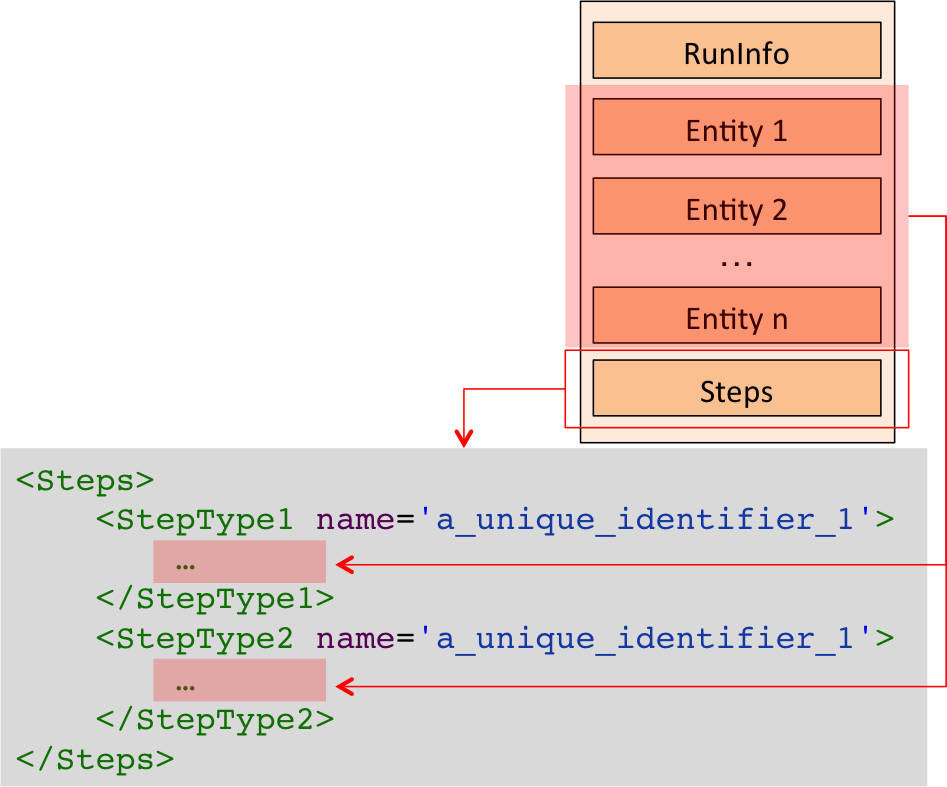
\includegraphics[scale=0.5]{pics/ExampleStepEntity.png}
  \caption{Example of the Steps \textbf{Entity}  and its connection in the input file.}
  \label{fig:ExampleStepEntity}
\end{figure}
  \item \textit{\textbf{Models}}:
  \\ The Models \textbf{Entity}  represents the projection from the input to the output space. Currently, RAVEN defines the
  following sub-categories:
      \begin{itemize}
       \item \textit{Code}, the sub-~\textbf{Entity} that represent the driven code, through external code interfaces (see~\cite{RAVENuserManual})
       \item  \textit{ExternalModel}, the sub-~\textbf{Entity} that represents a physical or mathematical model that is
       directly implemented by the user in a Python module
      \item \textit{ROM}, the sub-~\textbf{Entity} that represent the Reduced Order Model, interfaced with several algorithms
       \item \textit{PostProcessor}, the sub-~\textbf{Entity} that is used to perform action on data, such as computation of
       statistical moments, correlation matrices, etc.
      \end{itemize}
      The Model \textbf{Entity} can be seen as a transfer function between the input and output space.
  \item \textit{\textbf{Functions}}:
   \\ The Functions \textbf{Entity} is the container of all the user-defined functions, such as Goal Functions in adaptive
   sampling strategies, etc.
\end{itemize}
All these action-objects are combined together in order to create a peculiar analysis flow, which is specified
by the user in an additional \textbf{Entity} named \textit{\textbf{Steps}}. This \textbf{Entity} represents the core of the analysis, since it is the location where the multiple objects get finally linked in order to perform a combined action on a certain \textit{Model} (see Fig.~\ref{fig:ExampleStepEntity}). In order to perform this linking, each \textbf{Entity} defined in the Step needs to ``play'' a Role:
\begin{itemize}
  \item \textit{Input}
  \item \textit{Output}
  \item \textit{Model}
  \item \textit{Sampler}
  \item \textit{Function}
  \item \textit{ROM}
  \item \textit{SolutionExport}, the \textbf{Entity} that is used to export the solution of a \textit{Sampler}.
\end{itemize}
Currently, RAVEN supports 4 different types of \textit{\textbf{Steps}}:
\begin{itemize}
  \item \textit{SingleRun}, perform a single run of a model
  \item \textit{MultiRun}, perform multiple runs of a model
  \item \textit{RomTrainer}, perform the training of a Reduced Order Model (ROM)
  \item \textit{PostProcess}, post-process data or manipulate RAVEN entities
  \item \textit{IOStep}, step aimed to perform multiple actions:
  \begin{itemize}
    \item construct/update a Database from a DataObjects and vice-versa
    \item construct/update a Database or a DataObjects object from CSV files
    \item stream the content of a Database or a DataObjects out through an OutStream
    \item store/retrieve a ROM to/from an external File using Pickle module of Python
  \end{itemize}
\end{itemize}

\subsection{Raven Input Structure}
\label{sub:InputStructure}
The RAVEN code does not have a fixed calculation flow, since all of its basic
objects can be combined in order to create a user-defined calculation flow.
%
Thus, its input (XML format) is organized in different XML blocks, each with a
different functionality.
%
The main input blocks are as follows:
\begin{itemize}
  \item \xmlNode{Simulation}: The root node containing the
  entire input, all of
  the following blocks fit inside the \emph{Simulation} block.
  %
  \item \xmlNode{RunInfo}: Specifies the calculation
  settings (number of parallel simulations, etc.).
  %
  \item \xmlNode{Files}: Specifies the files to be
  used in the calculation.
  %
  \item \xmlNode{Distributions}: Defines distributions
  needed for describing parameters, etc.
  %
  \item \xmlNode{Samplers}: Sets up the strategies used for
  exploring an uncertain domain.
  %
  \item \xmlNode{DataObjects}: Specifies internal data objects
  used by RAVEN.
  %
  \item \xmlNode{Databases}: Lists the HDF5 databases used
  as input/output to a
  RAVEN run.
  %
  \item \xmlNode{OutStreams}: Visualization and
  Printing system block.
  %
  \item \xmlNode{Models}: Specifies codes, ROMs,
  post-processing analysis, etc.
  %
  \item \xmlNode{Functions}: Details interfaces to external
  user-defined functions and modules.
  %
  the user will be building and/or running.
  %
  \item \xmlNode{Steps}: Combines other blocks to detail a
  step in the RAVEN workflow including I/O and computations to be performed.
  %
\end{itemize}

Each of these blocks are explained in dedicated sections in the user manual ~\cite{RAVENuserManual}.
%

\input{runInfo.tex}
\input{files.tex}
\input{variablegroups.tex}
\input{ProbabilityDistributions.tex}
\input{sampler.tex}
\input{optimizer.tex}
\section{DataObjects}
\label{sec:DataObjects}

As seen in the previous chapters, different entities in the RAVEN
code interact with each other in order to create, ideally, an infinite number of
different calculation flows.
%
These interactions are made possible through a data handling system that each
entity understands.
%
This system is called the ``DataObjects'' framework.

The \xmlNode{DataObjects} tag is a container of data objects of various types that can
be constructed during the execution of a particular calculation flow.
%
These data objects can be used as input or output for a particular
\textbf{Model} (see Roles' meaning in section \ref{sec:models}), etc.
%
Currently, RAVEN supports 3 different data types, each with a particular
conceptual meaning.
%
These data types are instantiated as sub-nodes in the \xmlNode{DataObjects} block of
an input file:
\begin{itemize}
  \item \xmlNode{PointSet} is a collection of individual objects, each
  describing the state of the system at a certain point (e.g. in time).
  %
  It can be considered a mapping between multiple sets of parameters in the
  input space and the resulting sets of outcomes in the output space at a
  particular point (e.g. in time).
  %
  \item \xmlNode{HistorySet} is a collection of individual objects each
  describing the temporal evolution of the state of the system within a certain
  input domain.
  %
  It can be considered a mapping between multiple sets of parameters in the
  input space and the resulting sets of temporal evolution in the output
  space.
  %
   \item \xmlNode{DataSet} is a generalization of the previously described DataObject,
   aimed to contain a mixture of data (scalars, arrays, etc.). The variables here stored
   can be independent (i.e. scalars) or dependent (arrays) on certain dimensions (e.g. time, coordinates, etc.).
  %
  It can be considered a mapping between multiple sets of parameters in the
  input space (both dependent and/or independent) and the resulting sets of evolution in the output
  space (both dependent and/or independent).
  %
  \nb \textcolor{red} {\textbf{The  \xmlNode{DataSet} is currently usable in the  \xmlNode{EnsembleModel} only (see \ref{subsec:models_EnsembleModel} )}}
\end{itemize}

In summary, the DataObjects accept the following data in their input/output spaces:
\begin{table}[h]
\centering
\caption{DataObjects' accepted data formats.}
\label{DataObjectDataFormatTable}
\begin{tabular}{|c|c|c|}
\hline
\textbf{DataObject}                        & \textbf{Input Space} & \textbf{Output Space} \\ \hline
{\color[HTML]{FE0000} \textit{PointSet}}   & scalars              & scalars               \\ \hline
{\color[HTML]{FE0000} \textit{HistorySet}} & scalars              & vectors               \\ \hline
{\color[HTML]{FE0000} \textit{DataSet}}    & any                  & any                   \\ \hline
\end{tabular}
\end{table}


As noted above, each data object represents a mapping between a set of
parameters and the resulting outcomes.
%
The data objects are defined within the main XML block called \xmlNode{DataObjects}:
\begin{lstlisting}[style=XML]
<Simulation>
   ...
  <DataObjects>
    <PointSet name='***'>...</PointSet>
    <HistorySet name='***'>...</HistorySet>
    <DataSet name='***'>...</DataSet>
  </DataObjects>
   ...
</Simulation>
\end{lstlisting}

Independently on the type of data, the respective XML node has the following
available attributes:
\vspace{-5mm}
\begin{itemize}
  \itemsep0em
  \item \xmlAttr{name}, \xmlDesc{required string attribute}, is a user-defined
  identifier for this data object.
    %
  \nb As with other objects, this name can be used to refer to this specific
  entity from other input blocks in the XML.
  %
%  % Regarding the time attribute, we need to take a better decision... Now it is very confusing.
%  \item \xmlAttr{time}, \xmlDesc{optional float or string attribute}, time
%    attribute.
%    %
%    Here, the user can specify either the time (value) at which the outcomes
%    need to be taken (History-like object, it represents the time from which the
%    outcomes' evolution need to be tracked) or a string  that can be either
%    ``end'', at the end of the history, or ``all'', consider.
%    %
%    \default{random seed};
%  \item \xmlAttr{inputTs}, \xmlDesc{optional integer attribute}, used to
%  specify at which ``time step'' the input space needs to be retrieved.
%  %
%  \nb If the user wants to take conditions from the end of the simulation, s/he
%  can directly input ``-1.''
%  %
%  \default{0}
%  \item \xmlAttr{operator}, \xmlDesc{optional string attribute}, is aimed at
%  performing simple operations on the data to be stored.
%  %
%  %
%  The 3 options currently available are:
%  \begin{itemize}
%    \item \xmlString{max}
%    \item \xmlString{min}
%    \item \xmlString{average}
%  \end{itemize}
%  %
%  \default{None}

  \item \xmlAttr{hierarchical}, \xmlDesc{optional boolean attribute},
  This flag is going to ``control'' the printing/plotting of the DataObject in
  case a hierarchical structure is determined (e.g.
  data coming from Dynamic Event Tree-like approaches):
  \begin{itemize}
    \item if \textbf{True} all the branches of the tree are going to be printed/plotted independently
               (i.e. all the branches are going to be exposed independently)
    \item if \textbf{False} all the branches are going to be walked back and reconstructed in order to create independent histories
  \end{itemize}
  %
  \default{False}
\end{itemize}
\vspace{-5mm}
In each XML node (e.g. \xmlNode{PointSet}, \xmlNode{HistorySet} or  \xmlNode{DataSet}), the user
specifies the following sub-nodes:
\begin{itemize}
  \item \xmlNode{Input}, \xmlDesc{comma separated string, required field}, lists
  the input parameters to which this data is connected.
  %
  \item \xmlNode{Output}, \xmlDesc{comma separated string, required field}, lists
  the output parameters to which this data is connected.
  %
  \item \xmlNode{Index}, \xmlDesc{comma separated string, required for \xmlNode{DataSet}}, lists
  the dependent variables that depend on this index (specified through the attribute  \xmlAttr{var}).
  This XML node requires the following attribute:
   \begin{itemize}
     \item \xmlAttr{var}, \xmlDesc{required string attribute}, the dimension name of this index (e.g. time)
   \end{itemize}
 \item \xmlNode{options}, \xmlDesc{optional node}, contains additional option nodes
   for data objects.  This node contains the following subnodes:
   \begin{itemize}
     \item \xmlNode{pivotParameter}, \xmlDesc{optional, string}, specifies the \textit{pivotParameter} for a
       \xmlNode{HistorySet}. The pivot parameter is the shared index of the output variables in the data
       object.  \default time
    \item \xmlNode{inputRow}, \xmlDesc{integer, optional field}, used to
         specify  the row (in a CSV file or HDF5 table) from which the input space
        needs to be retrieved (e.g. the time-step);
    %
    \item \xmlNode{outputRow}, \xmlDesc{integer, optional field}, used to
         specify  the row (in the CSV file or HDF5 table) from which the output space
        needs to be retrieved (e.g. the time-step). If this node is inputted, the nodes
         \xmlNode{operator} and  \xmlNode{outputPivotValue} can not be inputted (mutually exclusive).
       \\\nb This XML node is available for DataObjects of type \xmlNode{PointSet} only;
    %
    \item \xmlNode{operator}, \xmlDesc{string, optional field}, is aimed to perform
         simple operations on the data to be stored.
         The 3 options currently available are:
         \begin{itemize}
            \item \xmlString{max}
            \item \xmlString{min}
            \item \xmlString{average}
         \end{itemize}
         If this node is inputted, the nodes
         \xmlNode{outputRow} and  \xmlNode{outputPivotValue} can not be inputted (mutually exclusive).
         \\\nb This XML node is available for DataObjects of type \xmlNode{PointSet} only;
   \end{itemize}

  %
\end{itemize}

The  \xmlNode{PointSet} and  \xmlNode{HistorySet} objects are a specialization of the  \xmlNode{DataSet}. In
the \xmlNode{PointSet}, the input and output space are all exclusively scalar values.  These values might be
extracted from a vector of values for each entry using the \xmlNode{options} node, but the end result is a
single scalar per input or output variable.

For the \xmlNode{HistorySet}, all inputs must be scalar, and all outputs must share an index (the
\textit{pivotParameter}.  There cannot be scalars in any of the outputs. The pivotParameter can be changed
through the corresponding node in the \xmlNode{options} node.


  %
  %%%%%%%%%%%%%%%%%%%%%%%%%%%%%%%%%%%%%%%%%%%%%%%%%%%%%%%%%%%%%%%%%%%%%%%%%%%%%%
  %%%% This feature is being disabled until the DataObjects handle data in a
  %%%% more encapsulated fashion. When the data can handle this all internally
  %%%% then we can re-add this feature. As of now, determining the rows
  %%%% associated to the outputPivotValue or inputPivotValue requires knowing
  %%%% information outside of the "value" passed into
  %%%% DataObject.updateOutputValue or DataObject.updateInputValue, thus the
  %%%% caller has to do this computation, but currently the caller occurs in ~50
  %%%% different places according to my grep of "updateOutputValue"
  %%%% -- DPM 8/29/2017
  % \item \xmlNode{pivotParameter}, \xmlDesc{string, optional field} the name of
  %   the parameter whose values need to be used as reference for the values
  %   specified in the XML nodes \xmlNode{inputPivotValue},
  %   \xmlNode{outputPivotValue}, or \xmlNode{inputPivotValue} (if inputted).
  %   This field can be used, for example, if the driven code output file uses  a
  %   different name for the variable ``time'' or to specify a different reference
  %   parameter (e.g. PRESSURE). Default value is \xmlString{time}.
  %   \\\nb The variable specified here should be monotonic; the code does not
  %   check for eventual oscillation and is going to take the first occurance for
  %   the values specified in the XML nodes \xmlNode{inputPivotValue},
  %   \xmlNode{outputPivotValue}, and  \xmlNode{inputPivotValue};
  % %
  % \item \xmlNode{inputPivotValue}, \xmlDesc{float, optional field}, the value of the \xmlNode{pivotParameter} at which the input space needs to be retrieved
  %   If this node is inputted, the node  \xmlNode{inputRow} can not be inputted (mutually exclusive).
  %   %
  % \item \xmlNode{outputPivotValue}. This node can be either a float or a list of floats, depending on the type of DataObjects:
  %  \begin{itemize}
  %     \item if \xmlNode{HistorySet},\xmlNode{outputPivotValue}, \xmlDesc{list of floats, optional field},  list of values of the
  %                         \xmlNode{pivotParameter} at which the output space needs to be retrieved;
  %     \item if \xmlNode{PointSet},\xmlNode{outputPivotValue}, \xmlDesc{float, optional field},  the value of the \xmlNode{pivotParameter}
  %        at which the output space needs to be retrieved. If this node is inputted, the node  \xmlNode{outputRow} can not be inputted (mutually exclusive);
  %  \end{itemize}
  %%%%%%%%%%%%%%%%%%%%%%%%%%%%%%%%%%%%%%%%%%%%%%%%%%%%%%%%%%%%%%%%%%%%%%%%%%%%%%
  %
Note that if the optional nodes in the block \xmlNode{options} are not inputted, the following default are applied:
\begin{itemize}
   \item the Input space (scalars) is retrieved from the first row in the CSVs files or HDF5 tables (if the parameters specified are not
      among the variables sampled by RAVEN); In case of the  \xmlNode{DataSet}, if any of the input space variables depend on an \xmlNode{Index}, they
      are going to be linked to the \xmlNode{Index} variable
   \item  the output space defaults are as follows:
   \begin{itemize}
       \item if \xmlNode{PointSet}, the output space is retrieved from the last row in the CSVs files or HDF5 tables;
       \item if \xmlNode{HistorySet}, the output space is represented by all the rows found in  the CSVs or HDF5 tables.
       \item if \xmlNode{DataSet}, the output space of the variables that do not depends on any index is retrieved from the last row in the CSVs files or HDF5 tables;
       on the contrary, the output space of the variables that depends on indexes is represented by all the rows found in  the CSVs or HDF5 tables (if they match
       with the indexes' dimension)
    \end{itemize}
\end{itemize}


\begin{lstlisting}[style=XML,morekeywords={operator,hierarchical,name,var}]
  <DataObjects>
    <PointSet name='outTPS1'>
      <options>
       <inputRow>1</inputRow>
       <outputRow>-1</outputRow>
      </options>
      <Input>pipe_Area,pipe_Dh,Dummy1</Input>
      <Output>pipe_Hw,pipe_Tw,time</Output>
    </PointSet>
    <HistorySet name='stories1'>
        <options>
            <pivotParameter>TIME</pivotParameter>
            <inputRow>1</inputRow>
            <outputRow>-1</outputRow>
        </options>
      <Input>pipe_Area,pipe_Dh</Input>
      <Output>pipe_Hw,pipe_Tw,time</Output>
    </HistorySet>
    <DataSet name='aDataSet'>
      <Input>pipe_Area,pipe_Dh</Input>
      <Output>pipe_Hw,pipe_Tw</Output>
      <Index var="time">pipe_Hw,pipe_Tw</Index>
    </DataSet>
  </DataObjects>
\end{lstlisting}

\section{Databases}
\label{sec:Databases}
The RAVEN framework provides the capability to store and retrieve data to/from
an external database.
%
Currently RAVEN has support for only a database type called \textbf{HDF5}.
%
This database, depending on the data format it is receiving, will organize
itself in a ``parallel'' or ``hierarchical'' fashion.
%
The user can create as many database objects as needed.
%
The Database objects are defined within the main XML block called
\xmlNode{Databases}:
\begin{lstlisting}[style=XML]
<Simulation>
  ...
  <Databases>
    ...
    <HDF5 name="aDatabaseName1" readMode="overwrite"/>
    <HDF5 name="aDatabaseName2" readMode="overwrite"/>
    ...
  </Databases>
  ...
</Simulation>
\end{lstlisting}
The specifications of each Database of type HDF5 needs to be defined within the
XML block \xmlNode{HDF5}, that recognizes the following attributes:
\vspace{-5mm}
\begin{itemize}
  \itemsep0em
  \item \xmlAttr{name}, \xmlDesc{required string attribute}, a user-defined
  identifier of this object.
  %
  \nb As with other objects, this is name can be used to reference this specific
  entity from other input blocks in the XML.
  \item \xmlAttr{readMode}, \xmlDesc{required string attribute}, defines whether an existing database should
    be read when loaded (\xmlString{read}) or overwritten (\xmlString{overwrite}).
    \nb if in \xmlString{read} mode and the database is not found, RAVEN will read in
    the data as empty and raise a warning, NOT an error.
  %
  \item \xmlAttr{directory}, \xmlDesc{optional string attribute}, this attribute
  can be used to specify a particular directory path where the database will be
  created or read from.  If an absolute path is given, RAVEN will respect it; otherwise,
  the path will be assumed to be relative to the \xmlNode{WorkingDir} from the \xmlNode{RunInfo} block.
  RAVEN recognizes path expansion tools such as tildes (\emph{user dir}), single dots (\emph{current dir}),
  and double dots (\emph{parent dir}).
  %
  \default{workingDir/DatabaseStorage}.  The \xmlNode{workingDir} is
   the one defined within the \xmlNode{RunInfo} XML block (see Section~\ref{sec:RunInfo}).
  \item \xmlAttr{filename}, \xmlDesc{optional string attribute}, specifies the
  filename of the HDF5 that will be created in the \xmlAttr{directory}.
  %
  \nb When this attribute is not specified, the newer database filename will be
  named \texttt{name}.h5, where \textit{name} corresponds to the \xmlAttr{name}
  attribute of this object.
  %
  \default{None}
  \item \xmlAttr{compression}, \xmlDesc{optional string attribute}, compression
  algorithm to be used.
  %
  Available are:
  \begin{itemize}
    \item \xmlString{gzip}, best where portability is required.
    %
    Good compression, moderate speed.
    %
    \item \xmlString{lzf}, Low to moderate compression, very fast.
    %
  \end{itemize}
  \default{None}
\end{itemize}

In addition, the \xmlNode{HDF5} recognizes the following subnodes:
\begin{itemize}
  \itemsep0em
  \item \xmlNode{variables}, \xmlDesc{optional, comma-separated string}, allows only a pre-specified set of variables to be
    included in the HDF5 when it is written to.  If this node is not included, by default the HDF5 will
    include ALL of the input/output variables as a result of the step it is part of.  If included, only the
    comma-separated variable names will be included if found.

    \nb RAVEN will not error if one of the requested variables is not found; instead, it will silently pass.
    It is recommended that a small trial run is performed, loading the HDF5 back into a data object, to check
    that the correct variables are saved to the HDF5 before performing large-scale calculations.
\end{itemize}


Example:
\begin{lstlisting}[style=XML,morekeywords={directory,filename}]
<Databases>
  <HDF5 name="aDatabaseName1" directory=''path_to_a_dir'' compression=''lzf'' readMode='overwrite'/>
  <HDF5 name="aDatabaseName2" filename=''aDatabaseName2.h5'' readMode='read'/>
</Databases>
\end{lstlisting}

\input{OutStreamSystem.tex}
\input{model.tex}
\input{functions.tex}

\section{Metrics}
\label{sec:Metrics}

\newcommand{\metrictypeI}[3]
{
  This metric interface directly with the metric available within \textit{#1}.
  The specifications of this metric must be defined within the XML block \xmlNode{#2}.
  This XML node needs to contain the following subnode:

  \begin{itemize}
    \item \xmlNode{metricType}\texttt{#3}\xmlNode{/metricType}, \xmlDesc{vertical bar (\texttt{|}) separated
      string, required field}.
  \end{itemize}

}
\newcommand{\metrictypeII}[3]
{
  \metrictypeI{#1}{#2}{#3}

  In addition to this XML subnode, the users can also specify the weights for given metric:
  \begin{itemize}
    \item \xmlNode{w}, \xmlDesc{comma separated floats, optional parameter}, the weights for each value in \textit{u}
      and \textit{v}. Default is None, which gives each value a weight of 1.0.
  \end{itemize}
}

\newcommand{\metrictypeIII}[3]
{
  \metrictypeI{#1}{#2}{#3}

  In addition to this XML subnode, the users can also specify the weights for given metric:
  \begin{itemize}
    \item \xmlNode{sample\_weight}, \xmlDesc{comma separated floats, optional parameter}, the weights for each value in \textit{u}
      and \textit{v}. Default is None, which gives each value a weight of 1.0.
  \end{itemize}
}

The Metrics block allows the user to specify the similarity/dissimilarity metrics to be used for other
RAVEN entities, such as \textbf{PostProcessors}, and \textbf{HybridModel}.

In the RAVEN input file these metrics are defined as follows:
\begin{lstlisting}[style=XML]
<Simulation>
  ...
  <Metrics>
    ...
    <MetricID name='metricName'>
      ...
     <param1>value</param1>
      ...
    </MetricID>
    ...
  </Metrics>
  ...
</Simulation>
\end{lstlisting}

The metrics, that are available in RAVEN, can be categorized into several main classes:
\begin{itemize}
  \item \textbf{Paired Distance Metric}, distance metrics between two variables $u$ and $v$, such as \xmlString{euclidean},
    \xmlString{manhattan}, \xmlString{minkowski} and so on.
  \item \textbf{Regression Metric}, measure the regression performance, such as \xmlString{mean\_squared\_error},
    \xmlString{r2\_score}, \xmlString{explained\_variance\_score} and \xmlString{mean\_absolute\_error}.
  \item \textbf{Boolean Metric}, distance metrics between two boolean variables $u$ and $v$, such as
    \xmlString{dice}, \xmlString{hamming}, \xmlString{yule} and so on.
  \item \textbf{Pairwise Metric}, compute the distance or kernel between each pair of the two collections of input
    or observations in n-dimensional space.
    \nb These metrics can be only used in the clustering post-processor of data mining. 
  \item \textbf{Other metric}, such as \xmlString{DTW}.
\end{itemize}

The valid \textbf{MetricID}s are: \xmlNode{SKL}, \xmlNode{ScipyMetric}, \xmlNode{DTW}, \xmlNode{CDFAreaDifference},
and \xmlNode{PDFCommonArea}. This XML node requires the following attributes:
\begin{itemize}
  \item \xmlAttr{name}, \xmlDesc{required string attribute}, user-defined name of this metric. \nb As with other
    objects, this name can be used to refer to this specific entity from other input blocks in the XML.
\end{itemize}

\nb If you are using \xmlNode{ScipyMetric}, please pay more attention on the weight associated with the metric
calculations. Scipy does not normalize the weight during the calculation, and the results can be significant difference
from the normalized weight.

In RAVEN, lots of metrics are just interfaces directly with metrics available within \textbf{Scipy} and
\textbf{SciKit-Learn}. In this case, the algorithm for the metrics is choosen by the subnode \xmlNode{metricType}
under the parent node \xmlNode{SKL} (metric from SciKit-Learn) or \xmlNode{ScipyMetric} (metric from Scipy). For
example, \xmlNode{metricType}\xmlString{paired\_distance|euclidean}\xmlNode{/metricType}.

In the following sub-sections, the input requirements for all of the metrics are presented in the following sections.

%%%%%%%%%%%%%%%%%%%%%%%%%%%%%%%%%%%%%%%%%%%%%%%%%%%%%%%%%%%%%%%%%%%%%%%%%%%%%%%%%%%%%%%%%%%%%%%%%%%
% paired_distance metric
%%%%%%%%%%%%%%%%%%%%%%%%%%%%%%%%%%%%%%%%%%%%%%%%%%%%%%%%%%%%%%%%%%%%%%%%%%%%%%%%%%%%%%%%%%%%%%%%%%%
\subsection{Paired Distance Metric}
\label{subsection:pairedDistance}

\subsubsection{Euclidean}
This metric compute the paired euclidean distances between $u$ and $v$, i.e.
\begin{equation}
  {||u-v||}_2
\end{equation}

\metrictypeI{SciKit-Learn}{SKL}{paired\_distance|euclidean}

\subsubsection{Cosine}
This metric computes the paired cosine distances between $u$ and $v$, i.e.
\begin{equation}
  1 - \frac{u \cdot v}{||u||_2 ||v||_2}
\end{equation}
where $u \cdot v$ is the dot product of $u$ and $v$

\metrictypeI{SciKit-Learn}{SKL}{paired\_distance|cosine}

\subsubsection{Manhattan}
This metric computes the L1 distances between $u$ and $v$, i.e.
\begin{equation}
  \sum_i {\left| u_i - v_i \right|}
\end{equation}

\metrictypeI{SciKit-Learn}{SKL}{paired\_distance|manhattan}

\subsubsection{Braycurtis}
This metric computes the Bray-Curtis distances between $u$ and $v$, i.e.
\begin{equation}
  \sum{|u_i-v_i|} / \sum{|u_i+v_i|}
\end{equation}
The Bray-Curtis distance is in the range $[0, 1]$.
\metrictypeII{Scipy}{ScipyMetric}{paired\_distance|braycurtis}

\subsubsection{Canberra}
This metric computes the Canberra distance between $u$ and $v$, i.e.
\begin{equation}
  d(u,v) = \sum_i \frac{|u_i-v_i|}{|u_i|+|v_i|}
\end{equation}

\metrictypeII{Scipy}{ScipyMetric}{paired\_distance|canberra}

\subsubsection{Correlation}
This metric computes the correlation distance between $u$ and $v$, i.e.
\begin{equation}
  1 - \frac{(u - \bar{u}) \cdot (v - \bar{v})}{{||(u - \bar{u})||}_2 {||(v - \bar{v})||}_2}
\end{equation}
where $\bar{u}$ is the mean of the elements of $u$

\metrictypeII{Scipy}{ScipyMetric}{paired\_distance|correlation}

\subsubsection{Minkowski}
This metric computes the Minkowski distance between $u$ and $v$, i.e.
\begin{equation}
  {||u-v||}_p = (\sum{|u_i - v_i|^p})^{1/p}
\end{equation}

\metrictypeII{Scipy}{ScipyMetric}{paired\_distance|minkowski}

\begin{itemize}
  \item \xmlNode{p}, \xmlDesc{float, required field}, value for the parameter $p$
\end{itemize}

In the RAVEN input file, these metrics are defined as follows:
\begin{lstlisting}[style=XML]
<Simulation>
  ...
  <Metrics>
    <SKL name="euclidean">
        <metricType>paired_distance|euclidean</metricType>
    </SKL>
    <SKL name="cosine">
        <metricType>paired_distance|cosine</metricType>
    </SKL>
    <SKL name="manhattan">
        <metricType>paired_distance|manhattan</metricType>
    </SKL>
    <ScipyMetric name="braycurtis">
      <metricType>paired_distance|braycurtis</metricType>
    </ScipyMetric>
    <ScipyMetric name="canberra">
        <metricType>paired_distance|canberra</metricType>
    </ScipyMetric>
    <ScipyMetric name="correlation">
        <metricType>paired_distance|correlation</metricType>
    </ScipyMetric>
    <ScipyMetric name="minkowski">
        <metricType>paired_distance|minkowski</metricType>
        <p>5</p>
        <w>0.1, 0.1, 0.1, 0.1, 0.1</w>
    </ScipyMetric>
  </Metrics>
  ...
</Simulation>
\end{lstlisting}

%%%%%%%%%%%%%%%%%%%%%%%%%%%%%%%%%%%%%%%%%%%%%%%%%%%%%%%%%%%%%%%%%%%%%%%%%%%%%%%%%%%%%%%%%%%%%%%%%%%
% regression  metric
%%%%%%%%%%%%%%%%%%%%%%%%%%%%%%%%%%%%%%%%%%%%%%%%%%%%%%%%%%%%%%%%%%%%%%%%%%%%%%%%%%%%%%%%%%%%%%%%%%%
\subsection{Regression Metric}
\label{subsection:regression}

\subsubsection{Explained variance score}
This metric computes the explained variance regression score, i.e.
\begin{equation}
  1.0 - \frac{Var[u-v]}{Var[u]}
\end{equation}
The best possible score is 1.0, lower values are worse.

\metrictypeIII{Scikit-Learn}{SKL}{regression|explained\_variance\_score}

\subsubsection{Mean absolute error}
This metric computes mean absolute error, a risk metric corresponding to the expected value of the absolute
error loss or \textit{l1}-norm loss.
\begin{equation}
  \frac{1}{n_{samples}}\sum_{i=0}^{n_{samples}-1}|u_i-v_i|
\end{equation}

\metrictypeIII{Scikit-Learn}{SKL}{regression|mean\_absolute\_error}

\subsubsection{Mean squared error}
This metric computes mean square error, a risk metric corresponding to the expected value of the
squared error or loss.
\begin{equation}
  \frac{1}{n_{samples}}\sum_{i=0}^{n_{samples}-1}(u_i-v_i)^2
\end{equation}

\metrictypeIII{Scikit-Learn}{SKL}{regression|mean\_squared\_error}

\subsubsection{R2 score}
This metric computes the coefficient of determination, i.e.
\begin{equation}
  1.0-\frac{\sum_{i=0}^{n_{samples}-1}(u_i-v_i)^2}{\sum_{i=0}^{n_{samples}-1}(u_i-mean[u])^2}
\end{equation}
It provides a measure of how well future samples are likely to be predicted by the model.
Best possible score is 1.0 and it can be negative.

\metrictypeIII{Scikit-Learn}{SKL}{regression|r2\_score}

In the RAVEN input file, these metrics are defined as follows:
\begin{lstlisting}[style=XML]
<Simulation>
  ...
  <Metrics>
    <SKL name="explained_variance_score">
        <metricType>regression|explained_variance_score</metricType>
        <sample_weight>0.1,0.1,0.1,0.05,0.05</sample_weight>
    </SKL>
    <SKL name="mean_absolute_error">
        <metricType>regression|mean_absolute_error</metricType>
        <sample_weight>0.1,0.1,0.1,0.05,0.05</sample_weight>
    </SKL>
    <SKL name="r2_score">
        <metricType>regression|r2_score</metricType>
        <sample_weight>0.1,0.1,0.1,0.05,0.05</sample_weight>
    </SKL>
    <SKL name="mean_squared_error">
        <metricType>regression|mean_squared_error</metricType>
        <sample_weight>0.1,0.1,0.1,0.05,0.05</sample_weight>
    </SKL>
  </Metrics>
  ...
</Simulation>
\end{lstlisting}

%%%%%%%%%%%%%%%%%%%%%%%%%%%%%%%%%%%%%%%%%%%%%%%%%%%%%%%%%%%%%%%%%%%%%%%%%%%%%%%%%%%%%%%%%%%%%%%%%%%
% boolean  metric
%%%%%%%%%%%%%%%%%%%%%%%%%%%%%%%%%%%%%%%%%%%%%%%%%%%%%%%%%%%%%%%%%%%%%%%%%%%%%%%%%%%%%%%%%%%%%%%%%%%
\subsection{Boolean Metric}
\label{subsection:boolean}

\subsubsection{Dice}
This metric computes the Dice dissimilarity between two boolean variables $u$ and $v$
\begin{equation}
  \frac{c_{TF} + c_{FT}}{2c_{TT} + c_{FT} + c_{TF}}
\end{equation}
where $c_{ij}$ is the number of occurrences of $\mathtt{u[k]} = i$ and $\mathtt{v[k]} = j$ for $k < n$

\metrictypeII{Scipy}{ScipyMetric}{boolean|dice}

\subsubsection{Hamming}
This metric computes the Hamming distance between two boolean variables $u$ and $v$, i.e.
\begin{equation}
  \frac{c_{01} + c_{10}}{n}
\end{equation}
where $c_{ij}$ is the number of occurrences of $\mathtt{u[k]} = i$ and $\mathtt{v[k]} = j$ for $k < n$

\metrictypeII{Scipy}{ScipyMetric}{boolean|hamming}

\subsubsection{Jaccard}
This metric computes the Jaccard-Needham dissimilarity distance between two boolean variables $u$ and $v$, i.e.
\begin{equation}
  \frac{c_{TF} + c_{FT}}{c_{TT} + c_{FT} + c_{TF}}
\end{equation}
where $c_{ij}$ is the number of occurrences of $\mathtt{u[k]} = i$ and $\mathtt{v[k]} = j$ for $k < n$

\metrictypeII{Scipy}{ScipyMetric}{boolean|jaccard}

\subsubsection{Kulsinski}
This metric computes the Kulsinski dissimilarity distance between two boolean variables $u$ and $v$, i.e.
\begin{equation}
  \frac{c_{TF} + c_{FT} - c_{TT} + n}{c_{FT} + c_{TF} + n}
\end{equation}
where $c_{ij}$ is the number of occurrences of $\mathtt{u[k]} = i$ and $\mathtt{v[k]} = j$ for $k < n$

\metrictypeII{Scipy}{ScipyMetric}{boolean|kulsinski}

\subsubsection{Rogerstanimoto}
This metric computes the Rogers-Tanimoto dissimilarity distance between two boolean variables $u$ and $v$, i.e.
\begin{equation}
  \frac{R}{c_{TT} + c_{FF} + R}
\end{equation}
where $c_{ij}$ is the number of occurrences of $\mathtt{u[k]} = i$ and $\mathtt{v[k]} = j$
for $k < n$ and $R = 2(c_{TF} + c_{FT})$

\metrictypeII{Scipy}{ScipyMetric}{boolean|rogerstanimoto}

\subsubsection{Russellrao}
This metric computes the Russell-Rao dissimilarity distance between two boolean variables $u$ and $v$, i.e.
\begin{equation}
  \frac{n - c_{TT}}{n}
\end{equation}
where $c_{ij}$ is the number of occurrences of $\mathtt{u[k]} = i$ and $\mathtt{v[k]} = j$ for $k < n$

\metrictypeII{Scipy}{ScipyMetric}{boolean|russellrao}

\subsubsection{Sokalmichener}
This metric computes the Sokal-Michener dissimilarity distance between two boolean variables $u$ and $v$, i.e.
\begin{equation}
  \frac{R}{S + R}
\end{equation}
where $c_{ij}$ is the number of occurrences of $\mathtt{u[k]} = i$ and $\mathtt{v[k]} = j$ for
$k < n$, $R = 2 * (c_{TF} + c_{FT})$ and $S = c_{FF} + c_{TT}$

\metrictypeII{Scipy}{ScipyMetric}{boolean|sokalmichener}

\subsubsection{Sokalsneath}
This metric computes the Sokal-Sneath dissimilarity distance between two boolean variables $u$ and $v$, i.e.
\begin{equation}
  \frac{R}{c_{TT} + R}
\end{equation}
where $c_{ij}$ is the number of occurrences of $\mathtt{u[k]} = i$ and $\mathtt{v[k]} = j$
for $k < n$ and $R = 2(c_{TF} + c_{FT})$

\metrictypeII{Scipy}{ScipyMetric}{boolean|sokalsneath}

\subsubsection{Yule}
This metric computes the Yule dissimilarity distance between two boolean variables $u$ and $v$, i.e.
\begin{equation}
  \frac{R}{c_{TT} * c_{FF} + \frac{R}{2}}
\end{equation}
where $c_{ij}$ is the number of occurrences of $\mathtt{u[k]} = i$ and $\mathtt{v[k]} = j$ for
$k < n$ and $R = 2.0 * c_{TF} * c_{FT}$

\metrictypeII{Scipy}{ScipyMetric}{boolean|yule}

% TODO: the following metrics require different function interfaces
%  \item From scipy.spatial.distance
%       and $x \cdot y$ is the dot product of $x$ and $y$
%       \item mahalanobis: $\sqrt{ (u-v) V^{-1} (u-v)^T }$ where $V$ is the covariance matrix.  Note that the argument $VI$ is the inverse of $V$
%       \item seuclidean: $\sqrt{\sum {(u_i-v_i)^2 / V[x_i]}}$ where $V$ is the variance vector; $V[i]$ is the variance computed over all the i'th components of the points.
%        If not passed, it is automatically computed.
%       \item sqeuclidean: ${||u-v||}_2^2$

An example of Boolean metric defined in RAVEN is provided below:
\begin{lstlisting}[style=XML]
<Simulation>
  ...
  <Metrics>
    ...
    <ScipyMetric name="rogerstanimoto">
        <metricType>boolean|rogerstanimoto</metricType>
    </ScipyMetric>
    <ScipyMetric name="dice">
        <metricType>boolean|dice</metricType>
    </ScipyMetric>
    <ScipyMetric name="hamming">
        <metricType>boolean|hamming</metricType>
    </ScipyMetric>
    <ScipyMetric name="jaccard">
        <metricType>boolean|jaccard</metricType>
    </ScipyMetric>
    <ScipyMetric name="kulsinski">
        <metricType>boolean|kulsinski</metricType>
    </ScipyMetric>
    <ScipyMetric name="russellrao">
        <metricType>boolean|russellrao</metricType>
    </ScipyMetric>
    <ScipyMetric name="sokalmichener">
        <metricType>boolean|sokalmichener</metricType>
    </ScipyMetric>
    <ScipyMetric name="sokalsneath">
        <metricType>boolean|sokalsneath</metricType>
    </ScipyMetric>
    <ScipyMetric name="yule">
        <metricType>boolean|yule</metricType>
    </ScipyMetric>
    ...
  </Metrics>
  ...
</Simulation>
\end{lstlisting}

%%%%%%%%%%%%%%%%%%%%%%%%%%%%%%%%%%%%%%%%%%%%%%%%%%%%%%%%%%%%%%%%%%%%%%%%%%%%%%%%%%%%%%%%%%%
\subsection{Dynamic Time Warping}
\label{subsection:DTW}
The Dynamic Time Warping (DTW) is a distance metrice that is used to measure similarity
between two sequences, i.e. temporal sequences.

The specifications of a DTW distance must be defined within the XML block.
\xmlNode{DTW}.

This XML node needs to contain the attributes:


\begin{itemize}
  \item \xmlNode{order},          \xmlDesc{int, required field},    order of the DTW calculation: $0$ specifices a classical DTW caluclation and $1$ specifies
                                                                    a derivative DTW calculation
  \item \xmlNode{localDistance},  \xmlDesc{string, required field}, the ID of the distance function to be employed to determine the local distance
                                                                    evaluation of two time series. Available options are provided by the Scipy
                                                                    pairwise distances (cityblock, cosine, euclidean, $l1$, $l2$, manhattan,
                                                                    braycurtis, canberra, chebyshev, correlation, dice, hamming, jaccard,
                                                                    kulsinski, mahalanobis, matching, minkowski, rogerstanimoto, russellrao,
                                                                    seuclidean, sokalmichener, sokalsneath, sqeuclidean, yule)
\end{itemize}

An example of Minkowski distance defined in RAVEN is provided below:
\begin{lstlisting}[style=XML]
<Simulation>
  ...
  <Metrics>
    ...
    <DTW name="example">
      <order>0</order>
      <localDistance>euclidean</localDistance>
    </DTW>
    ...
  </Metrics>
  ...
</Simulation>
\end{lstlisting}

%%%%%%%%%%%%%%%%%%%%%%%%%%%%%%%%%%%%%%%%%%%%%%%%%%%%%%%%%%%%%%%%%%%%%%%%%%%%%%%%%%%%%%%%
\subsection{CDFAreaDifference}

This calculates the difference in area between the two CDFs.  This
metric supports using distributions as input.  Other inputs are
converted to a CDF.

\begin{equation}
  \text{CDF area difference} = \int_{-\infty}^{\infty}{\|CDF_a(x)-CDF_b(x)\|dx}
\end{equation}

This metric has the same units as $x$.  The closer the number is
to zero, the closer the match.  A perfect match would be 0.0.

An example is provided below:
\begin{lstlisting}[style=XML]
<Simulation>
  ...
  <Metrics>
    ...
    <CDFAreaDifference name="cdf_diff" />
    ...
  </Metrics>
  ...
</Simulation>
\end{lstlisting}

%%%%%%%%%%%%%%%%%%%%%%%%%%%%%%%%%%%%%%%%%%%%%%%%%%%%%%%%%%%%%%%%%%%%%%%%%%%%%%%%%%%%%%%%
\subsection{PDFCommonArea}

This calculates the common area between the two PDFs.  The higher the
value the closer the PDFs are.  This metric supports distributions as
inputs.  Other inputs are converted to a PDF.

\begin{equation}
  \text{PDF common area} = \int_{-\infty}^{\infty}{\min(PDF_a(x),PDF_b(x))}dx
\end{equation}

A perfect match would be 1.0.


An example is provided below:
\begin{lstlisting}[style=XML]
<Simulation>
  ...
  <Metrics>
    ...
    <PDFCommonArea name="pdf_area" />
    ...
  </Metrics>
  ...
</Simulation>
\end{lstlisting}

%%%%%%%%%%%%%%%%%%%%%%%%%%%%%%%%%%%%%%%%%%%%%%%%%%%%%%%%%%%%%%%%%%%%%%%%%%%%%%%%%%%%%%%%%%%%%%%%%%%
% Pairwise metric
%%%%%%%%%%%%%%%%%%%%%%%%%%%%%%%%%%%%%%%%%%%%%%%%%%%%%%%%%%%%%%%%%%%%%%%%%%%%%%%%%%%%%%%%%%%%%%%%%%%
\subsection{Pairwise Metric}
\label{subsection:pairwiseMetric}
This calculates the pairwise distance or kernel between each row of the two collections of inputs. This
metric can be only used in the \textbf{DataMining} post-processor.

\subsubsection{Polynomial}
Compute the polynomial kernel between $X$ and $Y$:
\begin{equation}
  K(X, Y) = (gamma <X, Y> + coef0)^{degree}
\end{equation}
\metrictypeI{Scikit-Learn}{PairwiseMetric}{kernel|Polynomial}
In addition to this XML subnode, the users can also specify the following subnodes:
\begin{itemize}
  \item \xmlNode{degree}, \xmlDesc{integer, optional parameter}, default `3'
  \item \xmlNode{gamma}, \xmlDesc{float, optional parameter}, default $1.0/numberColumnsInX$
  \item \xmlNode{coef0}, \xmlDesc{integer, optional parameter}, default `1'
\end{itemize}

\subsubsection{additive\_chi2}
Computes the additive chi-squared kernel between observations in $X$ and $Y$
The chi-squared kernel is computed between each pair of rows in $X$ and $Y$. $X$ and $Y$ have to be non-negative.
This kernel is most commonly applied to histograms.
The chi-squared kernel is given by:
\begin{equation}
  K(x, y) = - Sum [(x - y)^2 / (x + y)]
\end{equation}

\metrictypeI{Scikit-Learn}{PairwiseMetric}{kernel|additive\_chi2}

\subsubsection{chi2}
Computes the exponential chi-squared kernel between observations in $X$ and $Y$
The chi-squared kernel is computed between each pair of rows in $X$ and $Y$. $X$ and $Y$ have to be non-negative.
This kernel is most commonly applied to histograms.
The chi-squared kernel is given by:
\begin{equation}
  K(x, y) = exp(- gamma * Sum [(x - y)^2 / (x + y)])
\end{equation}

\metrictypeI{Scikit-Learn}{PairwiseMetric}{kernel|chi2}
In addition to this XML subnode, the users can also specify the following subnodes:
\begin{itemize}
  \item \xmlNode{gamma}, \xmlDesc{float, optional parameter}, default `1' 
\end{itemize}

\subsubsection{cosine\_similarity}
Compute the cosine similarity between $X$ and $Y$:
\begin{equation}
  K(X, Y) = <X, Y> / (||X||*||Y||)
\end{equation}

\metrictypeI{Scikit-Learn}{PairwiseMetric}{kernel|cosine\_similarity}

\subsubsection{laplacian}
Computes the laplacian kernel between observations in $X$ and $Y$
The laplacian kernel is given by:
\begin{equation}
  K(x, y) = exp(- gamma * ||x - y||_1)
\end{equation}
for each pair of rows $x$ in $X$ and $y$ in $Y$.
\metrictypeI{Scikit-Learn}{PairwiseMetric}{kernel|laplacian}
In addition to this XML subnode, the users can also specify the following subnodes:
\begin{itemize}
  \item \xmlNode{gamma}, \xmlDesc{float, optional parameter}, default $1.0/numberColumnsInX$
\end{itemize}

\subsubsection{linear}
computes the linear kernel between $X$ and $Y$
\begin{equation}
  K(X, Y) = X^T * Y
\end{equation}
\metrictypeI{Scikit-Learn}{PairwiseMetric}{kernel|linear}

\subsubsection{rbf}
Computes the laplacian kernel between observations in $X$ and $Y$
The laplacian kernel is given by:
\begin{equation}
  K(x, y) = exp(- gamma * ||x - y||^2)
\end{equation}
for each pair of rows $x$ in $X$ and $y$ in $Y$.
\metrictypeI{Scikit-Learn}{PairwiseMetric}{kernel|rbf}
\begin{itemize}
  \item \xmlNode{gamma}, \xmlDesc{float, optional parameter}, default $1.0/numberColumnsInX$
\end{itemize}

\subsubsection{sigmoid}
Compute the sigmoid kernel between $X$ and $Y$:
\begin{equation}
  K(X, Y) = tanh(gamma <X, Y> + coef0)
\end{equation}
\metrictypeI{Scikit-Learn}{PairwiseMetric}{kernel|sigmoid}
\begin{itemize}
  \item \xmlNode{gamma}, \xmlDesc{float, optional parameter}, default $1.0/numberColumnsInX$
  \item \xmlNode{coef0}, \xmlDesc{integer, optional parameter}, default `1'
\end{itemize}

\subsubsection{Distance Based Metric}

\metrictypeI{Scipy or Scikit-Learn}{PairwiseMetric}{pairwise|`metric'}

\nb \textbf{`metric'}, the distance metric to use, this can be `braycurtis', `canberra', `chebyshev', `correlation',
`cosine', `dice', `euclidean', `hamming', `jaccard', `kulsinski', `matching', `minkowski', `rogerstanimoto',
`russellrao', `sokalmichener', `sokalsneath', `yule', `manhatten'. The definition for each metric can be found
in previous sections.

In addition to this XML subnode, the users can also specify the corresponding parameters for each `metric' according to
previous sections. 

\input{step.tex}
\section{Existing Interfaces}
\label{sec:existingInterface}
%%%%%%%%%%%%%%%%%%%%%%%%%%%
%%%%%% Generic  INTERFACE  %%%%%%
%%%%%%%%%%%%%%%%%%%%%%%%%%%
\subsection{Generic Interface}
\label{subsec:genericInterface}
The GenericCode interface is meant to handle a wide variety of generic codes
that take take straightforward input files and produce output CSV files.  There are
some limitations for this interface.
If a code: \vspace{-20pt}
\begin{itemize}
\item accepts a keyword-based input file with no cross-dependent inputs,
\item has no more than one filetype extension per command line flag,
\item and returns a CSV with the input parameters and output parameters,
\end{itemize}\vspace{-20pt}
the GenericCode interface should cover the code for RAVEN.

If a code contains cross-dependent data, the generic interface is not able to
edit the correct values.  For example, if a geometry-building script specifies
inner\_radius, outer\_radius, and thickness, the generic interface cannot
calculate the thickness given the outer and inner radius, or vice versa.
In this case, the \textit{function} method explained in the Samplers (see \ref{sec:Samplers})
and Optimizers (see \ref{sec:Optimizers}) sections can be used.

 An example of the code interface is shown here.  The input parameters are read
 from the input files \texttt{gen.one} and \texttt{gen.two} respectively.
 The code is run using \texttt{python}, so that is part of the \xmlNode{prepend} node.
 The command line entry to normally run the code is
\begin{lstlisting}[language=bash]
python poly_inp.py -i gen.one -a gen.two -o myOut
\end{lstlisting}
and produces the output \texttt{myOut.csv}.

Example:
\begin{lstlisting}[style=XML]
    <Code name="poly" subType="GenericCode">
      <executable>GenericInterface/poly_inp.py</executable>
      <inputExtentions>.one,.two</inputExtentions>
      <clargs type='prepend' arg='python'/>
      <clargs type='input'   arg='-i' extension='.one'/>
      <clargs type='input'   arg='-a' extension='.two'/>
      <clargs type='output'  arg='-o'/>
      <prepend>python</prepend>
    </Code>
\end{lstlisting}

If a code doesn't accept necessary Raven-editable auxiliary input files
or output filenames through the command line, the GenericCode interface
can also edit the input files and insert the filenames there.  For example,
in the previous example, say instead of \texttt{-a gen.two} and \texttt{-o myOut}
in the command line, \texttt{gen.one} has the following lines:
\begin{lstlisting}[language=python]
...
auxfile = gen.two
case = myOut
...
\end{lstlisting}
Then, our example XML for the code would be

Example:
\begin{lstlisting}[style=XML]
    <Code name="poly" subType="GenericCode">
      <executable>GenericInterface/poly_inp.py</executable>
      <inputExtentions>.one,.two</inputExtentions>
      <clargs   type='prepend' arg='python'/>
      <clargs   type='input'   arg='-i'  extension='.one'/>
      <fileargs type='input'   arg='two' extension='.two'/>
      <fileargs type='output'  arg='out'/>
      <prepend>python</prepend>
    </Code>
\end{lstlisting}
and the corresponding template input file lines would be changed to read
\begin{lstlisting}[language=python]
...
auxfile = $RAVEN-two$
case = $RAVEN-out$
...
\end{lstlisting}


%%%%
If a code has hard-coded output file names that are not changeable,
the GenericCode interface can be invoked using the \xmlNode{outputFile}
node in which the output file name (CSV only) must be specified.
For example, in the previous example, say instead of \texttt{-a gen.two} and \texttt{-o myOut}
in the command line, the code always produce a CSV file named ``fixed\_output.csv'';

Then, our example XML for the code would be

Example:
\begin{lstlisting}[style=XML]
    <Code name="poly" subType="GenericCode">
      <executable>GenericInterface/poly_inp.py</executable>
      <inputExtentions>.one,.two</inputExtentions>
      <clargs   type='prepend' arg='python'/>
      <clargs   type='input'   arg='-i'  extension='.one'/>
      <fileargs type='input'   arg='two' extension='.two'/>
      <outputFile>fixed_output.csv</outputFile>
      <prepend>python</prepend>
    </Code>
\end{lstlisting}

In addition, the ``wild-cards'' above can contain two special and optional symbols:
\begin{itemize}
  \item  \texttt{:}, that defines an eventual default value;
  \item  \texttt{|}, that defines the format of the value. The  Generic Interface currently supports the following formatting options (* in the examples means blank space):
    \begin{itemize}
       \item \textbf{plain integer}, in this case  the value that is going to be replaced by the Generic Interface, will be left-justified with a string length equal to the integer value specified here (e.g. ``\texttt{|}6'', the value is left-justified with a string length of 6);
      \item \textbf{d}, signed integer decimal, the value is going to be formatted as an integer (e.g.  if the value is 9 and the format ``\texttt{|}10d'', the replaced value will be formatted as follows: ``*********9'');
      \item \textbf{e}, floating point exponential format (lowercase), the value is going to be formatted as a float in scientific notation (e.g. if the value is 9.1234 and the format ``\texttt{|}10.3e'', the replaced value will be formatted as follows: ``*9.123e+00'' );
      \item \textbf{E}, floating point exponential format (uppercase), the value is going to be formatted as a float in scientific notation (e.g. if the value is 9.1234 and the format ``\texttt{|}10.3E'', the replaced value will be formatted as follows: ``*9.123E+00'' );
      \item \textbf{f or F}, floating point decimal format, the value is going to be formatted as a float in decimal notation (e.g. if the value is 9.1234 and the format ``\texttt{|}10.3f'', the replaced value will be formatted as follows: ``*****9.123'' );
      \item \textbf{g}, floating point format. Uses lowercase exponential format if exponent is less than -4 or not less than precision, decimal format otherwise (e.g. if the value is 9.1234 and the format ``\texttt{|}10.3g'', the replaced value will be formatted as follows: ``******9.12'' );
      \item \textbf{G}, floating point format. Uses uppercase exponential format if exponent is less than -4 or not less than precision, decimal format otherwise (e.g. if the value is 0.000009 and the format ``\texttt{|}10.3G'', the replaced value will be formatted as follows: ``*****9E-06'' ).
    \end{itemize}|
\end{itemize}
For example:
\begin{lstlisting}[language=python]
...
auxfile = $RAVEN-two:3$
case = $RAVEN-out:5|10$
...
\end{lstlisting}
Where,
\begin{itemize}
  \item  \texttt{:}, in case the variable ``two'' is not defined in the RAVEN XML input file, the Parser, will replace it with the value ``3''.;
  \item  \texttt{|}, the value that is going to be replaced by the Generic Interface, will be left- justified with a string length of ``10'';
\end{itemize}

%%%%%%%%%%%%%%%%%%%%%%%%%%%%%%%%%%%%%
%%%%%% RAVEN  INTERFACE  (RAVEN running RAVEN) %%%%%%
%%%%%%%%%%%%%%%%%%%%%%%%%%%%%%%%%%%%%
\subsection{RAVEN Interface}
\label{subsec:RAVENInterface}
The RAVEN interface is meant to provide the possibility to execute a RAVEN input file
driving a set of SLAVE RAVEN calculations. For example, if the user wants to optimize the parameters
of a surrogate model (e.g. minimizing the distance between the surrogate predictions and the real data), he
can achieve this task by setting up  a RAVEN input file (master) that performs an optimization on the feature
space characterized by the surrogate model parameters, whose training and validation assessment  is performed in the SLAVE
RAVEN runs.
\\ There are some limitations for this interface:
\begin{itemize}
\item only one  sub-level of RAVEN can be executed (i.e. if the SLAVE RAVEN input file contains the run of another RAVEN SLAVE, the MASTER RAVEN will error out)
\item only data from Outstreams of type Print can be collected by the MASTER RAVEN
\item only a maximum of two Outstreams can be collected (1 PointSet and 1 HistorySet)
\end{itemize}


Like for every other interface, most of the RAVEN workflow stays the same independently of which type of Model (i.e. Code) is used.
\\ Similarly to any other code interface, the user provides paths to executables and aliases for sampled variables within the
\xmlNode{Models} block.  The \xmlNode{Code} block will contain attributes \xmlAttr{name} and
\xmlAttr{subType}.  \xmlAttr{name} identifies that particular \xmlNode{Code} model within RAVEN, and
\xmlAttr{subType} specifies which code interface the model will use (In this case \xmlAttr{subType}=``RAVEN'').
The \xmlNode{executable}
block should contain the absolute or relative (with respect to the current working
directory) path to the RAVEN framework script (\textbf{raven\_framework}).
\\ In addition to the attributes and xml nodes reported above, the RAVEN accepts the following XML nodes (required and optional):
\begin{itemize} % nodes for code
  \item  \xmlNode{outputExportOutStreams}, \xmlDesc{comma separated list,
    required parameter} will specify the  \xmlNode{OutStreams} that will be loaded as outputs of the SLAVE RAVEN.
    Maximum two  \xmlNode{OutStreams} can be listed here (1 for PointSet and/or 1 for HistorySet).
  \item  \xmlNode{conversion}, \xmlDesc{Node,optional parameter} will specify details of conversion scripts to
    be used in creating the inner RAVEN input file.  This node contains the following nodes:
    \begin{itemize} % nodes for conversion
      \item \xmlNode{module}, \xmlDesc{Node, required parameter} contains the information about a specific
        conversion module (python file).  This node can be repeated multiple times.
        This node has the following attribute:
        \begin{itemize} % attributes for module
          \item \xmlAttr{source}, \xmlDesc{string, required} provides the path to the conversion module including
              the module file itself.  There are two methods that can be placed in the conversion module:
              \begin{itemize} % functions for module
                 \item \textbf{\textit{manipulateScalarSampledVariables}}, a method that is aimed to manipulate sampled variables and to create more in case needed.
                 Example:
                  \begin{lstlisting}[language=python]
                    def manipulateScalarSampledVariables(sampledVariables):
                      """
                      This method is aimed to manipulate scalar variables.
                      The user can create new variables based on the
                      variables sampled by RAVEN
                       @ In, sampledVariables, dict, dictionary of
                           sampled variables ({"var1":value1,"var2":value2})
                       @ Out, None, the new variables should be
                                     added in the "sampledVariables" dictionary
                      """
                      newVariableValue =
                        sampledVariables['Distributions|Uniform@name:a_dist|lowerBound']
                        + 1.0
                      sampledVariables['Distributions|Uniform@name:a_dist|upperBound'] =
                        newVariableValue
                      return
                   \end{lstlisting}

                 \item \textbf{\textit{convertNotScalarSampledVariables}}, a method that is aimed to convert not scalar variables (e.g. 1D arrays) into multiple scalar variables
                 (e.g.  \xmlNode{constant}(s) in a sampling strategy).
                  This method is going to be required in case not scalar variables are detected by the interface.
                  Example:
                  \begin{lstlisting}[language=python]
                   def convertNotScalarSampledVariables(noScalarVariables):
                    """
                    This method is aimed to convert not scalar
                    variables into multiple scalar variables. The user MUST
                     create new variables based on the not Scalar Variables
                      sampled (and passed in) by RAVEN
                    @ In, noScalarVariables, dict, dictionary of sampled
                         variables that are not scalar ({"var1":1Darray1,"var2":1Darray2})
                    @ Out, newVars, dict,  the new variables that have
                         been created based on the not scalar variables
                         contained in "noScalarVariables" dictionary
                    """
                    oneDimensionalArray =
                        noScalarVariables['temperatureHistory']
                    newVars = {}
                    for cnt, value in enumerate(oneDimensionalArray):
                      newVars['Samplers|MonteCarlo@name:myMC|constant'+
                                 '@name=temperatureHistory'+str(cnt)] =
                                 oneDimensionalArray[cnt]
                    return newVars
                  \end{lstlisting}
              \end{itemize} % end functions for module
        \end{itemize} % end attributes for module
        The \xmlNode{module} node also takes the following node:
        \begin{itemize} % nodes of module
          \item \xmlNode{variables}, \xmlDesc{comma-separated list, required} provides a comma-separated list of
            the variables from the MASTER RAVEN that need to be accessed by the conversion script module.  The
            variables listed here use the pipe naming system (un-aliased names).
        \end{itemize} % end nodes of module
    \end{itemize} % end nodes for conversion
\end{itemize} % end nodes for code

Code input example:
\begin{lstlisting}[style=XML]
    <Code name="RAVENrunningRAVEN" subType="RAVEN">
      <executable>../../../raven_framework</executable>
      <outputExportOutStreams>
         HistorySetOutStream,PointSetOutStream
      </outputExportOutStreams>
      <conversion>
        <module source=/Users/username/whateverConversionModule.py>
          <variables>a,b,x,y</variables>
        </module>
      </conversion>
    </Code>
\end{lstlisting}

Like for every other interface,  the syntax of the variable names is important to make the parser understand how to perturb an input file.
\\ For the RAVEN interface, a syntax inspired by the XPath nomenclature is used.
\begin{lstlisting}[style=XML]
  <Samplers>
    <MonteCarlo name="MC_external">
       ...
      <variable name="Models|ROM@subType:SciKitLearn@name:ROM1|C">
        <distribution>C_distrib</distribution>
      </variable>
      <variable name="Models|ROM@subType:SciKitLearn@name:ROM1|tol">
        <distribution>toll_distrib</distribution>
      </variable>
      <variable name="Samplers|Grid@name:'+
            'GridName|variable@name:var1|grid@construction:equal@type:value@steps">
        <distribution>categorical_step_distrib</distribution>
      </variable>
      ...
    </MonteCarlo>
  </Samplers>
\end{lstlisting}
In the above example, it can be inferred that each XML node (subnode) needs to be separated by a ``|'' separator. In addition,
every time an XML node has attributes, the user can specify them using the ``@'' separator to specify a value for them.
The first variable above will be pointing to the following XML sub-node ( \xmlNode{C}):
\begin{lstlisting}[style=XML]
      <Models>
        <ROM name="ROM1" subType="SciKitLearn">
           ...
           <C>10.0</C>
          ...
       </ROM>
      </Models>
\end{lstlisting}
The second variable above will be pointing to the following XML sub-node ( \xmlNode{tol}):
\begin{lstlisting}[style=XML]
      <Models>
        <ROM name="ROM1" subType="SciKitLearn">
           ...
           <tol>0.0001</tol>
          ...
       </ROM>
      </Models>
\end{lstlisting}
The third variable above will be pointing to the following XML attribute ( \xmlAttr{steps}):
\begin{lstlisting}[style=XML]
  <Samplers>
    <Grid name="GridName">
       ...
      <variable name="var1">
         ...
        <grid construction="equal" type="value" steps="1">0 1</grid>
         ...
      </variable>

      ...
    </MonteCarlo>
  </Samplers>
\end{lstlisting}

The above nomenclature must be used for all the variables to be sampled and for the variables generated by the two methods contained, in case, in
the module that gets specified by the \xmlNode{conversionModule} in the \xmlNode{Code} section.
\\ Finally the SLAVE RAVEN input file (s) must be ``tagged'' with the attribute  \xmlAttr{type="raven"} in the Files section. For example,

\begin{lstlisting}[style=XML]
<Files>
    <Input name="slaveRavenInputFile" type="raven" >
      test_rom_trainer.xml
    </Input>
</Files>
\end{lstlisting}

\subsubsection{ExternalXML and RAVEN interface}
Care must be taken if the SLAVE RAVEN uses \xmlNode{ExternalXML} nodes.  In this case, each file containing
external XML nodes must be added in the \xmlNode{Step} as an \xmlNode{Input} class \xmlAttr{Files} to make sure it gets copied to
the individual run directory.  The type for these files can be anything, with the exception of type
\xmlString{raven}.

%%%%%%%%%%%%%%%%%%%%%%%%%%%%
%%%%%% RELAP5  INTERFACE  %%%%%%
%%%%%%%%%%%%%%%%%%%%%%%%%%%%
\subsection{RELAP5 Interface}
\label{subsec:RELAP5Interface}

\subsubsection{Sequence}
In the \xmlNode{Sequence} section, the names of the steps declared in the
\xmlNode{Steps} block should be specified.
%
As an example, if we called the first multirun ``Grid\_Sampler'' and the second
multirun ``MC\_Sampler'' in the sequence section we should see this:
\begin{lstlisting}[style=XML]
<Sequence>Grid_Sampler,MC_Sampler</Sequence>
\end{lstlisting}
%%%%%%%%%%%%%%%%%%%%%%%%%%%%%%%%%%%%%%%%%%%%%%%%%%%

\subsubsection{batchSize and mode}
For the \xmlNode{batchSize} and \xmlNode{mode} sections please refer to the
\xmlNode{RunInfo} block in the previous chapters.
%
%%%%%%%%%%%%%%%%%%%%%%%%%%%%%%%%%%%%%%%%%%%%%%%%%%%%
\subsubsection{RunInfo}
After all of these blocks are filled out, a standard example RunInfo block may
look like the example below:
\begin{lstlisting}[style=XML]
<RunInfo>
  <WorkingDir>~/workingDir</WorkingDir>
  <Sequence>Grid_Sampler,MC_Sampler</Sequence>
  <batchSize>1</batchSize>
  <mode>mpi</mode>
  <expectedTime>1:00:00</expectedTime>
  <ParallelProcNumb>1</ParallelProcNumb>
</RunInfo>
\end{lstlisting}
%%%%%%%%%%%%%%%%%%%%%%%%%%%%%%%%%%%%%%%%%%%%%%%%%%%%%%%%%%%
\subsubsection{Files}
In the \xmlNode{Files} section, as specified before, all of the files needed for
the code to run should be specified.
%
In the case of RELAP5, the files typically needed are:
\begin{itemize}
  \item RELAP5 Input file
  \item Table file or files that RELAP needs to run
\end{itemize}
Example:
\begin{lstlisting}[style=XML]
<Files>
  <Input name='tpfh2o' type=''>tpfh2o</Input>
  <Input name='inputrelap.i' type=''>X10.i</Input>
</Files>
\end{lstlisting}

It is a good practice to put inside the working directory all of these files and
also:
\begin{itemize}
  \item the RAVEN input file
  \item the license for the executable of RELAP5
\end{itemize}
\textcolor{red}{
\textbf{It is important to notice that the interface output collection relies on the MINOR EDITS. The user must specify the MINOR
EDITS block and those variables are the only one the INTERFACE will read and make available to RAVEN. In addition, it is important to notice that:}
\begin{itemize}
  \item \textbf{the simulation time is stored in a variable called \textit{``time''}};
  \item \textbf{all the variables specified in the MINOR EDIT block are going to be converted using underscores (e.g.  an edit such as
  $301 \:\:\: p \:\:\: 345010000$ will be named in the converted CSVs as $p\_345010000$).In addition, if a variable contains spaces, the trailing spaces
   are going to be removed and internal spaces are replaced with underscores (e.g. $HTTEMP 1131008 12$ will become $HTTEMP\_1131008\_12$}.
\end{itemize}
}

Remeber also that a RELAP5 simulation run is considered successful (i.e., the simulation did not crash) if it terminates with the following
message:
\textcolor{red}{Transient terminated by end of time step cards}
or
\textcolor{red}{Transient terminated by trip}

If the a RELAP5 simulation run stops with messages other than this one (e.g., `` Transient terminated by failure.'') than the simulation is considered as
crashed, i.e., it will not be saved.
Hence, it is strongly recommended to set up the RELAP5 input file so that the simulation exiting conditions are set through control logic trip variables
(e.g., simulation mission time and clad temperature equal to clad failure temperature).

%%%%%%%%%%%%%%%%%%%%%%%%%%%%%%%%%%%%%%%%%%%%%%%%%%%%
\subsubsection{Models}
\label{subsubsection:Relap5Models}
For the \xmlNode{Models} block here is a standard example of how it would look
when using RELAP5 as the external model:
\begin{lstlisting}[style=XML]
<Models>
  <Code name='MyRELAP' subType='Relap5'>
    <executable>~/path_to_the_executable</executable>
  </Code>
</Models>
\end{lstlisting}
In case the \textbf{multi-deck} approach is used in RELAP5, the interface is going to load all the outputs in one CSV RAVEN is
going to read. This means that all the decks' outputs are going to be loaded in one of the Output of RAVEN. In case the user
wants to select the outputs coming from only one deck, the following XML node needs to be specified:
\begin{itemize}
   \item \xmlNode{outputDeckNumber}, \xmlDesc{integer, optional parameter}, the deck number from
   which the results needs to be retrieved. \default{all}.
\end{itemize}
In addition, if some command line parameters need to be passed to RELAP5 \\(e.g. ``-r
$\: restartFileWithCustomName.r$''), the user might use (optionally) the \xmlNode{clargs} XML nodes.
\begin{lstlisting}[style=XML]
<Models>
  <Code name='MyRELAP' subType='Relap5'>
    <executable>~/path_to_the_executable</executable>
    <outputDeckNumber>1</outputDeckNumber>
    <clargs type="text" arg="-r restartFileWithCustomName.r"/>
  </Code>
</Models>
\end{lstlisting}

%%%%%%%%%%%%%%%%%%%%%%%%%%%%%%%%%%%%%%%%%%%%%%%%%%%%%%%%%
\subsubsection{Distributions}
The \xmlNode{Distribution} block defines the distributions that are going
to be used for the sampling of the variables defined in the \xmlNode{Samplers}
block.
%
For all the possibile distributions and all their possible inputs please see the
chapter about Distributions (see~\ref{sec:distributions}).
%
Here we give a general example of three different distributions:
\begin{lstlisting}[style=XML,morekeywords={name,debug}]
<Distributions verbosity='debug'>
  <Triangular name='BPfailtime'>
    <apex>5.0</apex>
    <min>4.0</min>
    <max>6.0</max>
  </Triangular>
  <LogNormal name='BPrepairtime'>
    <mean>0.75</mean>
    <sigma>0.25</sigma>
  </LogNormal>
  <Uniform name='ScalFactPower'>
    <lowerBound>1.0</lowerBound>
    <upperBound>1.2</upperBound>
  </Uniform>
 </Distributions>
\end{lstlisting}

It is good practice to name the distribution something similar to what kind of
variable is going to be sampled, since there might be many variables with the
same kind of distributions but different input parameters.
%
%%%%%%%%%%%%%%%%%%%%%%%%%%%%%%%%%%%%%%%%%%%%%%%%%%%%%%%%%
\subsubsection{Samplers}
In the \xmlNode{Samplers} block we want to define the variables that are going
to be sampled.
%
\textbf{Example}:
We want to do the sampling of 3 variables:
\begin{itemize}
  \item Battery Fail Time
  \item Battery Repair Time
  \item Scaling Factor Power Rate
\end{itemize}

We are going to sample these 3 variables using two different sampling methods:
grid and MonteCarlo.

In RELAP5, the sampler reads the variable as, given the name, the first number
is the card number and the second number is the word number.
%
In this example we are sampling:
\begin{itemize}
  \item For card 0000588 (trip) the word 6 (battery failure time)
  \item For card 0000575 (trip) the word 6 (battery repair time)
  \item For card 20210000 (reactor power) the word 4 (reactor scaling factor)
\end{itemize}

We proceed to do so for both the Grid sampling and the MonteCarlo sampling.

\begin{lstlisting}[style=XML,morekeywords={name,type,construction,lowerBound,steps,limit,initialSeed}]
<Samplers verbosity='debug'>
  <Grid name='Grid_Sampler' >
    <variable name='0000588:6'>
      <distribution>BPfailtime</distribution>
      <grid type='value' construction='equal'  steps='10'>0.0 28800</grid>
    </variable>
    <variable name='0000575:6'>
      <distribution>BPrepairtime</distribution>
      <grid type='value' construction='equal' steps='10'>0.0 28800</grid>
    </variable>
    <variable name='20210000:4'>
      <distribution>ScalFactPower</distribution>
      <grid type='value' construction='equal' steps='10'>1.0 1.2</grid>
    </variable>
  </Grid>
  <MonteCarlo name='MC_Sampler'>
     <samplerInit>
       <limit>1000</limit>
     </samplerInit>
    <variable name='0000588:6'>
      <distribution>BPfailtime</distribution>
    </variable>
    <variable name='0000575:6'>
      <distribution>BPrepairtime</distribution>
    </variable>
    <variable name='20210000:4'>
      <distribution>ScalFactPower</distribution>
    </variable>
  </MonteCarlo>
</Samplers>
\end{lstlisting}

In case the RELAP5 input file is a multi-deck, the user can specify the deck to which each sampled variable
corresponds to. As an example, the following sampling strategy:

\begin{lstlisting}[style=XML,morekeywords={name,type,construction,lowerBound,steps,limit,initialSeed}]
<MonteCarlo name='MC_Sampler'>
   <samplerInit>
     <limit>1000</limit>
   </samplerInit>
  <variable name='1|0000588:6'>
    <distribution>BPfailtime</distribution>
  </variable>
  <variable name='2|0000575:6'>
    <distribution>BPrepairtime</distribution>
  </variable>
</MonteCarlo>
</Samplers>
\end{lstlisting}
performs:
\begin{itemize}
  \item the sampling of the distribution \\\xmlNode{BPfailtime} and it provides the sampled value
        to the 6th word of card 0000588 for the first deck
  \item the sampling of the distribution \\\xmlNode{BPrepairtime} and it provides the sampled value
        to the 6th word of card 0000575 for the second deck
\end{itemize}

It can be seen that each variable is connected with a proper distribution
defined in the \\\xmlNode{Distributions} block (from the previous example).
%
The following demonstrates how the input for the first variable is read.

We are sampling a a variable situated in word 6 of the card 0000588 using a Grid
sampling method.
%
The distribution that this variable is following is a Triangular distribution
(see section above).
%
We are sampling this variable beginning from 0.0 in 10 \textit{equal} steps of
2880.
%
%%%%%%%%%%%%%%%%%%%%%%%%%%%%%%%%%%%%%%%%%%%%%%%%%%%%%%%%%%%
\subsubsection{Steps}
For a RELAP interface, the \xmlNode{MultiRun} step type will most likely be
used.
%
First, the step needs to be named: this name will be one of the names used in
the \xmlNode{Sequence} block.
%
In our example, \texttt{Grid\_Sampler} and \texttt{MC\_Sampler}.
%
\begin{lstlisting}[style=XML,morekeywords={name,debug,re-seeding}]
     <MultiRun name='Grid_Sampler' verbosity='debug'>
\end{lstlisting}

With this step, we need to import all the files needed for the simulation:
\begin{itemize}
  \item RELAP input file
  \item element tables -- tpfh2o
\end{itemize}
\begin{lstlisting}[style=XML,morekeywords={name,class,type}]
    <Input   class='Files' type=''>inputrelap.i</Input>
    <Input   class='Files' type=''>tpfh2o</Input>
\end{lstlisting}
We then need to define which model will be used:
\begin{lstlisting}[style=XML]
    <Model  class='Models' type='Code'>MyRELAP</Model>
\end{lstlisting}
We then need to specify which Sampler is used, and this can be done as follows:
\begin{lstlisting}[style=XML]
    <Sampler class='Samplers' type='Grid'>Grid_Sampler</Sampler>
\end{lstlisting}
And lastly, we need to specify what kind of output the user wants.
%
For example the user might want to make a database (in RAVEN the database
created is an HDF5 file).
%
Here is a classical example:
\begin{lstlisting}[style=XML,morekeywords={class,type}]
    <Output  class='Databases' type='HDF5'>Grid_out</Output>
\end{lstlisting}
Following is the example of two MultiRun steps which use different sampling
methods (grid and Monte Carlo), and creating two different databases for each
one:
\begin{lstlisting}[style=XML]
<Steps verbosity='debug'>
  <MultiRun name='Grid_Sampler' verbosity='debug'>
    <Input   class='Files' type=''>inputrelap.i</Input>
    <Input   class='Files'     type=''    >tpfh2o</Input>
    <Model   class='Models'    type='Code'>MyRELAP</Model>
    <Sampler class='Samplers'  type='Grid'>Grid_Sampler</Sampler>
    <Output  class='Databases' type='HDF5'>Grid_out</Output>
  </MultiRun>
  <MultiRun name='MC_Sampler' verbosity='debug' re-seeding='210491'>
    <Input   class='Files' type=''>inputrelap.i</Input>
    <Input   class='Files'     type=''          >tpfh2o</Input>
    <Model   class='Models'    type='Code'      >MyRELAP</Model>
    <Sampler class='Samplers'  type='MonteCarlo'>MC_Sampler</Sampler>
    <Output  class='Databases' type='HDF5'      >MC_out</Output>
  </MultiRun>
</Steps>
\end{lstlisting}
%%%%%%%%%%%%%%%%%%%%%%%%%%%%%%%%%%%%%%%%%%%%%%%%%%%%%%
\subsubsection{Databases}
As shown in the \xmlNode{Steps} block, the code is creating two database objects
called \texttt{Grid\_out} and \texttt{MC\_out}.
%
So the user needs to input the following:
\begin{lstlisting}[style=XML]
<Databases>
  <HDF5 name="Grid_out" readMode="overwrite"/>
  <HDF5 name="MC_out" readMode="overwrite"/>
</Databases>
\end{lstlisting}
As listed before, this will create two databases.
%
The files will have names corresponding to their \xmlAttr{name} appended with
the .h5 extension (i.e. \texttt{Grid\_out.h5} and \texttt{MC\_out.h5}).

\subsubsection{Modified Version of the Institute of Nuclear Safety System Incorporated (Japan)}
The Institute of Nuclear Safety System Incorporated (Japan) has modified the \textbf{RELAP5}  source code
in order to be able to control some additional parameters from an auxiliary input file (\textbf{modelPar.inp}).
\\In order to use this interface, the user needs to input the $subType$ attribute\textbf{Relap5inssJp}:
\begin{lstlisting}[style=XML]
<Models>
  <Code name='MyRELAP' subType='Relap5'>
    <executable>~/path_to_the_executable</executable>
    <!-- here is taking the output from the first deck only -->
    <outputDeckNumber>1</outputDeckNumber>
  </Code>
</Models>
\end{lstlisting}
For perturbing such input file, the approach presented in section \ref{subsec:genericInterface} (Generic Interface)
has been employed. For the standard \textbf{RELAP5} input, the same approach previously in this section is used.
\\For example, in the following Sampler block, the card $9100101$ is perturbed with the same approach used in standard \textbf{RELAP5}; in addition, the variable $modelParTest$  is going to be perturbed in the \textbf{modelPar.inp} input file.
\begin{lstlisting}[style=XML]
    <MonteCarlo name="mc_loca">
      <samplerInit>
        <limit>1</limit>
      </samplerInit>
      <variable name="9100101:3">
        <distribution>break_size</distribution>
      </variable>
      <variable name="modelParTest">
          <distribution>break_size</distribution>
      </variable>
    </MonteCarlo>
\end{lstlisting}

%%%%%%%%%%%%%%%%%%%%%%%%%%%
%%%%%% RELAP7 INTERFACE  %%%%%%
%%%%%%%%%%%%%%%%%%%%%%%%%%%
\subsection{RELAP7 Interface}
This section covers the input specifications for running RELAP7 through RAVEN.
It is important to notice that this short explanation assumes that the reader already knows
how to use the control logic system in RELAP7.
Since the presence of the control logic system in RELAP7, this code interface is different with respect to the others
and uses some special keyword available in RAVEN (see the following).

\subsubsection{Files}
In the \xmlNode{Files} section, as specified before, all of the files needed for
the code to run should be specified.
%
In the case of RELAP7, the files typically needed are the following:
\begin{itemize}
  \item RELAP7 Input file
  \item Control Logic file
\end{itemize}
Example:
\begin{lstlisting}[style=XML]
<Files>
  <Input name='nat_circ.i' type=''>nat_circ.i</Input>
  <Input name='control_logic.py' type=''>control_logic.py</Input>
</Files>
\end{lstlisting}
The RAVEN/RELAP7 interface recognizes as RELAP7 inputs the files with the extensions  ``*.i'', ``*.inp'' and ``*.in''.

%%%%%%%%%%%%%%%%%%%%%%%%%%%%%%%%%%%%%%%%%%%%%%%%%%%%%%%%
\subsubsection{Models}
For the \xmlNode{Models} block RELAP7 uses the RAVEN executable, since through this executable the stochastic
environment gets activated (possibility to sample parameters directly in the control logic system)
%
Here is a standard example of what can be used to use RELAP7 as the model:
\begin{lstlisting}[style=XML]
<Models>
    <Code name='MyRAVEN' subType='RAVEN'><executable>~path/to/RAVEN-opt</executable></Code>
</Models>
\end{lstlisting}
%%%%%%%%%%%%%%%%%%%%%%%%%%%%%%%%%%%%%%%%%%%%%%%%%%%%%%%%
\subsubsection{Distributions}
As for all the other codes interfaces  the \xmlNode{Distributions} block needs to be specified in order to employ
as sampling strategy (e.g. MonteCarlo, Stratified, etc.). In this block, the user specifies the distributions that need to be used.
Once the user defines the distributions in this block, RAVEN activates the Distribution environment in the RAVEN/RELAP7 control logic
system. The sampling of the parameters is then performed directly in the control logic input file.

%
For example, let's consider the sampling of a normal distribution for the primary pressure in
RELAP7:
%
\begin{lstlisting}[style=XML]
<Distributions>
 <Normal name="Prim_Pres">
 <mean>1000000</mean>
 <sigma>100<sigma/>
 </Normal>
</Distributions>
\end{lstlisting}
In order to change a parameter (independently on the sampling strategy), the control logic input file should be modified as follows:
%\lstset{margin=1.5cm}
\begin{lstlisting}[language=Python]
def initial_function(monitored, controlled, auxiliary)
    print("monitored",monitored,"controlled",
    controlled,"auxiliary",auxiliary)

    controlled.pressureInPressurizer =
     distributions.Prim_Pres.getDistributionRandom()
    return
\end{lstlisting}

%%%%%%%%%%%%%%%%%%%%%%%%%%%%%%%%%%%%%%%%%%%%%%%
\subsubsection{Samplers}
In the \xmlNode{Samplers} block, all the variables that needs to be sampled must be specified.
In case some of these variables are directly sampled in the Control Logic system, the
\xmlNode{variable} needs to be replaced with \xmlNode{Distribution}. In this way, RAVEN is able
to understand which variables needs to be directly modified through input file (i.e. modifying the original
input file *.i)  and which variables are going to be ``sampled'' through the control logic system.
%
For the example, we are performing Grid Sampling.
%
The global initial pressure wasn't specified in the control logic so it is going to be specified
using the node \xmlNode{variable}. The ``pressureInPressurizer'' variable is instead sampled in the
control logic system; for this reason, it is going to be specified using the node  \xmlNode{Distribution}.
%
For example,
%
\begin{lstlisting}[style=XML]
<Samplers>
 <Grid name="MC_samp">
   <samplerInit> <limit>500</limit> </samplerInit>
   <variable name="GlobalParams|global_init_P">
      <distribution>Prim_Pres</distribution>
      <grid construction="equal" steps="10" type="CDF">0.0 1.0</grid>
   </variable>
   <Distribution name="pressureInPressurizer">
      <distribution>Prim_Pres</distribution>
      <grid construction="equal" steps="10" type="CDF">0.0 1.0</grid>
   </Distribution>
 </Grid>
</Samplers>
\end{lstlisting}


%%%%%%%%%%%%%%%%%%%%%%%%%%%%%%%%%%
%%%%%% MooseBasedApp INTERFACE  %%%%%%
%%%%%%%%%%%%%%%%%%%%%%%%%%%%%%%%%%
\subsection{MooseBasedApp Interface}
\subsubsection{Files}
In the \xmlNode{Files} section, as specified before, all of the files needed for
the code to run should be specified.
%
In the case of any MooseBasedApp, the files typically needed are the following:
\begin{itemize}
  \item MooseBasedApp YAML input file
  \item Restart Files (if the calculation is instantiated from a restart point)
\end{itemize}
Example:
\begin{lstlisting}[style=XML]
<Files>
  <Input name='mooseBasedApp.i' type=''>mooseBasedApp.i</Input>
  <Input name='0020_mesh.cpr' type=''>0020_mesh.cpr</Input>
  <Input name='0020.xdr.0000'>0020.xdr.0000</Input>
  <Input name='0020.rd-0'>0020.rd-0</Input>
</Files>
\end{lstlisting}
%%%%%%%%%%%%%%%%%%%%%%%%%%%%%%%%%%%%%%%%%%%%%%%%%%%%%%%%
\subsubsection{Models}
In the \xmlNode{Models} block particular MooseBasedApp executable needs to be specified.
%
Here is a standard example of what can be used to use with a typical MooseBasedApp (Bison) as the model:
\begin{lstlisting}[style=XML]
<Models>
    <Code name='MyMooseBasedApp' subType='MooseBasedApp'><executable>~path/to/Bison-opt</executable></Code>
</Models>
\end{lstlisting}
%%%%%%%%%%%%%%%%%%%%%%%%%%%%%%%%%%%%%%%%%%%%%%%%%%%%%%%%
%%%%%%%%%%%%%%%%%%%%%%%%%%%%%%%%%%%%%%%%%%%%%%%%%%%%%%%%%
\subsubsection{Distributions}
The \xmlNode{Distributions} block defines the distributions that are going
to be used for the sampling of the variables defined in the \xmlNode{Samplers}
block.
%
For all the possible distributions and all their possible inputs please see the
chapter about Distributions (see~\ref{sec:distributions}).
%
Here we give a general example of three different distributions:
\begin{lstlisting}[style=XML,morekeywords={name,debug}]
<Distributions>
    <Normal name='ThermalConductivity1'>
        <mean>1</mean>
        <sigma>0.001</sigma>
        <lowerBound>0.5</lowerBound>
        <upperBound>1.5</upperBound>
    </Normal>
    <Normal name='SpecificHeat'>
        <mean>1</mean>
        <sigma>0.4</sigma>
        <lowerBound>0.5</lowerBound>
        <upperBound>1.5</upperBound>
    </Normal>
    <Triangular name='ThermalConductivity2'>
        <apex>1</apex>
        <min>0.1</min>
        <max>4</max>
    </Triangular>
</Distributions>
\end{lstlisting}

It is good practice to name the distribution something similar to what kind of
variable is going to be sampled, since there might be many variables with the
same kind of distributions but different input parameters.
%
%%%%%%%%%%%%%%%%%%%%%%%%%%%%%%%%%%%%%%%%%%%%%%%%%%%%%%%%%
\subsubsection{Samplers}
In the \xmlNode{Samplers} block we want to define the variables that are going
to be sampled.
%
\textbf{Example}:
We want to do the sampling of 3 variables:
\begin{itemize}
  \item Thermal Conductivity of the Fuel;
  \item Specific Heat Transfer Ratio of the Cladding;
  \item Thermal Conductivity of the Cladding.
\end{itemize}

We are going to sample these 3 variables using two different sampling methods:
Grid and Monte-Carlo.

In order to perturb any MooseBasedApp, the user needs to specify the variables to be
sampled indicating the path to the value separated with the symbol ``$|$''. For example,
if the variable that we want to perturb is specified in the input as follows:
\begin{lstlisting}[style=XML]
[Materials]
  ...
  [./heatStructure]
     ...
     thermal_conductivity = 1.0
     ...
  [../]
  ...
[]
\end{lstlisting}
the variable name in the Sampler input block needs to be named as follows:
\begin{lstlisting}[style=XML]
...
<Samplers>
  <aSampler name='aUserDefinedName' >
    <variable name='Materials|heatStructure|thermal_conductivity'>
      ...
    </variable>
  </aSampler>
</Samplers>
...
\end{lstlisting}
%
In this example, we proceed to do so for both the Grid sampling and the Monte-Carlo sampling.

\begin{lstlisting}[style=XML,morekeywords={name,type,construction,lowerBound,steps,limit,initialSeed}]
<Samplers verbosity='debug'>
    <Grid name='myGrid'>
      <variable name='Materials|heatStructure1|thermal_conductivity' >
        <distribution>ThermalConductivity1</distribution>
        <grid         type='value' construction='custom' >0.6 0.7 0.8</grid>
      </variable>
      <variable name='Materials|heatStructure1|specific_heat' >
        <distribution >SpecificHeat</distribution>
        <grid         type='CDF'    construction='custom'>0.5 1.0 0.0</grid>
      </variable>
      <variable name='Materials|heatStructure2|thermal_conductivity'>
        <distribution  >ThermalConductivity2</distribution>
        <grid type='value' upperBound='4' construction='equal' steps='1'>0.5</grid>
      </variable>
    </Grid>
  <MonteCarlo name='MC_Sampler' limit='1000'>
      <variable name='Materials|heatStructure1|thermal_conductivity' >
        <distribution>ThermalConductivity1</distribution>
      </variable>
      <variable name='Materials|heatStructure1|specific_heat' >
        <distribution >SpecificHeat</distribution>
      </variable>
      <variable name='Materials|heatStructure2|thermal_conductivity'>
        <distribution  >ThermalConductivity2</distribution>
      </variable>
  </MonteCarlo>
</Samplers>
\end{lstlisting}
%%%%%%%%%%%%%%%%%%%%%%%%%%%%%%%%%%%%%%%%%%%%%%%%%%%%%%%%%%%
\subsubsection{Steps}
For a MooseBasedApp, the \xmlNode{MultiRun} step type will most likely be
used, as first step.
%
First, the step needs to be named: this name will be one of the names used in
the \xmlNode{Sequence} block.
%
In our example, \texttt{Grid\_Sampler} and \texttt{MC\_Sampler}.
%
\begin{lstlisting}[style=XML,morekeywords={name,debug,re-seeding}]
     <MultiRun name='Grid_Sampler' >
\end{lstlisting}

With this step, we need to import all the files needed for the simulation:
\begin{itemize}
  \item MooseBasedApp YAML input file;
  \item eventual restart files (optional);
  \item other auxiliary files (e.g., powerHistory tables, etc.).
\end{itemize}
\begin{lstlisting}[style=XML,morekeywords={name,class,type}]
    <Input   class='Files' type=''>mooseBasedApp.i</Input>
    <Input   class='Files' type=''>0020_mesh.cpr</Input>
    <Input   class='Files' type=''>0020.xdr.0000</Input>
    <Input   class='Files' type=''>0020.rd-0</Input>
\end{lstlisting}
We then need to define which model will be used:
\begin{lstlisting}[style=XML]
    <Model  class='Models' type='Code'>MyMooseBasedApp</Model>
\end{lstlisting}
We then need to specify which Sampler is used, and this can be done as follows:
\begin{lstlisting}[style=XML]
    <Sampler class='Samplers' type='Grid'>Grid_Sampler</Sampler>
\end{lstlisting}
And lastly, we need to specify what kind of output the user wants.
%
For example the user might want to make a database (in RAVEN the database
created is an HDF5 file) and a DataObject of type PointSet, to use in sub-sequential
post-processing.
%
Here is a classical example:
\begin{lstlisting}[style=XML,morekeywords={class,type}]
    <Output  class='Databases' type='HDF5'>MC_out</Output>
    <Output  class='DataObjects' type='PointSet'>MCOutData</Output>
\end{lstlisting}

Following is the example of two MultiRun steps which use different sampling
methods (grid and Monte Carlo), and creating two different databases for each
one:
\begin{lstlisting}[style=XML]
<Steps verbosity='debug'>
  <MultiRun name='Grid_Sampler' verbosity='debug'>
    <Input  class='Files' type=''>mooseBasedApp.i</Input>
    <Input  class='Files' type=''>0020_mesh.cpr</Input>
    <Input  class='Files' type='' >0020.xdr.0000</Input>
    <Input  class='Files' type=''>0020.rd-0</Input>
    <Model  class='Models'    type='Code'>MyMooseBasedApp</Model>
    <Sampler class='Samplers'  type='Grid'>Grid_Sampler</Sampler>
    <Output  class='Databases' type='HDF5'>Grid_out</Output>
    <Output  class='DataObjects' type='PointSet'>gridOutData</Output>
  </MultiRun>
  <MultiRun name='MC_Sampler' verbosity='debug' re-seeding='210491'>
    <Input  class='Files' type=''>mooseBasedApp.i</Input>
    <Input  class='Files' type=''>0020_mesh.cpr</Input>
    <Input  class='Files' type='' >0020.xdr.0000</Input>
    <Input  class='Files' type=''>0020.rd-0</Input>
    <Model  class='Models'    type='Code'>MyMooseBasedApp</Model>
    <Sampler class='Samplers'  type='MonteCarlo' >MC_Sampler</Sampler>
    <Output  class='Databases' type='HDF5' >MC_out</Output>
    <Output  class='DataObjects' type='PointSet'>MCOutData</Output>
  </MultiRun>
</Steps>
\end{lstlisting}
%%%%%%%%%%%%%%%%%%%%%%%%%%%%%%%%%%%%%%%%%%%%%%%%%%%%%%
\subsubsection{Databases}
As shown in the \xmlNode{Steps} block, the code is creating two database objects
called \texttt{Grid\_out} and \texttt{MC\_out}.
%
So the user needs to input the following:
\begin{lstlisting}[style=XML]
<Databases>
  <HDF5 name="Grid_out" readMode="overwrite"/>
  <HDF5 name="MC_out" readMode="overwrite"/>
</Databases>
\end{lstlisting}
As listed before, this will create two databases.
%
The files will have names corresponding to their \xmlAttr{name} appended with
the .h5 extension (i.e. \texttt{Grid\_out.h5} and \texttt{MC\_out.h5}).
%%%%%%%%%%%%%%%%%%%%%%%%%%%%%%%%%%%%%%%%%%%%%%%%%%%%%%
\subsubsection{DataObjects}
As shown in the \xmlNode{Steps} block, the code is creating two DataObjects of type PointSet
called \texttt{gridOutData} and \texttt{MCOutData}.
%
So the user needs to input the following:
\begin{lstlisting}[style=XML]
<DataObjects>
    <PointSet name='gridOutData'>
      <Input>
          Materials|heatStructure2|thermal_conductivity,
          Materials|heatStructure1|specific_heat,
          Materials|heatStructure2|thermal_conductivity
      </Input>
      <Output>aveTempLeft</Output>
    </PointSet>
    <PointSet name='MCOutData'>
      <Input>
          Materials|heatStructure2|thermal_conductivity,
          Materials|heatStructure1|specific_heat,
          Materials|heatStructure2|thermal_conductivity
      </Input>
      <Output>aveTempLeft</Output>
    </PointSet>
</DataObjects>
\end{lstlisting}
As listed before, this will create two DataObjects that can be used in sub-sequential post-processing.
%%%%%%%%%%%%%%%%%%%%%%%%%%%%%%%%%%%%%%%%%%%%%%%%%%%%%%
\subsubsection{OutStreams}
As fully explained in section~\ref{sec:outstream}, if the user want to print out or plot the content of a \textbf{DataObjects},
he needs to create an \textbf{OutStream} in the \xmlNode{OutStreams} XML block.
\\As it shown in the example below, for MooseBasedApp (and any other Code interface that might use the symbol $|$
for the Sampler's variable syntax), in the Plot \xmlNode{x} and \xmlNode{y} specification, the user needs to
utilize curly brackets.
\begin{lstlisting}[style=XML]
<OutStreams>
  <Print name='gridOutDataDumpCSV'>
    <type>csv</type>
    <source>gridOutData</source>
  </Print>
   <Plot verbosity='debug' name='test'   overwrite='False'>
    <plotSettings>
       <plot>
        <type>line</type>
        <x>MCOutData|Input|{Materials|heatStructure2|thermal_conductivity}</x>
        <y>MCOutData|Output|aveTempLeft</y>
        <kwargs><color>blue</color></kwargs>
      </plot>
    </plotSettings>
    <actions><how>screen,png</how></actions>
  </Plot>
</OutStreams>
\end{lstlisting}

%%%%%%%%%%%%%%%%%%%%%%%%%%%%%%%%%%
%%%%%% Moose VectorPostProcessor INTERFACE  %%%%%%
%%%%%%%%%%%%%%%%%%%%%%%%%%%%%%%%%%
\subsection{MooseVPP Interface}

The Moose Vector Post Processor is used mainly in the solid mechanics analysis.
This interface loads the values of the vector ouput processor to a \xmlNode{DataObjects} object.

To use this interface the [DomainIntegral] needs to be present in the MooseBasedApp's
 input file and the subnode \xmlNode{fileargs} should be defined in the subnode \xmlNode{Code} in
 the \xmlNode{Models} block of the RAVEN input file. The \xmlNode{fileargs} is required to have attributes with
the below specified values:

\begin{itemize}
    \item \xmlAttr{type}, \xmlDesc{string, required field}, must be "MooseVPP"
    \item \xmlAttr{arg}, \xmlDesc{string, required field}, the string value attached to the vector post processor action
         while creating the output files.
\end{itemize}

This interface is actually identical to the MooseBasedApp interface, however there is
 few constraints on defining the output values of the post processor.
The definition of these outputs in the \xmlNode{DataObjects} depends on the definition of
 the [DomainIntegral].

The location of the value outputted is defined as \textit{ID\#} and the value is as
\textit{value\#}. The ''\#'' defines
the number of the location. The example below contains 3 locations in the [DomainIntegral]
where the values are outputted.

%
Example:
\begin{lstlisting}[style=XML]
 ...
  <Models>
    <Code name="MOOSETestApp" subType="MooseBasedApp">
      <executable>%FRAMEWORK_DIR%/../../moose/
        modules/combined/modules-%METHOD%</executable>
      <fileargs type = "MooseVPP" arg = "_J_1_" />
      <alias variable = "poissonsRatio" >
        Materials|stiffStuff|poissons_ratio</alias>
      <alias variable = "youngModulus"  >
        Materials|stiffStuff|youngs_modulus</alias>
    </Code>
  </Models>
 ...
  <DataObjects>
    <PointSet name="collset">
      <Input>youngModulus,poissonsRatio</Input>
      <Output>ID1,ID2,ID3,value1,value2,value3</Output>
    </PointSet>
  </DataObjects>
 ...
\end{lstlisting}




%%%%%%%%%%%%%%%%%%%%%%%%%%%%%%%%%%%%%
%%%%%% OPENMODELICA INTERFACE  %%%%%%
%%%%%%%%%%%%%%%%%%%%%%%%%%%%%%%%%%%%%
\subsection{OpenModelica Interface}
OpenModelica (\url{http://www.openmodelica.org}) is an open souce implementation of the Modelica simulation language.  Modelica is "a non-proprietary,
object-oriented, equation based language to conveniently model complex physical systems containing, e.g., mechanical, electrical, electronic, hydraulic,
thermal, control, electric power or process-oriented subcomponents."\footnote{\url{http://www.modelica.org}}.  Modelica models are specified in text files
with a file extension of .mo.  A standard Modelica example called BouncingBall which simulates the trajectory of an object falling in one dimension from a
height is shown as an example:
\begin{lstlisting}
model BouncingBall
  parameter Real e=0.7 "coefficient of restitution";
  parameter Real g=9.81 "gravity acceleration";
  Real h(start=1) "height of ball";
  Real v "velocity of ball";
  Boolean flying(start=true) "true, if ball is flying";
  Boolean impact;
  Real v_new;
  Integer foo;

equation
  impact = h <= 0.0;
  foo = if impact then 1 else 2;
  der(v) = if flying then -g else 0;
  der(h) = v;

  when {h <= 0.0 and v <= 0.0,impact} then
    v_new = if edge(impact) then -e*pre(v) else 0;
    flying = v_new > 0;
    reinit(v, v_new);
  end when;

end BouncingBall;
\end{lstlisting}

\subsubsection{Files}
An OpenModelica installation specific to the operating system is used to create a stand-alone executable program that performs the model calculations.
A separate XML file containing model parameters and initial conditions is also generated as part of the build process.  The RAVEN OpenModelica interface
modifies input parameters by changing copies of this file.  Both the executable and XML parameter file names must be provided to RAVEN.  In the case of
the BouncingBall model previously mentioned on the Windows operating system, the \textless Files\textgreater  specification would look like:
\begin{lstlisting}[style=XML]
<Files>
  <Input name='BouncingBall_init.xml' type=''>BouncingBall_init.xml</Input>
  <Input name='BouncingBall.exe' type=''>BouncingBall.exe</Input>
</Files>
\end{lstlisting}
\subsubsection{Models}
OpenModelica models may provide simulation output in a number of formats.  The particular format used is specified during the model generation
process.  RAVEN works best with Comma-Separated Value (CSV) files, which is one of the possible output format options.  Models are generated
using the OpenModelica Shell (OMS) command-line interface, which is part of the OpenModelica installation.  To generate an executable that provides
CSV-formatted output, use OMSl commands as follows:
\lstset{
    frame=single,
    breaklines=true,
    postbreak=\raisebox{0ex}[0ex][0ex]{\ensuremath{\color{red}\hookrightarrow\space}}
}
 \begin{enumerate}
\item Change to the directory containing the .mo file to generate an executable for:
\begin{lstlisting}
>> cd("C:/MinGW/msys/1.0/home/bobk/projects/raven/framework/CodeInterfaces/OpenModelica")
"C:/MinGW/msys/1.0/home/bobk/projects/raven/framework/CodeInterfaces/OpenModelica"
\end{lstlisting}
\item Load the model file into memory:
\begin{lstlisting}
>> loadFile("BouncingBall.mo")
true
\end{lstlisting}
\item Create the model executable, specifying CSV output format:
\begin{lstlisting}
>> buildModel(BouncingBall, outputFormat="csv")
{"C:/MinGW/msys/1.0/home/bobk/projects/raven/framework/CodeInterfaces/OpenModelica/BouncingBall","BouncingBall_init.xml"}
Warning: The initial conditions are not fully specified. Use +d=initialization for more information.
\end{lstlisting}
At this point the model executable and XML initialization file should have been created in the same directory as the original model file.
\end{enumerate}
The model executable is specified to RAVEN using the \textless Models\textgreater  section of the input file as follows:
\begin{lstlisting}[style=XML]
<Simulation>
    ...
  <Models>
    <Code name="BouncingBall" subType = "OpenModelica">
      <executable>BouncingBall.exe</executable>
    </Code>
  </Models>
    ...
</Simulation>
\end{lstlisting}
\subsubsection{CSV Output}
The CSV files produced by OpenModelica model executables require adjustment before it may be read by RAVEN.
The first few lines of original CSV output from the
BouncingBall example is shown below:
\begin{lstlisting}
"time","h","v","der(h)","der(v)","v_new","foo","flying","impact",
0,1,0,0,-9.810000000000001,0,2,1,0,
  ...
\end{lstlisting}
RAVEN will not properly read this file as-generated for two reasons:
\begin{itemize}
  \item The variable names in the first line are each enclosed in double-quotes.
  \item Each line has a trailing comma.
\end{itemize}
 The OpenModelica inteface will automatically remove the double-quotes and trailing commas through its implementation of the
finalizeCodeOutput function.


%%%%%%%%%%%%%%%%%%%%%%%%%%%%%%%%%%%%%
%%%%%% DYMOLA INTERFACE  %%%%%%%%%%%%
%%%%%%%%%%%%%%%%%%%%%%%%%%%%%%%%%%%%%
\subsection{Dymola Interface}
Modelica is "a non-proprietary, object-oriented, equation-based language to conveniently model complex physical systems containing, e.g., mechanical, electrical, electronic, hydraulic,
thermal, control, electric power or process-oriented subcomponents."\footnote{\url{http://www.modelica.org}}.  Modelica models (with a file extension of .mo) are built, translated (compiled), and simulated in Dymola (http://www.modelon.com/p-
roducts/dymola/), which is a commercial modeling and simulation environment based on the Modelica modeling language.
A standard Modelica example called BouncingBall, which simulates the trajectory of an object falling in one dimension from a height, is shown as an example:
\begin{lstlisting}
model BouncingBall
  parameter Real e=0.7 "coefficient of restitution";
  parameter Real g=9.81 "gravity acceleration";
  parameter Real hstart = 10 "height of ball at time zero";
  parameter Real vstart = 0 "velocity of ball at time zero";
  Real h(start=hstart,fixed=true) "height of ball";
  Real v(start=vstart,fixed=true) "velocity of ball";
  Boolean flying(start=true) "true, if ball is flying";
  Boolean impact;
  Real v_new;
  Integer foo;

equation
  impact = h <= 0.0;
  foo = if impact then 1 else 2;
  der(v) = if flying then -g else 0;
  der(h) = v;

  when {h <= 0.0 and v <= 0.0,impact} then
    v_new = if edge(impact) then -e*pre(v) else 0;
    flying = v_new > 0;
    reinit(v, v_new);
  end when;

  annotation (uses(Modelica(version="3.2.1")),
    experiment(StopTime=10, Interval=0.1),
    __Dymola_experimentSetupOutput);

end BouncingBall;
\end{lstlisting}

\subsubsection{Files}
When a modelica model, e.g., BouncingBall model, is implemented in Dymola, the platform dependent C-code from a Modelica model and the corresponding executable code
(i.e., by default dymosim.exe on the Windows operating system) are generated for simulation.  After the executable is generated, it may be run multiple times (with Dymola license).
A separate TEXT file (by default dsin.txt) containing model parameters and initial conditions are also generated as part of the build process.  The RAVEN Dymola interface
modifies input parameters by changing copies of this file.  Both the executable and TEXT parameter file (or simulation initialization file) names must be provided to RAVEN. The TEXT parameter file must be of type 'DymolaInitialisation'.  In the case of
the BouncingBall model previously mentioned on the Windows operating system, the \textless Files\textgreater  specification would look like:
\begin{lstlisting}[style=XML]
<Files>
  <Input name='dsin.txt' type='DymolaInitialisation'>dsin.txt</Input>
</Files>
\end{lstlisting}

The Dymola interface can only pass scalar values into the TEXT parameter file. If the user wants to pass vector information to Dymola, he can do so by providing an optional TEXT vector file to Dymola. This file must have the type 'DymolaVectors'. This additional file can then be read by the Dymola model. If vecor data is passed from RAVEN to the Dymola interface and the TEXT vector file is not specified, the interface will display an error and stop the Dymola execution. If the TEXT vector file is specified (and vector data is passed to the interface), the interface will write the datd into the specified file, but also display a warning, saying that the Dymola interface found vector data to be passed and if this data is supposed to go into the simulation initialisation file of type 'DymolaInitialisation' the array must be split into scalars. The \textless Files\textgreater specification for the vector data look as follows:
\begin{lstlisting}[style=XML]
<Files>
  <Input name='timeSeriesData.txt' type='DymolaVectors'>timeSeriesData.txt</Input>
</Files>
\end{lstlisting}

\subsubsection{Models}
An executable (dymosim.exe) and a simulation initialization file (dsin.txt) can be generated after either translating or simulating the
Modelica model (BouncingBall.mo) using the Dymola Graphical User Interface (GUI) or Dymola Application Programming Interface (API)-routines.
To generate an executable and a simulation initialization file, use the Dymola API-routines (or Dymola GUI) to translate the model as follows:
\lstset{
    frame=single,
    breaklines=true,
    postbreak=\raisebox{0ex}[0ex][0ex]{\ensuremath{\color{red}\hookrightarrow\space}}
}
\begin{enumerate}
\item Change to the directory containing the .mo file to generate an executable.  In Dymola GUI, this corresponds to File/Change Directory in menus:
\begin{lstlisting}
>> cd("C:/msys64/home/KIMJ/projects/raven/framework/CodeInterfaces/Dymola");
C:/msys64/home/KIMJ/projects/raven/framework/CodeInterfaces/Dymola
 = true
\end{lstlisting}
\item Reads the specified file and displays its window.  In Dymola GUI, this corresponds to File/Open in the menus:
\begin{lstlisting}
>> openModel("BouncingBall.mo")
 = true
\end{lstlisting}
\item Compile the model (with current settings), and create the model executable and the corresponding simulation initialization file.  In Dymola GUI, this corresponds to Translate Model in the menus:
\begin{lstlisting}
>> translateModel("BouncingBall");
 = true
\end{lstlisting}
At this point the model executable and the simulation initialization file should have been created in the same directory as the original model file.
Additionally, they could be created by simulating the model.  The following command corresponds to Simulate in the menus in Dymola GUI:
\begin{lstlisting}
>> simulateModel("BouncingBall", stopTime=10, numberOfIntervals=0, outputInterval=0.1, method="dassl", resultFile="BouncingBall");
 = true
\end{lstlisting}
The file extension (.mat) is automatically added to a output file (resultFile), e.g., BouncingBall.mat.  If the generated executable code is triggered directly from a
command prompt, the output file is always named as "dsres.mat".
\end{enumerate}
The model executable is specified to RAVEN using the \textless Models\textgreater  section of the input file as follows:
\begin{lstlisting}[style=XML]
<Simulation>
    ...
  <Models>
    <Code name="BouncingBall" subType = "Dymola">
      <executable>dymosim.exe</executable>
    </Code>
  </Models>
    ...
</Simulation>
\end{lstlisting}
RAVEN works best with Comma-Separated Value (CSV) files.  Therefore, the default
.mat output type needs to be converted to .csv output.
The Dymola interface will automatically convert the .mat output to human-readable
forms, i.e., .csv output, through its implementation of the finalizeCodeOutput function.
\\In order to speed up the reading and conversion of the .mat file, the user can specify
the list of variables (in addition to the Time variable) that need to be imported and
converted into a csv file minimizing
the IO memory usage as much as possible. Within the \xmlNode{Code} the following
XML
node (in addition ot the \xmlNode{executable} one) can be inputted:

\begin{itemize}
   \item \xmlNode{outputVariablesToLoad}, \xmlDesc{space separated list, optional
   parameter}, a space separated list of variables that need be exported from the .mat
   file (in addition to the Time variable). \default{all the variables in the .mat file}.
\end{itemize}
For example:
\begin{lstlisting}[style=XML]
<Simulation>
    ...
  <Models>
    <Code name="BouncingBall" subType = "Dymola">
      <executable>dymosim.exe</executable>
      <outputVariablesToLoad>var1 var2 var3</outputVariablesToLoad>
    </Code>
  </Models>
    ...
</Simulation>
\end{lstlisting}


%%%%%%%%%%%%%%%%%%%%%%%%%%%%%%%%%%%%%%%%%%%%%%%%%
%%%%%% MESH GENERATION COUPLED INTERFACES %%%%%%%
%%%%%%%%%%%%%%%%%%%%%%%%%%%%%%%%%%%%%%%%%%%%%%%%%
\subsection{Mesh Generation Coupled Interfaces}
Some software requires a provided mesh that requires a separate code run to generate.
In these cases, we use sampled geometric
variables to generate a new mesh for each perturbation of the original problem, then run the input with
the remainder of the perturbed parameters and the perturbed mesh.  RAVEN currently provides two interfaces for
this type of calculation, listed below.

%%%%%%%%%% CUBIT MOOSE INTERFACE %%%%%%%%%%
\subsubsection{MooseBasedApp and Cubit Interface}
Many MOOSE-based applications use Cubit (\url{https://cubit.sandia.gov}) to generate Exodus II files as
geometry and meshing for calculations.  To use the developed interface, Cubit's
bin directory must be added to the user's PYTHONPATH.  Input parameters for Cubit can be listed in a journal
(\texttt{.jou}) file.  Parameter values
are typically hardcoded into the Cubit command syntax, but variables may be
predefined in a journal file through Aprepro syntax.  This is an example of a journal
file that generates a rectangle of given height and width, meshes it, defines its
volume and sidesets, lists its element type, and writes it as an Exodus file:

%Cubit (\url{https://cubit.sandia.gov}) is a toolkit developed at Sandia National
%Laboratory used to create two- and three-dimensional finite element meshes with
%various options for defining geometric properties as a part of the grid. It is
%capable of reading and writing a variety of standard mesh file types, including
%Genesis or Exodus II (*.e) files.  As MOOSE applications use Exodus II files for
%meshes and results, Cubit is commonly used to generate meshes for problems of
%interest.  Cubit commands are used to create the geometry, mesh the object, and
%identify volumes, sidesets, and nodesets for a mesh.  These commands may be
%placed in journal files (*.jou) to be used as input to Cubit.  Parameter values
%are typically hardcoded into the Cubit command syntax, but variables may be
%predefined in a journal file through Aprepro syntax.  An example of a journal
%file that generates a rectangle of given height and width, meshes it, defines its
%volume and sidesets, lists its element type, and writes it as an Exodus file is given:

\begin{lstlisting}
#{x = 3}
#{y = 3}
#{out_name = "'out_mesh.e'"}
create surface rectangle width {x} height {y} zplane
mesh surface 1
set duplicate block elements off
block 1 surface 1
Sideset 1 curve 3
Sideset 2 curve 4
Sideset 3 curve 1
Sideset 4 curve 2
Block all element type QUAD4
export genesis {out_name} overwrite
\end{lstlisting}

The first three lines are the Aprepro variable definitions that RAVEN requires to
insert sampled variables.  All variables that RAVEN samples
need to be defined as Aprepro variables in the journal
file.
%These are typically geometric parameters, though almost anything that Cubit
%quantifies in a command may be defined as a variable and sampled through RAVEN
%such as internal mesh refinement values.
One essential caveat to running
this interface is that an Aprepro variable MUST be defined with the name "out\_name".
In order to run this script without RAVEN inserting the correct syntax for the
output file name and properly generate the Exodus file for a mesh, the output file
name is REQUIRED to be in both single and double quotation marks with the file
extension appended to the end of the file base name (e.g. '"output\_file.e"').

%%%%%%%%%%%%%%%%%%%%%%%%%%%%%%%%%%%%%%%%%%%%%%%%%%
\paragraph{Files}
\xmlNode{Files} works the same as in other interfaces with name and type
attributes for each node entry.  The \xmlAttr{name} attribute is a user-chosen internal
name for the file contained in the node, and \xmlAttr{type} identifies which base-level
interface the file is used within.  \xmlNode{type} should only be specified for inputs
that RAVEN will perturb.  For Moose input files, \xmlNode{type} should be \xmlString{MooseInput} and for
Cubit journal files, the \xmlNode{type} should be \xmlString{CubitInput}.  The node should contain the
path to the file from the working directory.  The following is an example
of a typical \xmlNode{Files} block.

\begin{lstlisting}[style=XML]
<Files>
  <Input name='moose_test' type='MooseInput'>simple_diffusion.i</Input>
  <Input name='mesh_in'    type='CubitInput'>rectangle.jou</Input>
  <Input name='other_file' type=''          >some_file_moose_input_needs.ext</Input>
</Files>
\end{lstlisting}

%%%%%%%%%%%%%%%%%%%%%%%%%%%%%%%%%%%%%%%%%%%%%%%%%%
\paragraph{Models}
A user provides paths to executables and aliases for sampled variables within the
\xmlNode{Models} block.  The \xmlNode{Code} block will contain attributes name and
subType.  Name identifies that particular \xmlNode{Code} model within RAVEN, and
subType specifies which code interface the model will use. The \xmlNode{executable}
block should contain the absolute or relative (with respect to the current working
directory) path to the MooseBasedApp that RAVEN will use to run generated input
files.  The absolute or relative path to the Cubit executable is specified within
\xmlNode{preexec}.  If the \xmlNode{preexec} block is not needed, the
MooseBasedApp interface is probably preferable to the Cubit-Moose interface.

Aliases are defined by specifying the variable attribute in an \xmlNode{alias} node with
the internal RAVEN variable name chosen with the node containing the model
variable name.  The Cubit-Moose interface uses the same syntax as the
MooseBasedApp to refer to model variables, with pipes separating terms starting
with the highest YAML block going down to the individual parameter that RAVEN
will change.  To specify variables that are going to be used in the Cubit
journal file, the syntax is "Cubit|aprepro\_var".  The Cubit-Moose interface
will look for the Cubit tag in all variables passed to it and upon finding it,
send it to the Cubit interface.  If the model variable does not begin with \xmlString{Cubit},
the variable MUST be specified in the MooseBasedApp input file.  While the model
variable names are not required to have aliases defined (the \xmlNode{alias}
blocks are optional), it is highly suggested to do so not only to ensure brevity
throughout the RAVEN input, but to easily identify where variables are being sent
in the interface.

An example \xmlNode{Models} block follows.

\begin{lstlisting}[style=XML]
<Models>
  <Code name="moose-modules" subType="CubitMoose">
    <executable>%FRAMEWORK_DIR%/../../moose/modules/combined/...
      modules-%METHOD%</executable>
    <preexec>/hpc-common/apps/local/cubit/13.2/bin/cubit</preexec>
    <alias variable="length">Cubit@y</alias>
    <alias variable="bot_BC">BCs|bottom|value</alias>
  </Code>
</Models>
\end{lstlisting}

%%%%%%%%%%%%%%%%%%%%%%%%%%%%%%%%%%%%%%%%%%%%%%%%%%
\paragraph{Distributions}
The \xmlNode{Distributions} block defines all distributions used to
sample variables in the current RAVEN run.

For all the possible distributions and their possible inputs please
refer to the Distributions chapter (see~\ref{sec:distributions}).
%
It is good practice to name the distribution something similar to what kind of
variable is going to be sampled, since there might be many variables with the
same kind of distributions but different input parameters.

%%%%%%%%%%%%%%%%%%%%%%%%%%%%%%%%%%%%%%%%%%%%%%%%%%
\paragraph{Samplers}
The \xmlNode{Samplers} block defines the variables to be sampled.

After defining a sampling scheme, the variables to be sampled and
their distributions are identified in the \xmlNode{variable} blocks.
The name attribute in the \xmlNode{variable} block must either be the
full MooseBasedApp model variable name or the alias name specifed in
\xmlNode{Models}.  If the sampled variable is a geometric property
that will be used to generate a mesh with Cubit, remember the syntax for
variables being passed to journal files (Cubit|aprepro\_var).

For listings of available samplers
refer to the Samplers chapter (see~\ref{sec:Samplers}).

See the following for an example of a grid based sampler for
length and the bottom boundary condition (both of which have aliases
defined in \xmlNode{Models}).

\begin{lstlisting}[style=XML]
<Samplers>
  <Grid name="Grid_sampling">
    <variable name="length" >
      <distribution>length_dist</distribution>
      <grid type="value" construction="custom">1.0 2.0</grid>
    </variable>
    <variable name="bot_BC">
      <distribution>bot_BC_dist</distribution>
      <grid type="value" construction="custom">3.0 6.0</grid>
    </variable>
  </Grid>
</Samplers>
\end{lstlisting}

%%%%%%%%%%%%%%%%%%%%%%%%%%%%%%%%%%%%%%%%%%%%%%%%%%
\paragraph{Steps,OutStreams,DataObjects}
This interface's \xmlNode{Steps}, \xmlNode{OutStreams}, and
\xmlNode{DataObjects} blocks do not deviate significantly from
other interfaces' respective nodes.  Please refer to previous
entries for these blocks if needed.

%%%%%%%%%%%%%%%%%%%%%%%%%%%%%%%%%%%%%%%%%%%%%%%%%%
\paragraph{File Cleanup}
The Cubit-Moose interface automatically removes files that are commonly
unwanted after the RAVEN run reaches completion. Cubit has been described as
"talkative" due to additional journal files with execution information
being generated by the program after every completed journal file run.
The quantity of these files can quickly become unwieldly if the working
directory is not kept clean; thus these files are removed.  In addition, some users
may wish to remove Exodus files after the RAVEN run is complete as
the typical size of each file is quite large and it is assumed that any
output quantities of interest will be collected by appropriate postprocessors
and the OutStreams.  Exodus files are not automatically removed,
but by using the \xmlNode{deleteOutExtension} node in \xmlNode{RunInfo}, one
may specify the Exodus extension to save a fair amount of storage space
after RAVEN completes a sequence. For example:

\begin{lstlisting}[style=XML]
<RunInfo>
  ...
  <deleteOutExtension>e</deleteOutExtension>
  ...
</RunInfo>
\end{lstlisting}

%%%%%%%%%% BISON MESH SCRIPT MOOSE INTERFACE %%%%%%%%%%
\subsubsection{MooseBasedApp and Bison Mesh Script Interface}
For BISON users, a Python mesh generation script is included in
the \%BISON\_DIR\%/tools/UO2/ directory.  This script generates
3D or 2D (RZ) meshes for nuclear fuel rods using Cubit with
templated commands.  The BISON Mesh Script (BMS) is capable of
generating rods with discrete fuel pellets of various size in
assorted configurations.  To use this interface, Cubit's bin
directory must be added to the user's PYTHONPATH.

%%%%%%%%%%%%%%%%%%%%%%%%%%%%%%%%%%%%%%%%%%%%%%%%%%
\paragraph{Files}
Similar to the Cubit-Moose interface, the BisonAndMesh interface
requires users to specify all files required to run their input
so that these file may be copied into the respective sequence's
working directory.  The user will give each file an internal
RAVEN designation with the name attribute, and the MooseBasedApp
and BISON Mesh Script inputs must be assigned their respective types
in another attribute of the \xmlNode{Input} node.  An example follows.

\begin{lstlisting}[style=XML]
<Files>
  <Input name='bison_test' type='MooseInput'>simple_bison_test.i</Input>
  <Input name='mesh_in'    type='BisonMeshInput'>coarse_input.py</Input>
  <Input name='other_file' type=''>some_file_moose_input_needs.ext</Input>
</Files>
\end{lstlisting}

%%%%%%%%%%%%%%%%%%%%%%%%%%%%%%%%%%%%%%%%%%%%%%%%%%
\paragraph{Models}
A user provides paths to executables and aliases for sampled variables within the
\xmlNode{Models} block.  The \xmlNode{Code} block will contain attributes \xmlAttr{name} and
\xmlAttr{subType}.  \xmlAttr{name} identifies that particular \xmlNode{Code} model within RAVEN, and
\xmlAttr{subType} specifies which code interface the model will use. The \xmlNode{executable}
block should contain the absolute or relative (with respect to the current working
directory) path to the MooseBasedApp that RAVEN will use to run generated input
files.  The absolute or relative path to the mesh script python file is specified within
\xmlNode{preexec}.  If the \xmlNode{preexec} block is not needed, use the
MooseBasedApp interface.

Aliases are defined by specifying the variable attribute in an \xmlNode{alias} node with
the internal RAVEN variable name chosen with the node containing the model
variable name.  The BisonAndMesh interface uses the same syntax as the
MooseBasedApp to refer to model variables, with pipes separating terms starting
with the highest YAML block going down to the individual parameter that RAVEN
will change.  To specify variables that are going to be used in the BISON Mesh Script
python input, the syntax is "Cubit|dict\_name|var\_name".  The interface
will look for the Cubit tag in all variables passed to it and upon finding the tag,
send it to the BISON Mesh Script interface.  If the model variable does not begin with Cubit,
the variable MUST be specified in the MooseBasedApp input file.  While the model
variable names are not required to have aliases defined (the \xmlNode{alias}
blocks are optional), it is highly suggested to do so not only to ensure brevity
throughout the RAVEN input, but to easily identify where variables are being sent
in the interface.

An example \xmlNode{Models} block follows.

\begin{lstlisting}[style=XML]
<Models>
  <Code name="Bison-opt" subType="BisonAndMesh">
    <executable>%FRAMEWORK_DIR%/../../bison/bison-%METHOD%</executable>
    <preexec>%FRAMEWORK_DIR%/../../bison/tools/UO2/mesh_script.py</preexec>
    <alias variable="pellet_radius" >Cubit@Pellet1|outer_radius</alias>
    <alias variable="clad_thickness">Cubit@clad|clad_thickness</alias>
    <alias variable="fuel_k"        >Materials|fuel_thermal|thermal_conductivity</alias>
    <alias variable="clad_k"        >Materials|clad_thermal|thermal_conductivity</alias>
  </Code>
</Models>
\end{lstlisting}

%%%%%%%%%%%%%%%%%%%%%%%%%%%%%%%%%%%%%%%%%%%%%%%%%%
\paragraph{Distributions}
The \xmlNode{Distributions} block defines all distributions used to
sample variables in the current RAVEN run.

For all the possible distributions and their possible inputs please
refer to the Distributions chapter (see~\ref{sec:distributions}).
%
It is good practice to name the distribution something similar to what kind of
variable is going to be sampled, since there might be many variables with the
same kind of distributions but different input parameters.

%%%%%%%%%%%%%%%%%%%%%%%%%%%%%%%%%%%%%%%%%%%%%%%%%%
\paragraph{Samplers}
The \xmlNode{Samplers} block defines the variables to be sampled.

After defining a sampling scheme, the variables to be sampled and
their distributions are identified in the \xmlNode{variable} blocks.
The name attribute in the \xmlNode{variable} block must either be the
full MooseBasedApp model variable name or the alias name specified in
\xmlNode{Models}.  If the sampled variable is a geometric property
that will be used to generate a mesh with Cubit, remember the syntax for
variables being passed to journal files (Cubit|aprepro\_var).

For listings of available samplers
refer to the Samplers chapter (see~\ref{sec:Samplers}).

See the following for an example of a grid based sampler for
length and the bottom boundary condition (both of which have aliases
defined in \xmlNode{Models}).

\begin{lstlisting}[style=XML]
<Samplers>
  <Grid name="Grid_sampling">
    <variable name="length" >
      <distribution>length_dist</distribution>
      <grid type="value" construction="custom">1.0 2.0</grid>
    </variable>
    <variable name="bot_BC">
      <distribution>bot_BC_dist</distribution>
      <grid type="value" construction="custom">3.0 6.0</grid>
    </variable>
  </Grid>
</Samplers>
\end{lstlisting}

%%%%%%%%%%%%%%%%%%%%%%%%%%%%%%%%%%%%%%%%%%%%%%%%%%
\paragraph{Steps,OutStreams,DataObjects}
This interface's \xmlNode{Steps}, \xmlNode{OutStreams}, and
\xmlNode{DataObjects} blocks do not deviate significantly from
other interfaces' respective nodes.  Please refer to previous
entries for these blocks if needed.

%%%%%%%%%%%%%%%%%%%%%%%%%%%%%%%%%%%%%%%%%%%%%%%%%%
\paragraph{File Cleanup}
The BisonAndMesh interface automatically removes files that are commonly
unwanted after the RAVEN run reaches completion. Cubit has been described as
"talkative" due to additional journal files with execution information
being generated by the program after every completed journal file run.
The BISON Mesh Script creates a journal file to run with cubit after reading input parameters;
so Cubit will generate its "redundant" journal files, and .pyc files will
litter the working directory as artifacts of the python mesh script
reading from the .py input files.  The quantity of these files can quickly
become unwieldly if the working directory is not kept clean, thus these
files are removed.  Some users
may wish to remove Exodus files after the RAVEN run is complete as
the typical size of each file is quite large and it is assumed that any
output quantities of interest will be collected by appropriate postprocessors
and the OutStreams.  Exodus files are not automatically removed,
but by using the \xmlNode{deleteOutExtension} node in \xmlNode{RunInfo}, one
may specify the Exodus extension (*.e) to save a fair amount of storage space
after RAVEN completes a sequence. For example:

\begin{lstlisting}[style=XML]
<RunInfo>
  ...
  <deleteOutExtension>e</deleteOutExtension>
  ...
</RunInfo>
\end{lstlisting}


%%%%%%%%%%%%%%%%%%%%%%%%%%%%%%%%%%%%%%%%%%%%%%%%%

%%%%%%%%%%%%%%%%%%%%%%%%%%%%%%%%%%%%%%%%%%%%%%%%%
%%%%%%%%%%%%% RATTLESNAKE INTERFACE %%%%%%%%%%%%%
%%%%%%%%%%%%%%%%%%%%%%%%%%%%%%%%%%%%%%%%%%%%%%%%%
\subsection{Rattlesnake Interfaces} \label{RattlesnakeInterfaces}
%
This section covers the input specification for running Rattlesnake through RAVEN. It is important
to notice that this short explanation assumes that the reader already knows how to use Rattlesnake.
The interface can be used to perturb the Rattlesnake MOOSE-based input file as well as the Yak
cross section libraries XML input files (e.g. multigroup cross section libraries) and Instant format
cross section libraries.
%
%%%%%%%%%%%%%%%%%%%%%%%%%%%%%%%%%%%%%%%%%%%%%%%%%%
\subsubsection{Files}
\xmlNode{Files} works the same as in other interfaces with name and type
attributes for each node entry.  The \xmlAttr{name} attribute is a user-chosen internal
name for the file contained in the node, and \xmlAttr{type} identifies which base-level
interface the file is used within.  \xmlAttr{type} should only be specified for inputs
that RAVEN will perturb. Take Rattlesnake input files for example, \xmlAttr{type} should
be \xmlString{RattlesnakeInput}.

\paragraph{Perturb Yak Multigroup Cross Section Libraries}
If the user would like to perturb the Yak multigroup cross section libraries, the user need to use the
\xmlString{YakXSInput} for the \xmlAttr{type} of the libaries. In addition, the \xmlAttr{type} of the
alias files that are used to perturb the Yak multigroup cross section libraries should be
\xmlString{YakXSAliasInput}. The following is an example of a typical \xmlNode{Files} block.
%
\begin{lstlisting}[style=XML]
<Files>
  <Input name='rattlesnakeInput' type='RattlesnakeInput'>simple_diffusion.i</Input>
  <Input name='crossSection'    type='YakXSInput'>xs.xml</Input>
  <Input name='alias' type='YakXSAliasInput'>alias.xml</Input>
</Files>
\end{lstlisting}
%
The alias files are employed to define the variables that will be used to perturb Yak multigroup cross section
libraries. The following is an example of a typical alias file:
%
\begin{lstlisting}[style=XML]
<Multigroup_Cross_Section_Libraries Name="twigl" NGroup="2" Type="rel">
    <Multigroup_Cross_Section_Library ID="1">
        <Fission gridIndex="1" mat="pseudo-seed1" gIndex="1">f11</Fission>
        <Capture gridIndex="1" mat="pseudo-seed1" gIndex="1">c11</Capture>
        <TotalScattering gridIndex="1" mat="pseudo-seed1" gIndex="1">t11</TotalScattering>
        <Nu gridIndex="1" mat="pseudo-seed1" gIndex="1">n11</Nu>
        <Fission gridIndex="1" mat="pseudo-seed2" gIndex="2">f22</Fission>
        <Capture gridIndex="1" mat="pseudo-seed2" gIndex="2">c22</Capture>
        <TotalScattering gridIndex="1" mat="pseudo-seed2" gIndex="2">t22</TotalScattering>
        <Nu gridIndex="1" mat="pseudo-seed2" gIndex="2">n22</Nu>
        <Fission gridIndex="1" mat="pseudo-seed1-dup" gIndex="1">f11</Fission>
        <Capture gridIndex="1" mat="pseudo-seed1-dup" gIndex="1">c11</Capture>
        <TotalScattering gridIndex="1" mat="pseudo-seed1-dup" gIndex="1">t11</TotalScattering>
        <Nu gridIndex="1" mat="pseudo-seed1-dup" gIndex="1">n11</Nu>
        <Transport gridIndex="1" mat="pseudo-seed1-dup" gIndex="1">d11</Transport>
    </Multigroup_Cross_Section_Library>
</Multigroup_Cross_Section_Libraries>
\end{lstlisting}
%
In the above alias file, the \xmlAttr{Name} of \xmlNode{Multigroup\_Cross\_Section\_Libraries} are used to indicate
which Yak multigroup cross section library input file will be perturbed.
The \xmlAttr{NGroup}, \xmlAttr{ID}, and \xmlNode{Multigroup\_Cross\_Section\_Library}
should be consistent with the Yak multigroup cross section library input files.
The \xmlNode{Fission}, \xmlNode{Capture}, \xmlNode{TotalScattering}, \xmlNode{Nu}, \xmlAttr{gridIndex},
\xmlAttr{mat}, and \xmlAttr{gIndex} are used to find the corresponding cross sections in the Yak multigroup cross
section library input files. For example:
%
\begin{lstlisting}[style=XML]
<Fission gridIndex="1" mat="pseudo-seed1" gIndex="1">f11</Fission>
\end{lstlisting}
%
This node defines an alias with name \xmlString{f11} used to represent the fission cross section at energy group \xmlString{1}
for material with name 'pseudo-seed1' at grid index \xmlString{1} in the Yak multigroup cross section library input files.

\nb The attribute \xmlAttr{Type="rel"} indicates that the cross sections will be perturbed relatively (i.e. perturbed by
percents). In this case, the user also needs to specify a relative covariance matrix for \xmlNode{covaraince \xmlAttr{type="rel"}} in
\xmlNode{MultivariateNormal} distribution, and the values for \xmlNode{mu} should be `ones'. In the other case, if
the user choose \xmlAttr{Type="abs"}, the cross sections will be perturbed absolutely (i.e. perturbed by values), and
the user needs to provide an absolute covariance matrix and specify `zeros' for \xmlNode{mu} in \xmlNode{MultivariateNormal}
distribution.

\nb Currently, only the following cross sections can be perturbed by the user: Fission, Capture, Nu, TotalScattering,
and Transport.

\paragraph{Perturb Instant format Cross Section Libraries}
If the user would like to perturb the Instant cross section libraries, the user need to use the
\xmlString{InstantXSInput} for the \xmlAttr{type} of the libaries. In addition, the \xmlAttr{type} of the
alias files that are used to perturb the Instant format cross section libraries should be
\xmlString{InstantXSAliasInput}. The following is an example of a typical \xmlNode{Files} block.
%
\begin{lstlisting}[style=XML]
<Files>
  <Input name='rattlesnakeInput' type='RattlesnakeInput'>iaea2d_ls_sn.i</Input>
  <Input name='crossSection'    type='InstantXSInput'>iaea2d_materials.xml</Input>
  <Input name='alias' type='InstantXSAliasInput'>alias.xml</Input>
</Files>
\end{lstlisting}
%
The alias files are employed to define the variables that will be used to perturb Instant format cross section
libraries. The following is an example of a typical alias file:
%
\begin{lstlisting}[style=XML]
<Materials>
  <Macros NG="2" Type="rel">
    <material ID="1">
      <FissionXS gIndex="1">f11</FissionXS>
      <CaptureXS gIndex="1">c11</CaptureXS>
      <TotalScatteringXS gIndex="1">t11<TotalScatteringXS>
      <Nu gIndex="1">n11</Nu>
      <DiffusionCoefficient gIndex="1">d11</DiffusionCoefficient>
    </material>
  </Macros>
</Materials>
\end{lstlisting}

%
In the above alias file, the \xmlAttr{NG} and \xmlAttr{ID} should be consistent with the Instant format cross
section library input files. The \xmlNode{FissionXS}, \xmlNode{CaptureXS}, \xmlNode{TotalScatteringXS}, \xmlNode{Nu}, \xmlAttr{gIndex},
are used to find the corresponding cross sections in the Instant format cross
section library input files. For example, the variable \xmlString{f11} used to represent the fission cross section at energy group \xmlString{1}
for material with \xmlString{ID} equal \xmlString{1} in the given cross section library.

\nb The attribute \xmlAttr{Type="rel"} indicates that the cross sections will be perturbed relatively (i.e. perturbed by
percents). In this case, the user also needs to specify a relative covariance matrix for \xmlNode{covaraince \xmlAttr{type="rel"}} in
\xmlNode{MultivariateNormal} distribution, and the values for \xmlNode{mu} should be `ones'. In the other case, if
the user choose \xmlAttr{Type="abs"}, the cross sections will be perturbed absolutely (i.e. perturbed by values), and
the user needs to provide an absolute covariance matrix and specify `zeros' for \xmlNode{mu} in \xmlNode{MultivariateNormal}
distribution.

\nb Currently, only the following cross sections can be perturbed by the user: FissionXS, CaptureXS, Nu, TotalScatteringXS,
and DiffusionCoefficient.

%%%%%%%%%%%%%%%%%%%%%%%%%%%%%%%%%%%%%%%%%%%%%%%%%%
\subsubsection{Models}
A user provides paths to executables and aliases for sampled variables within the
\xmlNode{Models} block.  The \xmlNode{Code} block will contain attributes \xmlNode{name} and
\xmlNode{subType}. The \xmlNode{name} identifies that particular \xmlNode{Code} model within RAVEN, and
\xmlNode{subType} specifies which code interface the model will use. The \xmlNode{executable}
block should contain the absolute or relative (with respect to the current working
directory) path to Rattlesnake that RAVEN will use to run generated input
files.

An example \xmlNode{Models} block follows.

\begin{lstlisting}[style=XML]
<Models>
  <Code name="Rattlesnake" subType="Rattlesnake">
    <executable>%FRAMEWORK_DIR%/../../rattlesnake/
     rattlesnake-%METHOD%</executable>
  </Code>
</Models>
\end{lstlisting}

%%%%%%%%%%%%%%%%%%%%%%%%%%%%%%%%%%%%%%%%%%%%%%%%%%
\subsubsection{Distributions}
The \xmlNode{Distributions} block defines all distributions used to
sample variables in the current RAVEN run.

For all the possible distributions and their possible inputs please
refer to the Distributions chapter (see~\ref{sec:distributions}).
%
It is good practice to name the distribution something similar to what kind of
variable is going to be sampled, since there might be many variables with the
same kind of distributions but different input parameters.

%%%%%%%%%%%%%%%%%%%%%%%%%%%%%%%%%%%%%%%%%%%%%%%%%%
\paragraph{Samplers}
The \xmlNode{Samplers} block defines the variables to be sampled.
After defining a sampling scheme, the variables to be sampled and
their distributions are identified in the \xmlNode{variable} blocks.
The name attribute in the \xmlNode{variable} block must either be the
full MooseBasedApp (Rattlesnake) model variable name, the alias name specifed in
\xmlNode{Models}, or the variable name specified in the provided alias files.

For listings of available samplers, please refer to the Samplers chapter (see~\ref{sec:Samplers}).
See the following for an example of a grid based sampler for
the first energy group fission and capture cross sections  (both of which have
defined in alias files provided in \xmlNode{Files}).

\begin{lstlisting}[style=XML]
<Samplers>
  <Grid name="Grid_sampling">
    <variable name="fission_group_1" >
      <distribution>fission_dist</distribution>
      <grid type="value" construction="custom">1.0 2.0</grid>
    </variable>
    <variable name="capture_group_1">
      <distribution>capture_dist</distribution>
      <grid type="value" construction="custom">3.0 6.0</grid>
    </variable>
  </Grid>
</Samplers>
\end{lstlisting}

%%%%%%%%%%%%%%%%%%%%%%%%%%%%%%%%%%%%%%%%%%%%%%%%%%
\subsubsection{Steps}
For a Rattlesnake interface, the \xmlNode{MultiRun} step type will most likely be used. First, the step needs
to be named: this name will be one of the names used in the \xmlNode{Sequence} block. In our example, \xmlString{Grid\_Rattlesnake}.
%
\begin{lstlisting}[style=XML]
<MultiRun name='Grid_Rattlesnake' verbosity='debug'>
    <Input   class='Files' type=''>RattlesnakeInput.i</Input>
    <Input   class='Files' type=''>xs.xml</Input>
    <Input   class='Files' type=''>alias.xml</Input>
    <Model   class='Models' type='Code'>Rattlesnake</Model>
    <Sampler class='Samplers' type='Grid'>Grid_Samplering</Sampler>
    <Output  class='DataObjects' type='PointSet'>solns</Ouput>
\end{lstlisting}
%
With this step, we need to import all the files needed for the simulation:
%
\begin{itemize}
  \item Rattlesnake MOOSE-based input file;
  \item Yak multigroup cross section libraries input files (XML);
  \item Yak alias files used to define the perturbed variables (XML).
\end{itemize}
We then need to define \xmlNode{Model}, \xmlNode{Sampler} and \xmlNode{Output}. The \xmlNode{Output} can be
\xmlNode{DataObjects} or \xmlNode{OutStreams}.

%%%%%%%%%%%%%%%%%%%%%%%%%%%%%%%%%%%%%%%%%%%%%%%%%%%%%%%%%%%%%%%%%%%%%%%%%%%%%%%%%%
%%%%%%%%%%%%%%%%%%%%%%%%%%%%%%%% MAAP5  INTERFACE %%%%%%%%%%%%%%%%%%%%%%%%%%%%%%%%
%%%%%%%%%%%%%%%%%%%%%%%%%%%%%%%%%%%%%%%%%%%%%%%%%%%%%%%%%%%%%%%%%%%%%%%%%%%%%%%%%%
\subsection{MAAP5 Interface}
This section presents the main aspects of the interface coupling RAVEN with MAAP5,
the consequent RAVEN input adjustments and the modifications of the MAAP5
files required to run the two coupled codes.
The interface works both for forward sampling and the DET,
however there are some differences depending on the selected sampling strategy.
%%%%%%%%%%%%%%%%%%%%%%%%%%%%%%%%%%%%%%%%%%%%%%%%%%%%%%%%%%%%%%%%%%%%%%%%%%%%%%%%%%
\subsubsection{RAVEN Input file}
%%%%%%%%%%%%%%%%%%%%%%%%%%%%%%%%%%%%%%%%%%%%%%%%%%%%%%%%%%%%%%%%%%%%%%%%%%%%%%%%%%
\paragraph{Files}
MAAP5 requires more than one file to run a simulation.
This means that, since the \xmlNode{Files} section has to contain all the files required by
the external model (MAAP5) to be run, all these files need to be included within this node.
This involves not only the input file (.inp) but also the include file, the parameter file, all the
files defining the different ``PLOTFILs'', if any, and the other files which could
result useful for the MAAP5 simulation run.

Example:
\begin{lstlisting}[style=XML]
<Files>
  <Input name="test.inp" type="">test.inp</Input>
  <Input name="include" type="">include</Input>
  <Input name="plot.txt" type="">plot.txt</Input>
  <Input name="plant.par" type="">plant.par</Input>
</Files>
\end{lstlisting}
The files mentioned in this section
 need, then, to be put into the working directory specified
by the \xmlNode{workingDir} node into the \xmlNode{RunInfo} block.
%%%%%%%%%%%%%%%%%%%%%%%%%%%%%%%%%%%%%%%%%%%%%%%%%%%%%%%%%%%%%%%%%%%%%%%%%%%%%%%%%%
\paragraph{Models}
The \xmlNode{Models} block contains the name of the executable file of MAAP5
(with the path, if necessary),
and the name of the interface (e.g. MAAP5\_GenericV7).
The block has also some required nodes:
\begin{itemize}
  \item \xmlNode{boolMaapOutputVariables}: containing the number of the MAAP5 IEVNT corresponding to the boolean events of interest;
  \item \xmlNode{contMaapOutputVariables}: containing the list of all the continuous variables we are interested at,
  and that we want to monitor;
  \item \xmlNode{stopSimulation}: this node is required only in case of DET sampling strategy.
The user needs to specify
  if the MAAP5 simulation run stops due to the reached END TIME, specifying ''mission\_time'',
or due to the occurrence of a specific event by
  inserting the number of the corresponding MAAP5 IEVNT (e.g IEVNT(691) for core uncovery)
 \item \xmlNode{includeForTimer}: also this node is required only in case of DET sampling
 strategy and it contains the name of the
 MAAP5 include file where the TIMERS for the different variables are defined
(see paragraph ''MAAP5 include file below'' for more information about timers).
\end{itemize}

A \xmlNode{Models} block is shown as an example below:
\begin{lstlisting}[style=XML]
<Models>
  <Code name="MyMAAP" subType="MAAP5\_GenericV7">
    <executable>MAAP5.exe</executable>
    <clargs type='input' extension='.inp'/>
    <boolMaapOutputVariables>691</boolMaapOutputVariables>
    <contMaapOutputVariables>PPS,PSGGEN(1),ZWDC2SG(1)
    </contMaapOutputVariables>
    <stopSimulation>mission_time</stopSimulation>
    <includeForTimer>include</includeForTimer>
  </Code>
</Models>
\end{lstlisting}
%%%%%%%%%%%%%%%%%%%%%%%%%%%%%%%%%%%%%%%%%%%%%%%%%%%%%%%%%%%%%%%%%%%%%%%%%%%%%%%%%%
\paragraph{Other blocks}
All the other blocks (e.g. \xmlNode{Distributions}, \xmlNode{Samplers}, \xmlNode{Steps},
 \xmlNode{Databases}, \xmlNode{OutStream}, etc.)
do not require any particular arrangements than already provided by a RAVEN input.
User can, therefore, refer to the corresponding sections of the User's Manual.
This is valid for both forward sampling and DET.
%%%%%%%%%%%%%%%%%%%%%%%%%%%%%%%%%%%%%%%%%%%%%%%%%%%%%%%%%%%%%%%%%%%%%%%%%%%%%%%%%%
\subsubsection{MAAP5 Input files}
%%%%%%%%%%%%%%%%%%%%%%%%%%%%%%%%%%%%%%%%%%%%%%%%%%%%%%%%%%%%%%%%%%%%%%%%%%%%%%%%%%
The coupling of RAVEN and MAAP5 requires modifications to some
MAAP5 files in order to work. This is particularly true when a DET analysis is performed.
The MAAP5 input files that need to be modified are:
\begin{itemize}
  \item MAAP5 include file
  \item MAAP5 input file (.inp)
  \item PLOTFIL blocks
\end{itemize}
%%%%%%%%%%%%%%%%%%%%%%%%%%%%%%%%%%%%%%%%%%%%%%%%%%%%%%%%%%%%%%%%%%%%%%%%%%%%%%%%%%
\paragraph{MAAP5 include file}
Usually MAAP5 simulation provides the presence of some include files, for example,
containing the user-defined variables, timers, definition of the plotfil, etc.
The adjustments explained in this section are required only in case of a DET analysis.
The user needs to modify the include file containing the set of the
timers used into the run, by adding the definition of the different timers,
one for each variable that causes a branching.
The include file to be modified should correspond to that one defined in the \xmlNode{includeForTimer}
block of the RAVEN xml input.

User is supposed to check that the numbers used for the different timers definition
are not already used in any of the other MAAP5 files.
These timers should be preceeded by a line reporting ''C Branching + name of the variable
sampled by RAVEN causing the branching''.

For example, we assume that DIESEL is the name of the variable corresponding to the failure time
of the Diesel generators (user defined). User has to firstly ensure that, for example,
''TIMER 100'' is not already used into the model, then the following lines
need to be added into the selected include file for the set of the timer corresponding
to the Diesel generators failure:
\begin{lstlisting}[style=XML]
C Branching DIESEL
WHEN (TIM>DIESEL)
   SET TIMER 100
END
\end{lstlisting}
It is worth mentioning that at this step a TIMER should be defined
also for the event IEVNT specified into the \xmlNode{stopSimulation},
 if this is the stop condition for the MAAP5 run:
\begin{lstlisting}[style=XML]
WHEN IEVNT(691) == 1.0
  SET TIMER 10
END
\end{lstlisting}
The interface will check that one timer is defined for each variable
of the DET. If not, an error arises suggesting to user the name of the variable having no
timer defined.
%%%%%%%%%%%%%%%%%%%%%%%%%%%%%%%%%%%%%%%%%%%%%%%%%%%%%%%%%%%%%%%%%%%%%%%%%%%%%%%%%%
\paragraph{MAAP5 input file}
In the ''parameter change'' section of the MAAP5 input file, the user should declare
the name of the variables sampled by RAVEN according to the following statement:
\begin{lstlisting}[style=XML]
 variable = $ RAVEN-variable:default$
\end{lstlisting}
where the dafault value is optional.

For example:
\begin{lstlisting}[style=XML]
DIESEL = $RAVEN-DIESEL:-1$
\end{lstlisting}
This is valid for both forward and DET sampled variables.
In particular, in case of DET analysis, the variables causing the occurrence of the branch should be
assigned within a block identified by the comment ''C DET Sampled variables'':
\begin{lstlisting}[style=XML]
C DET Sampled Variables
DIESEL = $RAVEN-DIESEL:-1$
C End DET Sampled Variables
\end{lstlisting}
If the sampled variables are user-defined, then the user shall ensure that they are initialized
(to the default value) and set within the user-defined variables section of one of the include
file.
As usual, a distribution and a sampling strategy should then correspond to each of these variables
into the RAVEN xml input file.

Only for the DET analysis, then, the occurence of a branch will be identified by a comment before. This comment is
 ''C BRANCHING + name of the variable determining the branch'' and acts as a sort of branching marker.
Looking for these markers, indeed, the interface (in case of DET sampler) verifies that at least
one branching exists, and furthermore, that one branching is defined for each of the
variables contained into ''DET sampled variables''.

Within the block, the occurrence of the branching leads the value of a variable (user-defined)
called ''TIM+number of the corresponding timer set into
the include file'' to switch to 1.0. The code, in fact, detects if a branch has occurred by monitoring
the value of these kind of variables. SInce these variables are user-defined, they need to be
initialized to a value (different from 1.0), into the ''user-defined variables'' section of one of the include
files.

Therefore following the previous example, if we want that, when the diesels failure occurs it leads
to the event ''Loss of AC Power'' (IEVNT(205) of MAAP5), we will have:
\begin{lstlisting}[style=XML]
C Branching TIMELOCA
WHEN TIM > DIESEL
 TIM100=1.0
 IEVNT(205)=1.0
END
\end{lstlisting}
It is worth noticing that no comments should be contained within the line of assignment
(i.e. IEVNT(205)=1.0 //LOSS OF AC POWER is not allowed).

Finally, only in case of DET analysis, a stop simulation condition (provided by the comment
''C Stop Simulation condition'') needs to be put into the input.
The original input should have all the timers (linked with the branching) separated by an OR
condition, even including that one of the event that stops the simulation (e.g. IEVNT(691)),
if any.
\begin{lstlisting}[style=XML]
C Stop Simulation condition
IF (TIMER 10 > 0) OR (TIMER 100 > 0) OR ... (TIMER N > 0)
 TILAST=TIM
END
\end{lstlisting}
This allows the simulation run to stop when a branch condition occurs, creating the restart file that will
be used by the two following branches.

For each branch, then, the interface will automatically update the name of the RESTART FILE to be used and
of the RESTART TIME that will be equal to the difference between the END TIME of the ''parent'' simulation
and the PRINT INTERVAL (which specifies the interval at which the restart output is written).
%%%%%%%%%%%%%%%%%%%%%%%%%%%%%%%%%%%%%%%%%%%%%%%%%%%%%%%%%%%%%%%%%%%%%%%%%%%%%%%%%%
\paragraph{MAAP5 PLOTFIL blocks}
This section refers to the ''PLOTFIL blocks'' used to modify the plot file (.csv) defined into the parameter file.
These blocks need to be modified in order to include some variables.
It is important, indeed, that the MAAP5 csv PLOTFIL files contain the evolution of:
\begin{itemize}
  \item RAVEN sampled variables (e.g. DIESEL) (both for Forward and DET sampling)
  \item the variables whose value is modified by the occurrence of one of the branches, either continuous or boolean (e.g. IEVNT(225))
  \item the variables of interest defined within \xmlNode{boolMaapOutputVariables}
  and \\ \xmlNode{contMaapOutputVariables} blocks (both for Forward and DET sampling)
\end{itemize}
If one of these variables is not contained into one of csv files, RAVEN will give an error.

%%%%%%%%%%%%%%%%%%%%%%%%%%%%%%%%%%%%%%%%%%%%%%%%%
%%%%%%%%%%%%% MAMMOTH INTERFACE %%%%%%%%%%%%%
%%%%%%%%%%%%%%%%%%%%%%%%%%%%%%%%%%%%%%%%%%%%%%%%%
\subsection{MAMMOTH Interface}
%
This section covers the input specification for running MAMMOTH through RAVEN.
It is important to notice that this short explanation assumes that the reader already knows how to use MAMMOTH.
The interface can be used to perturb Bison, Rattlesnake, RELAP-7, and general MOOSE input files that utilize
MOOSE's standard YAML input structure as well as Yak multigroup cross section library XML input files.
%

%%%%%%%%%%%%%%%%%%%%%%%%%%%%%%%%%%%%%%%%%%%%%%%%%%
\subsubsection{Files}
\xmlNode{Files} works the same as in other interfaces with name and type
attributes for each node entry.  The \xmlAttr{name} attribute is a user-chosen internal
name for the file contained in the node, and \xmlAttr{type} identifies which base-level
interface the file is used within.  \xmlAttr{type} should be specified for all inputs
used in RAVEN's MultiRun for MAMMOTH (including files not perturbed by RAVEN).
The MAMMOTH input file's \xmlAttr{type} should have \xmlString{MAMMOTHInput} prepended
to the driver app's input specification (e.g. \xmlString{MAMMOTHInput|appNameInput}).
Any other app's input file needs a \xmlAttr{type} with the app's name prepended to \xmlString{Input}
(e.g. \xmlString{BisonInput}, \xmlString{Relap7Input}, etc.).  In addition, the \xmlAttr{type} for any mesh
input is the app in which that mesh is utilized prepended to \xmlString{|Mesh}; so a Bison mesh would have
a \xmlAttr{type} of \xmlString{Bison|Mesh} and similarly a mesh for Rattlesnake would have \xmlString{Rattlesnake|Mesh}
as its \xmlAttr{type}. In cases where a file needs to be copied to each perturbed run
directory (to be used as function input, control logic, etc.), one can use the \xmlAttr{type}
\xmlString{AncillaryInput} to make it clear in the RAVEN input file that this is file
is required for the simulation to run but contains no perturbed parameters.
For Yak multigroup cross section libraries,
the \xmlAttr{type} should be \xmlString{YakXSInput}, and for the Yak
alias files that are used to perturb the Yak multigroup cross section libraries, the \xmlAttr{type} should be
\xmlString{YakXSAliasInput}.

The node should contain the path to the file from the working directory.
The following is an example of a typical \xmlNode{Files} block.
%
\begin{lstlisting}[style=XML]
<Files>
  <Input name='mammothInput' type='MAMMOTHInput|RattlesnakeInput'>test_mammoth.i</Input>
  <Input name='crossSection'    type='YakXSInput'>xs.xml</Input>
  <Input name='alias' type='YakXSAliasInput'>alias.xml</Input>
  <Input name='bisonInput'    type='BisonInput'>test_bison.xml</Input>
  <Input name='bisonMesh'    type='Bison|Mesh'>bisonMesh.e</Input>
  <Input name='fuelCTEfunct' type='AncillaryInput'>uo2_CTE.csv</Input>
  <Input name='rattlesnakeMesh'    type='Rattlesnake|Mesh'>rattlesnakeMesh.e</Input>
</Files>
\end{lstlisting}
%
The alias files are employed to define the variables that will be used to perturb Yak multigroup cross section
libraries. Please see the section \ref{RattlesnakeInterfaces} for the example.
%
%%%%%%%%%%%%%%%%%%%%%%%%%%%%%%%%%%%%%%%%%%%%%%%%%%
\subsubsection{Models}
A user provides paths to executables and aliases for sampled variables within the
\xmlNode{Models} block.  The \xmlNode{Code} block will contain \xmlAttr{name} and
\xmlAttr{subType}.  The attribute \xmlAttr{name} identifies that particular \xmlNode{Code} model within RAVEN, and
\xmlAttr{subType} specifies which code interface the model will use. The \xmlNode{executable}
block should contain the absolute or relative (with respect to the current working
directory) path to MAMMOTH that RAVEN will use to run generated input
files.

An example \xmlNode{Models} block follows.

\begin{lstlisting}[style=XML]
<Models>
  <Code name="Mammoth" subType="MAMMOTH">
    <executable>\%FRAMEWORK_DIR\%/../../mammoth/
     mammoth-%METHOD%</executable>
  </Code>
</Models>
\end{lstlisting}

%%%%%%%%%%%%%%%%%%%%%%%%%%%%%%%%%%%%%%%%%%%%%%%%%%
\subsubsection{Distributions}
The \xmlNode{Distributions} block defines all distributions used to
sample variables in the current RAVEN run.

For all the possible distributions and their possible inputs please
refer to the Distributions chapter (see~\ref{sec:distributions}).
%
It is good practice to name the distribution something similar to what kind of
variable is going to be sampled, since there might be many variables with the
same kind of distributions but different input parameters.

%%%%%%%%%%%%%%%%%%%%%%%%%%%%%%%%%%%%%%%%%%%%%%%%%%
\paragraph{Samplers}
The \xmlNode{Samplers} block defines the variables to be sampled.
After defining a sampling scheme, the variables to be sampled and
their distributions are identified in the \xmlNode{variable} blocks.
The \xmlAttr{name} attribute in the \xmlNode{variable} block must either be the
app's name prepended to the full MooseBasedApp model variable name, the alias name specifed in
\xmlNode{Models}, or the variable name specified in the provided alias files.

For listings of available samplers, please refer to the Samplers chapter (see~\ref{sec:Samplers}).
See the following for an example of a grid based sampler used to generate the samples for
the first energy group fission and capture cross sections (both of which have
defined in alias files provided in \xmlNode{Files}), the initial condition temperature defined in Rattlesnake
input file and the poissons ratio, clad thickness, and gap width defined in Bison input files with clad
and gap parameters calculated using an external function with sampled clad inner and outer diameters
as inputs.
%
\begin{lstlisting}[style=XML]
<Samplers>
  <Grid name="Grid_sampling">
    <variable name="Rattlesnake@fission_group_1" >
      <distribution>fission_dist</distribution>
      <grid type="value" construction="custom">1.0 2.0</grid>
    </variable>
    <variable name="Rattlesnake@capture_group_1">
      <distribution>capture_dist</distribution>
      <grid type="value" construction="custom">3.0 6.0</grid>
    </variable>
    <variable name="Rattlesnake@AuxVariables|Temp|initial_condition">
      <distribution>uniform</distribution>
      <grid type="value" construction="custom">3.0 6.0</grid>
    </variable>
    <variable name="Bison@Materials|fuel_solid_mechanics_elastic|poissons_ratio">
      <distribution>normal</distribution>
      <grid type="value" construction="custom">3.0 6.0</grid>
    </variable>
    <variable name='clad_outer_diam'>
      <distribution>clad_outer_diam_dist</distribution>
      <grid construction='equal' steps='144' type='CDF'>0.02275 0.97725</grid>
    </variable>
    <variable name='clad_inner_diam'>
      <distribution>clad_inner_diam_dist</distribution>
      <grid construction='equal' steps='144' type='CDF'>0.02275 0.97725</grid>
    </variable>
    <variable name='Bison@Mesh|clad_thickness'>
      <function>clad_thickness_calc</function>
    </variable>
    <variable name='Bison@Mesh|clad_gap_width'>
      <function>clad_gap_width_calc</function>
    </variable>
  </Grid>
</Samplers>
\end{lstlisting}
%
In order to make the input variables of one application distinct from input variables of another,
an app's name followed by the '@' symbol is prepended to the variable name (e.g. \xmlString{appName@varName}).
Each variable to be used in an app's input file and sampled in the MAMMOTH interface is required
to have a destination app specified. All variables utilizing Rattlesnake's executable (whether
they are in the Rattlesnake input file or not) are listed as Rattlesnake variables
as that application's interface will sort input file and cross section
variables itself.  Notice that the clad inner and outer diameter sampled parameters have no app
name specified.  These parameters are utilized to sample values used as inputs
for the clad thickness and gap width variables in BISON, so by not specifying a destination
app, these are passed through the interface having only been used in an external function
to calculate parameters usable in an app's input.
%%%%%%%%%%%%%%%%%%%%%%%%%%%%%%%%%%%%%%%%%%%%%%%%%%
\subsubsection{Steps}
For a MAMMOTH interface run, the \xmlNode{MultiRun} step type will most likely be used. First, the step needs
to be named: this name will be one of the names used in the \xmlNode{Sequence} block. In our example, \xmlString{Grid\_Mammoth}.
%
\begin{lstlisting}[style=XML]
<MultiRun name='Grid_Mammoth' verbosity='debug'>
    <Input   class='Files' type=''>mammothInput</Input>
    <Input   class='Files' type=''>crossSection</Input>
    <Input   class='Files' type=''>alias</Input>
    <Input   class='Files' type=''>bisonInput</Input>
    <Input   class='Files' type=''>bisonMesh</Input>
    <Input   class='Files' type=''>fuelCTEfunct</Input>
    <Input   class='Files' type=''>rattlesnakeMesh</Input>
    <Model   class='Models' type='Code'>Mammoth</Model>
    <Sampler class='Samplers' type='Grid'>Grid_Samplering</Sampler>
    <Output  class='DataObjects' type='PointSet'>solns</Output>
</MultiRun>
\end{lstlisting}
%
With this step, we need to import all the files needed for the simulation:
%
\begin{itemize}
  \item MAMMOTH|Rattlesnake YAML input file;
  \item Yak multigroup cross section libraries input files (XML);
  \item Yak alias files used to define the perturbed variables (XML);
  \item Bison YAML input file;
  \item Bison mesh file;
  \item Bison function file for the fuel's coefficient of thermal expansion as a function of temperature;
  \item Rattlesnake mesh file.
\end{itemize}
As well as \xmlNode{Model}, \xmlNode{Sampler} and outputs, such as \xmlNode{OutStreams} and \xmlNode{DataObjects}.

%%%%%%%%%%%%%%%%%%%%%%%%%%%%
%%%%%% MELCOR  INTERFACE  %%%%%%
%%%%%%%%%%%%%%%%%%%%%%%%%%%%
\subsection{MELCOR Interface}
\label{subsec:MELCORInterface}

The current implementation of MELCOR interface is valid for MELCOR 2.1/2.2; its validity for MELCOR
1.8 is \textbf{not been tested}.

\subsubsection{Sequence}
In the \xmlNode{Sequence} section, the names of the steps declared in the
\xmlNode{Steps} block should be specified.
%
As an example, if we called the first multirun ``Grid\_Sampler'' and the second
multirun ``MC\_Sampler'' in the sequence section we should see this:
\begin{lstlisting}[style=XML]
<Sequence>Grid_Sampler,MC_Sampler</Sequence>
\end{lstlisting}
%%%%%%%%%%%%%%%%%%%%%%%%%%%%%%%%%%%%%%%%%%%%%%%%%%%

\subsubsection{batchSize and mode}
For the \xmlNode{batchSize} and \xmlNode{mode} sections please refer to the
\xmlNode{RunInfo} block in the previous chapters.
%
%%%%%%%%%%%%%%%%%%%%%%%%%%%%%%%%%%%%%%%%%%%%%%%%%%%%
\subsubsection{RunInfo}
After all of these blocks are filled out, a standard example RunInfo block may
look like the example below:
\begin{lstlisting}[style=XML]
<RunInfo>
  <WorkingDir>~/workingDir</WorkingDir>
  <Sequence>Grid_Sampler,MC_Sampler</Sequence>
  <batchSize>8</batchSize>
</RunInfo>
\end{lstlisting}
In this example, the \xmlNode{batchSize} is set to $8$; this means that 8 simultaneous (parallel) instances
of MELCOR are going to be executed when a sampling strategy is employed.
%%%%%%%%%%%%%%%%%%%%%%%%%%%%%%%%%%%%%%%%%%%%%%%%%%%%%%%%%%%
\subsubsection{Files}
In the \xmlNode{Files} section, as specified before, all of the files needed for
the code to run should be specified.
%
In the case of MELCOR, the files typically needed are:
\begin{itemize}
  \item MELCOR Input file (file extension ``.i'' or ``.inp'')
  \item Restart file (if present)
\end{itemize}
Example:
\begin{lstlisting}[style=XML]
<Files>
  <Input name='melcorInputFile' type=''>inputFileMelcor.i</Input>
  <Input name='aRestart' type=''>restartFile</Input>
</Files>
\end{lstlisting}

It is a good practice to put inside the working directory (\xmlNode{WorkingDir}) all of these files.

\textcolor{red}{
\textbf{It is important to notice that the interface output collection  (i.e. the parser of the MELCOR output)
currently is able to extract \textit{CONTROL VOLUME HYDRODYNAMICS EDIT AND CONTROL FUNCTION EDIT} data only. Only those
variables are going to be exported and make available to RAVEN.
In addition, it is important to notice that:}
\begin{itemize}
  \item \textbf{the simulation time is stored in a variable called \textit{``time''}};
  \item \textbf{all the variables specified in the \textit{CONTROL VOLUME HYDRODYNAMICS EDIT}
   block are going to be converted using underscores. For example, the following EDITs:}
    \begin{table}[h]
    \centering
    \begin{tabular}{ccccc}
        VOLUME & PRESSURE & TLIQ   & TVAP   & MASS     \\
                & PA       & K      & K      & KG       \\
             1      & 1.00E+07 & 584.23 & 584.23 & 1.66E+03
     \end{tabular}
    \end{table}
    \\\textbf{will be converted in the following way (CSV):}
    \begin{table}[h]
    \centering
    \begin{tabular}{ccccc}
         $time$ & $volume\_1\_PRESSURE$& $volume\_1\_TLIQ$ & $volume\_1\_TVAP$   & $volume\_1\_MASS$     \\
             1.0   & 1.00E+07 & 584.23 & 584.23 & 1.66E+03
     \end{tabular}
    \end{table}
\end{itemize}
}

CONTROL FUNCTION EDIT data will not be converted in this manner. All data will be labeled using a label identical to what was entered in the MELCOR input file, with no changes.

Remember also that a MELCOR simulation run is considered successful (i.e., the simulation did not crash) if it terminates with the
following message:

\textcolor{red}{Normal termination}

If the a MELCOR simulation run stops with messages other than this one than the simulation is considered as
crashed, i.e., it will not be saved.
Hence, it is strongly recommended to set up the MELCOR input file so that the simulation exiting conditions are set through control logic
trip variables.

%%%%%%%%%%%%%%%%%%%%%%%%%%%%%%%%%%%%%%%%%%%%%%%%%%%%
\subsubsection{Models}
For the \xmlNode{Models} block here is a standard example of how it would look
when using MELCOR 2.1/2.2 as the external code:
\begin{lstlisting}[style=XML]
<Models>
  <Code name='MyMELCOR' subType='Melcor'>
    <executable>~/path_to_the_executable_of_melcor</executable>
    <preexec>~/path_to_the_executable_of_melgen</preexec>
  </Code>
</Models>
\end{lstlisting}
As it can be seen above, the \xmlNode{preexec} node must be specified, since MELCOR 2.1/2.2 must run the MELGEN utility
code before executing. Once the \xmlNode{preexec} node is inputted, the execution of MELGEN is performed automatically by the Interface.
\\In addition, if some command line parameters need to be passed to MELCOR, the user might use (optionally) the \xmlNode{clargs} XML nodes.
\begin{lstlisting}[style=XML]
<Models>
  <Code name='MyMELCOR' subType='Melcor'>
    <executable>~/path_to_the_executable_of_melcor</executable>
    <preexec>~/path_to_the_executable_of_melgen</preexec>
    <clargs type="text" arg="-r whatever command line instruction"/>
  </Code>
</Models>
\end{lstlisting}

%%%%%%%%%%%%%%%%%%%%%%%%%%%%%%%%%%%%%%%%%%%%%%%%%%%%%%%%%
\subsubsection{Distributions}
The \xmlNode{Distribution} block defines the distributions that are going
to be used for the sampling of the variables defined in the \xmlNode{Samplers}
block.
%
For all the possible distributions and all their possible inputs please see the
chapter about Distributions (see~\ref{sec:distributions}).
%
Here we report an example of a Normal distribution:
\begin{lstlisting}[style=XML,morekeywords={name,debug}]
<Distributions verbosity='debug'>
    <Normal name="temper">
      <mean>1.E+7</mean>
      <sigma>1.5</sigma>
      <upperBound>9.E+6</upperBound>
      <lowerBound>1.1E+7</lowerBound>
    </Normal>
 </Distributions>
\end{lstlisting}

It is good practice to name the distribution something similar to what kind of
variable is going to be sampled, since there might be many variables with the
same kind of distributions but different input parameters.
%
%%%%%%%%%%%%%%%%%%%%%%%%%%%%%%%%%%%%%%%%%%%%%%%%%%%%%%%%%
\subsubsection{Samplers}
In the \xmlNode{Samplers} block we want to define the variables that are going
to be sampled.
%
\textbf{Example}:
We want to do the sampling of 1 single variable:
\begin{itemize}
  \item The in pressure ($P\_in$) of a control volume regulated by a Tabular Function $TF\_TAB$
\end{itemize}

We are going to sample this variable using two different sampling methods:
Grid and MonteCarlo.

The interface of MELCOR uses the \textbf{\textit{GenericCode}} (see section \ref{subsec:genericInterface})
interface for the input perturbation; this means that the original input file (listed in the \xmlNode{Files} XML block)
needs to implement wild-cards.
%
In this example we are sampling the variable:
\begin{itemize}
  \item \textit{PRE}, which acts on the Tabular Function $TF\_TAB$ whose $TF\_ID $ is $P\_in$.
\end{itemize}

We proceed to do so for both the Grid sampling and the MonteCarlo sampling.

\begin{lstlisting}[style=XML,morekeywords={name,type,construction,lowerBound,steps,limit,initialSeed}]
<Samplers verbosity='debug'>
  <Grid name='Grid_Sampler' >
    <variable name='PRE'>
      <distribution>temper</distribution>
      <grid type='CDF' construction='equal'  steps='10'>0.001 0.999</grid>
    </variable>
  </Grid>
  <MonteCarlo name='MC_Sampler'>
     <samplerInit>
       <limit>1000</limit>
     </samplerInit>
    <variable name='PRE'>
      <distribution>temper</distribution>
  </MonteCarlo>
</Samplers>
\end{lstlisting}

It can be seen that each variable is connected with a proper distribution
defined in the \\\xmlNode{Distributions} block (from the previous example).
%
The following demonstrates how the input for the variable is read.

We are sampling a variable whose wild-card in the original input file is named $\$RAVEN-PRE\$$
using a Grid sampling method.
%
The distribution that this variable is following is a Normal distribution
(see section above).
%
We are sampling this variable beginning from 0.001 (CDF) in 10 \textit{equal} steps of
0.0998 (CDF).
%
%%%%%%%%%%%%%%%%%%%%%%%%%%%%%%%%%%%%%%%%%%%%%%%%%%%%%%%%%%%
\subsubsection{Steps}
For a MELCOR interface, the \xmlNode{MultiRun} step type will most likely be
used.
%
First, the step needs to be named: this name will be one of the names used in
the \xmlNode{sequence} block.
%
In our example, \texttt{Grid\_Sampler} and \texttt{MC\_Sampler}.
%
\begin{lstlisting}[style=XML,morekeywords={name,debug,re-seeding}]
     <MultiRun name='Grid_Sampler' verbosity='debug'>
\end{lstlisting}

With this step, we need to import all the files needed for the simulation:
\begin{itemize}
  \item MELCOR input file
  \item any other file needed by the calculation (e.g. restart file)
\end{itemize}
\begin{lstlisting}[style=XML,morekeywords={name,class,type}]
    <Input   class='Files' type=''>inputFileMelcor.i</Input>
    <Input   class='Files' type=''>restartFile</Input>
\end{lstlisting}
We then need to define which model will be used:
\begin{lstlisting}[style=XML]
    <Model  class='Models' type='Code'>MyMELCOR</Model>
\end{lstlisting}
We then need to specify which Sampler is used, and this can be done as follows:
\begin{lstlisting}[style=XML]
    <Sampler class='Samplers' type='Grid'>Grid_Sampler</Sampler>
\end{lstlisting}
And lastly, we need to specify what kind of output the user wants.
%
For example the user might want to make a database (in RAVEN the database
created is an HDF5 file).
%
Here is a classical example:
\begin{lstlisting}[style=XML,morekeywords={class,type}]
    <Output  class='Databases' type='HDF5'>Grid_out</Output>
\end{lstlisting}
Following is the example of two MultiRun steps which use different sampling
methods (Grid and Monte Carlo), and creating two different databases for each
one:
\begin{lstlisting}[style=XML]
<Steps verbosity='debug'>
  <MultiRun name='Grid_Sampler' verbosity='debug'>
    <Input   class='Files' type=''>inputFileMelcor.i</Input>
    <Input   class='Files' type=''>restartFile</Input>
    <Model   class='Models'    type='Code'>MyMELCOR</Model>
    <Sampler class='Samplers'  type='Grid'>Grid_Sampler</Sampler>
    <Output  class='Databases' type='HDF5'>Grid_out</Output>
    <Output  class='DataObjects' type='PointSet'   >GridMelcorPointSet</Output>
    <Output  class='DataObjects' type='HistorySet'>GridMelcorHistorySet</Output>
  </MultiRun>
  <MultiRun name='MC_Sampler' verbosity='debug' re-seeding='210491'>
    <Input   class='Files' type=''>inputFileMelcor.i</Input>
    <Input   class='Files' type=''>restartFile</Input>
    <Model   class='Models'    type='Code'>MyMELCOR</Model>
    <Sampler class='Samplers'  type='MonteCarlo'>MC_Sampler</Sampler>
    <Output  class='Databases' type='HDF5'      >MC_out</Output>
    <Output  class='DataObjects' type='PointSet'   >MonteCarloMelcorPointSet</Output>
    <Output  class='DataObjects' type='HistorySet'>MonteCarloMelcorHistorySet</Output>
  </MultiRun>
</Steps>
\end{lstlisting}
%%%%%%%%%%%%%%%%%%%%%%%%%%%%%%%%%%%%%%%%%%%%%%%%%%%%%%
\subsubsection{Databases}
As shown in the \xmlNode{Steps} block, the code is creating two database objects
called \texttt{Grid\_out} and \texttt{MC\_out}.
%
So the user needs to input the following:
\begin{lstlisting}[style=XML]
<Databases>
  <HDF5 name="Grid_out" readMode="overwrite"/>
  <HDF5 name="MC_out" readMode="overwrite"/>
</Databases>
\end{lstlisting}
As listed before, this will create two databases.
%
The files will have names corresponding to their \xmlAttr{name} appended with
the .h5 extension (i.e. \texttt{Grid\_out.h5} and \texttt{MC\_out.h5}).
%%%%%%%%%%%%%%%%%%%%%%%%%%%%%%%%%%%%%%%%%%%%%%%%%%%%%%
\subsubsection{DataObjects}
As shown in the \xmlNode{Steps} block, the code is creating $4$ data objects ($2$ HistorySet and $2$ PointSet)
called \texttt{GridMelcorPointSet} \texttt{GridMelcorHistorySet} \texttt{MonteCarloMelcorPointSet} and
 \texttt{MonteCarloMelcorHistorySet}.
%
So the user needs to input the following block as well, where the Input and Output variables are listed:
\begin{lstlisting}[style=XML]
  <DataObjects>
    <PointSet name="GridMelcorPointSet">
      <Input>PRE</Input>
      <Output>
        time,volume_1_PRESSURE,volume_1_TLIQ,
        volume_1_TVAP,volume_1_MASS
      </Output>
    </PointSet>
    <HistorySet name="GridMelcorHistorySet">
      <Input>PRE</Input>
      <Output>
        time,volume_1_PRESSURE,volume_1_TLIQ,
        volume_1_TVAP,volume_1_MASS
      </Output>
    </HistorySet>
    <PointSet name="MonteCarloMelcorPointSet">
      <Input>PRE</Input>
      <Output>
        time,volume_1_PRESSURE,volume_1_TLIQ,
        volume_1_TVAP,volume_1_MASS
      </Output>
    </PointSet>
    <HistorySet name="MonteCarloMelcorHistorySet">
      <Input>PRE</Input>
      <Output>
        time,volume_1_PRESSURE,volume_1_TLIQ,
        volume_1_TVAP,volume_1_MASS
      </Output>
    </HistorySet>
  </DataObjects>
\end{lstlisting}
As mentioned before, this will create $4$ DataObjects.
%
%%%%%%%%%%%%%%%%%%%%%%%
%%%%%% SCALE  INTERFACE %%%%%%
%%%%%%%%%%%%%%%%%%%%%%%
\subsection{SCALE Interface}
This section presents the main aspects of the interface between RAVEN and SCALE system,
the consequent RAVEN input adjustments and the modifications of the SCALE
files required to run the two coupled codes.
\\ \textcolor{red}{
\textbf{\textit{\nb Considering the large amount of SCALE sequences, this interface is
currently limited in driving the following SCALE calculation codes:}}
\begin{itemize}
  \item \textbf{\textit{ORIGEN}}
  \item \textbf{\textit{TRITON (using NEWT as transport solver)}}
\end{itemize}
}

In the following sections a short explanation on how to use RAVEN coupled with SCALE is reported.

%%%%%%%%%%%%%%%%%%%%%%%%%%%%%%%%%%%%%%%%%%%%%%%%%%%%%%%%%

\subsubsection{Models}
As for any other Code, in order to activate the SCALE interface, a  \xmlNode{Code} XML node needs to be inputted, within the
main XML node \xmlNode{Models}.
\\The  \xmlNode{Code} XML node contains the
information needed to execute the specific External Code.

\attrsIntro
%
\vspace{-5mm}
\begin{itemize}
  \itemsep0em
  \item \nameDescription
  \item \xmlAttr{subType}, \xmlDesc{required string attribute}, specifies the
  code that needs to be associated to this Model.
  %
  \nb See Section~\ref{sec:existingInterface} for a list of currently supported
  codes.
  %
\end{itemize}
\vspace{-5mm}

\subnodesIntro
%
\begin{itemize}
  \item \xmlNode{executable} \xmlDesc{string, required field} specifies the path
  of the executable to be used.
  %
  \nb Either an absolute or relative path can be used.
  \item \aliasSystemDescription{Code}
  %
\end{itemize}

In addition (and specifc for the SCALE interface), the  \xmlNode{Code} can contain the following optional nodes:

\begin{itemize}
  \item \xmlNode{sequence}, optional, comma separated list. In this node the user can specify a list of sequences that need to be
  executed in sequence. For example, if a TRITON calculation needs to be followed by an ORIGEN decay heat calculation the user
  would input here the sequence ``\textit{triton,origen}''. \default{triton}.
  \\\nb Currently only the following entries are supported:
    \begin{itemize}
     \item  ``\textit{triton}''
     \item  ``\textit{origen}''
     \item  ``\textit{triton,origen}''
    \end{itemize}
  \item \xmlNode{timeUOM}, optional, string. In this node the user can specify  the \textit{units} for the independent variable ``time''.
   If the outputs are exported by SCALE in a different unit (e.g days, years, etc.), the SCALE interface will convert all the different
   time scales into the unit here specified (in order to have a consistent  (and unique) time scale). Available are:
    \begin{itemize}
     \item ``\textit{s}'', seconds
     \item ``\textit{m}'', minutes
     \item ``\textit{h}'', hours
     \item ``\textit{d}'', days
     \item ``\textit{y}'', years
    \end{itemize}
    \default{s}
\end{itemize}

An example  is shown  below:
\begin{lstlisting}[style=XML]
<Models>
    <Code name="MyScale" subType="Scale">
      <executable>path/to/scalerte</executable>
      <sequence>triton,origen</sequence>
      <timeUOM>d</timeUOM>
    </Code>
</Models>
\end{lstlisting}

%%%%%%%%%%%%%%%%%%%%%%%%%%%%%%%%%%%%%%%%%%%%%%%%%%%%%%%%%%%%%%%%%%%%%%%%%%%%%%%%%%
\subsubsection{Files}
%%%%%%%%%%%%%%%%%%%%%%%%%%%%%%%%%%%%%%%%%%%%%%%%%%%%%%%%%%%%%%%%%%%%%%%%%%%%%%%%%%
The \xmlNode{Files} XML node has to contain all the files required by the particular
sequence (s) of the external code  (SCALE) to be run.
This involves not only the input file(s) (.inp) but also the auxiliary files that might be needed (e.g. binary initial compositions, etc.).
As mentioned, the current SCALE interface only supports TRITON and ORIGEN sequences. For this reason, depending on the
type of sequence (see previous section) to be run, the relative input files need to be marked with the sequence they are associated
with. This means that the type of the input file must be either ``triton'' or ``origen''. The auxiliary files that might be needed by
a particular sequence (e.g. binary initial compositions, etc.) should not be marked with any specific type (i.e. \textit{type=``''}).
Example:
\begin{lstlisting}[style=XML]
<Files>
  <Input name="triton_input" type="triton">pwr_depletion.inp</Input>
  <Input name="origen_input" type="origen">decay_calc.inp</Input>
  <Input name="binary_comp" type="">pwr_depletion.f71</Input>
</Files>
\end{lstlisting}
The files mentioned in this section
 need, then, to be placed into the working directory specified
by the \xmlNode{workingDir} node in the \xmlNode{RunInfo} XML node.

\paragraph{Output Files conversion}
Since RAVEN expects to receive a CSV file containing the outputs of the simulation, the results in the SCALE output
files need to be converted by the code interface.
\\As mentioned, the current interface \textcolor{red}{ is able to collect data from TRITON and ORIGEN sequences only}.
%% TRITON
\\The following information is collected from TRITON output:
\begin{itemize}
  \item \textit{\textbf{k-eff and k-inf time-dep information}}
  \begin{lstlisting}[basicstyle=\tiny]
  Outer   Eigenvalue Eigenvalue Max Flux   Max Flux     Max Fuel   Max Fuel     Wall   Elapsed   Iteration  CPU   Inners
 Iter. #              Delta      Delta   Location(r,g)   Delta   Location(r,g) Clock   CPU Time   CPU Time Usage Converged
 - - - - - - - - - - - - - - - - - - - - - - - - - - - - - - - - - - - - - - - - - - - - - - - - - - - - - - - - - - - -
     1    1.00000   0.000E+00 6.480E+09 (    4,252)   1.000E+00 (  614,  0) 14:16:42   89.9 s    89.9 s  92.7%    F
     2    0.35701   1.801E+00 4.149E+01 (  319,  4)   2.673E+00 ( 7035,  0) 14:18:16  182.8 s    92.9 s  98.8%    F
 k-eff =       0.94724509     Time=      0.00d Nominal conditions

   Four-Factor Estimate of k-infinity.  Fast/Thermal boundary:   0.6250 eV
      Fiss. neutrons/thermal abs. (eta):          1.279827
      Thermal utilization (f):                    0.960903
      Resonance Escape probability (p):           0.706209
      Fast-fission factor (epsilon):              1.091716
                                            --------------
      Infinite neutron multiplication             0.948143

\end{lstlisting}
   that will be converted in the following way (CSV):
   \begin{table}[h]
    \centering
    \caption{CSV transport info}
    \label{CSVkeff}
    \tabcolsep=0.11cm
    \tiny
    \begin{tabular}{|c|c|c|c|c|c|c|c|c|c|}
     time & keff       & iter\_number & keff\_delta & max\_flux\_delta & kinf     & kinf\_epsilon & kinf\_p  & kinf\_f  & kinf\_eta \\
     0.00 & 0.94724509 & 2            & 1.801E+00   & 4.149e+01        & 0.948143 & 1.091716      & 0.706209 & 0.960903 & 1.279827
    \end{tabular}
   \end{table}

  \item \textit{\textbf{material powers}}
  \begin{lstlisting}[basicstyle=\tiny]
  --- Material powers for depletion pass no.   1 (MW/MITHM) ---
       Time =     0.00 days (   0.000 y), Burnup =    0.000     GWd/MTIHM, Transport k=  0.9473

                    Total    Fractional  Mixture     Mixture       Mixture
         Mixture    Power      Power      Power    Thermal Flux  Total Flux
          Number (MW/MTIHM)    (---)   (MW/MTIHM)  n/(cm^2*sec)  n/(cm^2*sec)
            13      32.985    0.99054     32.985    5.3666e+13    1.2574e+14
             6       0.252    0.00757     N/A       2.7587e+13    9.1781e+13
         Total      33.300    1.00000
\end{lstlisting}
   that will be converted in the following way (CSV):
   \begin{table}[h]
     \centering
     \caption{CSV material powers}
     \label{CSVmatPowers}
     \tabcolsep=0.11cm
     \tiny
     \begin{tabular}{|c|c|c|c|c|c|c|c|c|c|l}
     \cline{1-10}
     time    & bu  & tot\_power\_mix\_13 & fract\_power\_mix\_13 & th\_flux\_mix\_13 & tot\_flux\_mix\_13 & tot\_power\_mix\_6 & fract\_power\_mix\_6 & th\_flux\_mix\_6 & tot\_flux\_mix\_6 &  \\ \cline{1-10}
     1.0E-06 & 0.0 & 32.985              & 0.99054               & 5.3666e+13        & 1.2574e+14         & 0.252              & 0.00757              & 2.7587e+13       & 9.1781e+13        &  \\ \cline{1-10}
     \end{tabular}
   \end{table}


 \item \textit{\textbf{nuclide/element tables}}
  \begin{lstlisting}[basicstyle=\tiny]
            | nuclide concentrations
            | time: days
      grams |    0.00e+00d
------------+--------------------
       u235 |   2.9619e+04
       u238 |   9.6993e+05
   subtotal |   1.0010e+06
      total |   1.1858e+06
\end{lstlisting}
   that will be converted in the following way (CSV):
   \begin{table}[h]
    \centering
    \caption{CSV Nuclide/element Tables}
    \label{CSVnuclideTables}
    \tabcolsep=0.11cm
    \tiny
    \begin{tabular}{|c|c|c|}
     time & u235\_conc       & u238\_conc   \\
     0.00 & 2.9619e+04  & 9.6993e+05
    \end{tabular}
   \end{table}
\end{itemize}
%% ORIGEN
The following information is collected from ORIGEN output:
\begin{itemize}
  \item \textit{\textbf{history overview}}
  \begin{lstlisting}[basicstyle=\tiny]
=========================================================================================================================
=   History overview for case 'decay' (#1/1)                                                                            =
-------------------------------------------------------------------------------------------------------------------------
   step          t0          t1          dt           t        flux     fluence       power      energy
    (-)       (sec)       (sec)         (s)         (s)   (n/cm2-s)     (n/cm2)        (MW)       (MWd)
      1  0.0000E+00  1.0000E-06  1.0000E-06  1.0000E-06  0.0000E+00  0.0000E+00  0.0000E+00  0.0000E+00
\end{lstlisting}
   that will be converted in the following way (CSV):
    \begin{table}[h]
    \centering
    \caption{CSV History Overview}
    \label{CSVhistoryOverview}
    \tabcolsep=0.11cm
    \tiny
    \begin{tabular}{|c|c|c|c|c|c|c|c|}
    \hline
     time    & t0  & t1      & dt      & flux & fluence & power & energy \\
     1.0E-06 & 0.0 & 1.0E-06 & 1.0E-06 & 0.0  & 0.0     & 0.0   & 0.0
    \end{tabular}
   \end{table}

   \item \textit{\textbf{concentration tables}}
  \begin{lstlisting}[basicstyle=\tiny]
=========================================================================================================================
=   Nuclide concentrations in watts, actinides for case 'decay' (#1/1)                                                  =
-------------------------------------------------------------------------------------------------------------------------
  (relative cutoff; integral of concentrations over time >   1.00E-04 % of integral of all concentrations over time)
.
                0.0E+00sec  1.0E-06sec
  th231       8.6167E-08  8.6167E-08
  th234       7.7763E-09  7.7763E-09
------------
  totals       4.6831E+03  4.6831E+03
=========================================================================================================================
.
.
=========================================================================================================================
=   Nuclide concentrations in watts, fission products for case 'decay' (#1/1)                                           =
-------------------------------------------------------------------------------------------------------------------------
  (relative cutoff; integral of concentrations over time >   1.00E-04 % of integral of all concentrations over time)
.
                0.0E+00sec  1.0E-06sec
  ga74        2.4264E-01  2.4264E-01
  ga75        1.8106E+00  1.8106E+00
------------
  totals       1.2266E+06  1.2266E+06
  \end{lstlisting}
  that will be converted in the following way (CSV):
   \begin{table}[h]
    \centering
    \caption{CSV Concentration Tables}
    \label{CSVconcentrationTables}
    \tabcolsep=0.11cm
    \tiny
    \begin{tabular}{|c|c|c|c|c|c|c|c|}
    \hline
     time    & ga74\_watts  & ga75\_watts      & subtotals\_fission\_products      & th231\_watts & th234\_watts & subtotals\_actinides & totals\_watts \\ \hline
     0.0E+00 & 2.4264E-01 & 1.8106E+00 & 1.2266E+06 & 8.6167E-08  & 7.7763E-09     & 4.6831E+03   & 1.2313E+06    \\
     1.0E-06 & 2.4264E-01 & 1.8106E+00 & 1.2266E+06 & 8.6167E-08  & 7.7763E-09     & 4.6831E+03  & 1.2313E+06
    \end{tabular}
   \end{table}
\end{itemize}

\textbf{Remember also that a SCALE simulation run is considered successful (i.e., the simulation did not crash) if it does not contain, in
the last 20 lines, the following message:}

\textcolor{red}{terminated due to errors}

\textbf{If the a SCALE simulation terminates with this message, the simulation is considered ``failed'', i.e., it will not be saved.}

%%%%%%%%%%%%%%%%%%%%%%%%%%%%%%%%%%%%%%%%%%%%%%%%%%%%%%%%%%%%%%%%%%%%%%%%%%%%%%%%%%
\subsubsection{Samplers or Optimizers}
In the \xmlNode{Samplers} or  \xmlNode{Optimizers} block we want to define the variables that are going
to be sampled or optimized.
%
\\The perturbation or optimization of the input of any SCALE sequence is performed using the approach detailed in the \textit{Generic Interface} section (see \ref{subsec:genericInterface}). Briefly, this approach uses
 ``wild-cards'' (placed in the original input files) for injecting the perturbed values.
 For example, if the original input file (that needs to be perturbed) is the following:
\begin{lstlisting}[language=python]
=origen
case(actual_mass){
  lib{ file="end7dec" }
  mat{ iso=[zr-95=1.0] units="moles" }
  time=[1.0] %1 day
}
end
\end{lstlisting}
and  the initial moles of ``zr-95'' need to be perturbed, a RAVEN ``wild-card'' will be defined:
\begin{lstlisting}[language=python]
=origen
case(actual_mass){
  lib{ file="end7dec" }
  mat{ iso=[zr-95=$RAVEN-zrMoles$] units="moles" }
  time=[1.0] %1 day
}
end
\end{lstlisting}

Finally, the variable \textbf{\textit{zrMoles}} needs to be specified in the specific Sampler or Optimizer that will be used:

\begin{lstlisting}[style=XML]
...
<Samplers>
  <aSampler name='aUserDefinedName' >
    <variable name='zrMoles'>
      ...
    </variable>
  </aSampler>
</Samplers>
...
<Optimizers>
  <anOptimizer name='aUserDefinedName' >
    <variable name='zrMoles'>
      ...
    </variable>
  </anOptimizer>
</Samplers>
...
\end{lstlisting}
%
%%%%%%%%%%%%%%%%%%%%%%%
%%%%%% CTF  INTERFACE %%%%%%
%%%%%%%%%%%%%%%%%%%%%%%
\subsection{CTF Interface}
This section presents the main aspects of the interface between RAVEN and CTF (COBRA-TF) system,
the consequent RAVEN input adjustments and the modifications of the CTF
files required to run the two coupled codes. \noindent

\noindent \textcolor{red}{
\textbf{\textit{\nb This interface is currently working only with the specific type of CTF output file (.ctf.out or deck.out (if input file name is deck.inp)) }}
}

\noindent In the following sections a short explanation on how to use RAVEN coupled with CTF is reported.
%%%%%%%%%%%%%%%%%%%%%%%%%%%%%%%%%%%%%%%%%%%%%%%%%%%
\subsubsection{Sequence}
%%%%%%%%%%%%%%%%%%%%%%%%%%%%%%%%%%%%%%%%%%%%%%%%%%%
In the \xmlNode{Sequence} section, the names of the steps declared in the
\xmlNode{Steps} block should be specified.
%
As an example, if we called the first MultiRun ``Grid\_Sampler'' and the second
MultiRun ``MC\_Sampler'' in the sequence section we should see this:

\begin{lstlisting}[style=XML]
<Sequence>Grid_Sampler, MC_Sampler</Sequence>
\end{lstlisting}

%%%%%%%%%%%%%%%%%%%%%%%%%%%%%%%%%%%%%%%%%%%%%%%%%%%
\subsubsection{batchSize and mode}
%%%%%%%%%%%%%%%%%%%%%%%%%%%%%%%%%%%%%%%%%%%%%%%%%%%
For the \xmlNode{batchSize} and \xmlNode{mode} sections please refer to the
\xmlNode{RunInfo} block in the previous chapters.

%%%%%%%%%%%%%%%%%%%%%%%%%%%%%%%%%%%%%%%%%%%%%%%%%%%%
\subsubsection{RunInfo}
%%%%%%%%%%%%%%%%%%%%%%%%%%%%%%%%%%%%%%%%%%%%%%%%%%%%
After all of these blocks are filled out, a standard example RunInfo block may
look like the example below: \\

\begin{lstlisting}[style=XML]
<RunInfo>
  <WorkingDir>~/workingDir</WorkingDir>
  <Sequence>Grid_Sampler,MC_Sampler</Sequence>
  <batchSize>8</batchSize>
</RunInfo>
\end{lstlisting}
In this example, the \xmlNode{batchSize} is set to $8$; this means that 8 simulatenous (parallel) instances
of CTF are going to be executed when a sampling strategy is employed.

%%%%%%%%%%%%%%%%%%%%%%%%%%%%%%%%%%%%%%%%%%%%%%%%%%%%%%%%%
\subsubsection{Models}
%%%%%%%%%%%%%%%%%%%%%%%%%%%%%%%%%%%%%%%%%%%%%%%%%%%%%%%%%
As any other Code, in order to activate the CTF interface, a \xmlNode{Code} XML node needs to be inputted, within the
main XML node \xmlNode{Models}.
\\The  \xmlNode{Code} XML node contains the
information needed to execute the specific External Code.

\attrsIntro
%
\vspace{-5mm}
\begin{itemize}
  \itemsep0em
  \item \nameDescription
  \item \xmlAttr{subType}, \xmlDesc{required string attribute}, specifies the
  code that needs to be associated to this Model.
  %
  \nb See Section~\ref{sec:existingInterface} for a list of currently supported
  codes.
  %
\end{itemize}
\vspace{-5mm}

\subnodesIntro
%
\begin{itemize}
  \item \xmlNode{executable} \xmlDesc{string, required field} specifies the path
  of the executable to be used.
  %
  \nb Either an absolute or relative path can be used.
  \item \aliasSystemDescription{Code}
  %
\end{itemize}

An example  is shown  below:

\begin{lstlisting}[style=XML]
<Models>
    <Code name="MyCobraTF" subType="CTF">
      <executable>path/to/cobratf</executable>
    </Code>
</Models>
\end{lstlisting}

%%%%%%%%%%%%%%%%%%%%%%%%%%%%%%%%%%%%%%%%%%%%%%%%%%%%%%%%%%%%%%%%%%%%%%%%%%%%%%%%%%
\subsubsection{Files}
%%%%%%%%%%%%%%%%%%%%%%%%%%%%%%%%%%%%%%%%%%%%%%%%%%%%%%%%%%%%%%%%%%%%%%%%%%%%%%%%%%
The \xmlNode{Files} XML node has to contain all the files required to run the external code  (CTF).
For RAVEN coupled with CTF, there are three input files. CTF input file (.inp) is required by the code. This input file includes all the geometry, boundary and calculation definitions.

\noindent There are two additional files (\textit{optional}) that can be used for model parameter perturbation(s) (vuq$\_$param.txt, vuq$\_$mult.txt). These two files can be used to change variables of models embedded in CTF. The ''vuq$\_$param.txt'' file includes parameter values, and ''vuq$\_$mult.txt'' file includes multipliers or additions to parameters. These files are not required by CTF unless a parameter exposure is desired. One, both or neither of them can be included in the simulation folder. The code first controls if these files exist and does modifications accordingly if needed.

The  \xmlNode{Files} XML node contains the information needed to execute CTF.

\attrsIntro
%
\vspace{-5mm}
\begin{itemize}
  \itemsep0em
  \item \nameDescription
  \item \xmlAttr{type}, \xmlDesc{required string attribute}, specifies the
  input type used by CTF (ctf, vuq$\_$mult, vuq$\_$param). Accepted types are as follows.
  \begin{itemize}
    \item CTF, \xmlDesc{required string attribute}, identifies the CTF input file (geometry, boundary, calculation options, etc.) and the code currently accept any name for input. One CTF input file is required.
    \item vuq\_mult, \xmlDesc{optional string attribute if closure modifiers are used}, identifies the closure term multiplier input file. If user needs to alter closure terms this file should be used and named \textcolor{red}{vuq$\_$mult.txt}. No other file name is accepted.
    \item vuq\_param, \xmlDesc{optional string attribute if model parameter modifiers are used}, identifies the model parameter input file. If user needs to change model parameters this file this model should be used and named \textcolor{red}{vuq$\_$params.txt}. No other file name is accepted.
    \item "", Empty type is also accepted by RAVEN input to perturb. Currently, CTF does not use any other input file that is not mentioned above, but to sample auxiliary files, this option can be used.
  \end{itemize}
\end{itemize}

\noindent Example:
\begin{lstlisting}[style=XML]
<Files>
  <Input name="CTF_input" type="ctf">case1.inp</Input>
  <Input name="vuq_param_input" type="vuq_param">vuq_param.txt</Input>
  <Input name="vuq_mult_input" type="vuq_mult">vuq_mult.txt</Input>
  <Input name="auxiliary_input" type="">auxiliaryInput</Input>
</Files>
\end{lstlisting}
The files mentioned in this section
 need, then, to be placed into the working directory specified
by the \xmlNode{workingDir} node in the \xmlNode{RunInfo} XML node.

\paragraph{Output Files Conversion}
Since RAVEN expects to receive a CSV file containing the outputs of the simulation, the results in the CTF output
files (.ctf.out or deck.out) need to be converted by the code interface.

\noindent \textcolor{red}{
\textbf{It is important to note that the interface output collection (i.e., the parser of the CTF output) is currently able to extract
major edit data (.ctf.out or deck.out) only. Only those variables printed in the "major edit" output files are exported and made available to RAVEN.} } \\
\\The following information is collected from CTF output file (.ctf.out or deck.out):
\begin{itemize}
  \item \textit{\textbf{average properties for channels}}
  \begin{lstlisting}[basicstyle=\tiny]


 ************************************************************************************************************************
          simulation time =      1.03030  seconds           aver. properties for channels
 node  dist.  quality    void fraction            mass flow               enthalpy incr.    enthalpy    heat added
  no.   (ft.)                                     (lbm/s)                    (btu/s)         (btu/s)      (btu/s)
                      liq.  vapor  entr.  liquid vapor entr.  integr.  liquid vapor integr.  mixture  liquid vapor integr.

  50   12.00  -.119   1.000 0.000 0.000   16.39  0.00  0.00  16.39     32.41  0.00  32.41   10683.98  32.37  0.00  32.37

\end{lstlisting}

   that will be converted in the following way (CSV):
   \begin{table}[h]
    \centering
    \caption{CSV transport info (average properties for channels)}
    \label{CSVaverageProperties}
    \tabcolsep=0.11cm
    \tiny
    \begin{tabular}{|c|c|c|c|c|c|c|c|c|c|c|}
     time & AVG\_ch\_ax50\_quality  & AVG\_ch\_ax50\_voidFractionLiquid & AVG\_ch\_ax50\_voidFractionVapor & AVG\_ch\_ax50\_volumeEntrainFraction & ...\\
     1.03030 & -.119 & 1.000  & 0.000   & 0.000  & ...
    \end{tabular}
   \end{table}

  \item \textit{\textbf{fluid properties for each sub-channel}}
  \begin{lstlisting}[basicstyle=\tiny]
              simulation time =      0.00000  seconds           fluid properties for channel   19
 node  dist. pressure  velocity             void fraction           flow rate          flow    heat added         gama
  no.  (ft.) (psi)     (ft/sec)                                      (lbm/s)           reg.     (btu/s)          (lbm/s)
                     liquid vapor entr. liquid  vapor  entr.   liquid  vapor   entr.         liquid    vapor


 155 0.00  1251.687  2.66   2.66  0.01  1.0000 0.0000 0.0000  0.12456  0.0000  0.00000  0   0.595E-01  0.000E+00   0.00

  \end{lstlisting}
   that will be converted in the following way (CSV):
   \begin{table}[h]
    \centering
    \caption{CSV transport info (fluid properties for channels)}
    \label{CSVfluidProperties}
    \tabcolsep=0.11cm
    \tiny
    \begin{tabular}{|c|c|c|c|c|c|c|c|c|c|c|}
     time & ch19\_ax155\_pressure  & ch19\_ax155\_velocityLiquid & ch19\_ax155\_velocityVapor & ch19\_ax155\_velocityEntrain & ch19\_ax155\_voidFractionLiquid & ...\\
     0.00 & 1251.687 & 2.66           & 2.66   & 0.01        & 1.00 & ...
    \end{tabular}
   \end{table}

  \item \textit{\textbf{nuclear fuel rod}}
  \begin{lstlisting}[basicstyle=\tiny]
          nuclear fuel rod no.  1                         simulation time =    0.00 seconds
             surface no.  1 of  1
          -----------------------        conducts heat to channels  1  0  0  0  0  0        geometry type =  1
                                         and azimuthally to surfaces   1 and   1            no. of radial nodes = 13

 **********************************************************************************************

   rod    axial    fluid temperatures  surface      heat       -clad temperatures-     gap        -fuel temperatures-
   node  location      (deg-f)         heat flux   transfer          (deg-f)        conductance         (deg-f)
   no.    (in.)    liquid  vapor       (b/h-ft2)    mode       outside  inside      (b/h-ft2-f)    surface   center
   ----  --------  ------  -----      ---------    --------    -------  ------      -----------    -------   ------

    10   22.80     464.1   467.1     0.5929E+04     spl        466.08   592.98       1594.2        859.58     2946.22
\end{lstlisting}
   that will be converted in the following way (CSV):
   \begin{table}[h]
     \centering
     \caption{CSV transport info (nuclear fuel rod)}
     \label{CSVfuelRod}
     \tabcolsep=0.11cm
     \tiny
     \begin{tabular}{|c|c|c|c|}
     time    & fuelRod10\_surface1\_ax10\_fluidTemperatureLiquid  & fuelRod10\_surface1\_ax10\_fluidTemperatureVapor & ... \\
     0.00 & 464.1 & 467.1  &  ...
     \end{tabular}
   \end{table}

   \item \textit{\textbf{cyclindrical tube}}

      \noindent \textcolor{red}{
   \textbf{Warning: CTF reports results for cylindrical tubes based on the flow type. Not every result will be available depending on the \underline{internal} or \underline{external} flow type. Check output file and see if the flow around heat slab is internal or external. If the user requests values that are not in the output file reported values will be from different columns and wrong. For example there is no outside surface liquid temperature when flow is internal.} } \\

   \begin{lstlisting}[basicstyle=\tiny]
    cylindrical tube rod no.  5                         simulation time =    2.00 seconds
           surface no.  1 of  4
    ------------------------        conducts heat to channels 10  0  0  0  0  0               geometry type =  2
                                    and azimuthally to surfaces   4 and   2                   no. of radial nodes =  2


 **********************************************************************************************************************

 rod    axial    *-------------- outside surface ----------------*   *---------------- inside surface ----------------*
 node  location   heat flux   h.t.  **** temperatures (deg-f) ****   **** temperatures (deg-f) ****    h.t.   heat flux
 no.    (in.)     (b/h-ft2)   mode     wall     vapor     liquid       liquid     vapor     wall       mode   (b/h-ftl)
 ----  --------   ---------   ----   -------   -------   -------       -------   -------   -------

  51    144.00  -0.4424E+03   spl    629.71     653.31    629.77                           629.68           0.0000E+00
  \end{lstlisting}
    that will be converted in the following way (CSV):
    \begin{table}[h]
      \centering
      \caption{CSV transport info (cylindrical tube)}
      \label{CSVcylTube}
      \tabcolsep=0.11cm
      \tiny
      \begin{tabular}{|c|c|c|c|}
      time    & cylRod10\_surface1\_ax51\_outsideSurfaceHeatFlux  & cylRod10\_surface1\_ax51\_outsideSurfaceWallTemperature &  ...  \\
      0.00 & -0.4424E+03 & 629.71  & ...
      \end{tabular}
    \end{table}

  \item \textit{\textbf{heat slab (tube)}}

   \noindent \textcolor{red}{
   \textbf{Warning: CTF reports results for heat slabs based on the flow type. Not every result will be available depending on the \underline{internal} or \underline{external} flow type. Check output file and see if the flow around heat slab is internal or external. If the user requests values that are not in the output file reported values will be from different columns and wrong. For example there is no outside surface liquid temperature when flow is internal.} } \\

   \begin{lstlisting}[basicstyle=\tiny]
          heat slab no.  1  (tube)                  simulation time =   20.00 seconds
                                                    fluid channel on inside surface =  1
                                                    fluid channel on outside surface =  0
                                                    geometry type =  1
                                                    no. of nodes =   2


 ***************************************************************************************************************

   rod    axial    *------------- outside surface ------------* *-------------- inside surface ----------------*
   node  location   heat flux  h.t.  ** temperatures (deg-f) ** ** temperatures (deg-f) ****    h.t.   heat flux
   no.    (in.)     (b/h-ft2)  mode   wall     vapor     liquid liquid     vapor     wall       mode   (b/h-ftl)
   ----  --------   ---------  ----  ------   -------   ------- -------   -------   -------

    21     19.69    999666E+00       200.00                     212.00    212.00    247.85     tran    0.2641E+02
  \end{lstlisting}
    that will be converted in the following way (CSV):
    \begin{table}[h]
      \centering
      \caption{CSV transport info (heat slab (tube) tube)}
      \label{CSVheatSlab}
      \tabcolsep=0.11cm
      \tiny
      \begin{tabular}{|c|c|c|c|}
      time    & heatSlab1\_ax21\_outsideSurfaceHeatFlux &  heatSlab1\_ax21\_outsideSurfaceWallTemperature &  ...  \\
      0.00 & 999666E+00 & 200.00  & ...
      \end{tabular}
    \end{table}

 \item \textit{\textbf{CTF's Output Variables and Corresponding Names in CSV file}}

   In CSV file, the output results obtained from the CTF output file (.ctf.out) will be saved with the names as described in Table \ref{CSVvariableNames}.

\end{itemize}

\captionsetup{justification=centering}
\captionof{table}{Variables Name List in CSV File \hspace{\textwidth} \textcolor{red}{NN: Axial Node Number; CN: Channel Number; \\ RN: Rod Number; SN: Surface Number: HN: Heat Slab Number}}
\label{CSVvariableNames}
\begingroup
% header and footer information
\scriptsize
\begin{longtable}{|l|l|}
\hline
\textbf{Output Variable} & \textbf{Name in CSV file} \\
\hline
\endhead
\hline
\endfoot
% body of table
      \scriptsize {simulation time  }&\scriptsize{ time  } \\
      channels' average height  & AVG\_ch\_ax\textcolor{red}{NN}\_height \\
      channels' average quality  & AVG\_ch\_ax\textcolor{red}{NN}\_quality \\
      channels' average void fraction (liquid)  & AVG\_ch\_ax\textcolor{red}{NN}\_voidFractionLiquid \\
      channels' average void fraction (vapor)  & AVG\_ch\_ax\textcolor{red}{NN}\_voidFractionVapor \\
      channels' average entrainment (volumetric) fraction  & AVG\_ch\_ax\textcolor{red}{NN}\_volumeEntrainFraction \\
      channels' average mass flow rate (liquid)  & AVG\_ch\_ax\textcolor{red}{NN}\_massFlowRateLiquid \\
      channels' average mass flow rate (vapor)  & AVG\_ch\_ax\textcolor{red}{NN}\_massFlowRateVapor \\
      channels' average entrainment rate (mass flow rate)  & AVG\_ch\_ax\textcolor{red}{NN}\_massFlowRateEntrain \\
      channels' average mass flow rate (integrated)  & AVG\_ch\_ax\textcolor{red}{NN}\_massFlowRateIntegrated \\
      channels' average enthalpy increase (liquid)  & AVG\_ch\_ax\textcolor{red}{NN}\_enthalpyIncreaseLiquid \\
      channels' average enthalpy increase (vapor)  & AVG\_ch\_ax\textcolor{red}{NN}\_enthalpyIncreaseVapor \\
      channels' average enthalpy increase (integrated)  & AVG\_ch\_ax\textcolor{red}{NN}\_enthalpyIncreaseIntegrated \\
      channels' average mixture enthalpy  & AVG\_ch\_ax\textcolor{red}{NN}\_enthalpyMixture \\
      channels' average heat added to liquid & AVG\_ch\_ax\textcolor{red}{NN}\_heatAddedToLiquid \\
      channels' average heat added to vapor & AVG\_ch\_ax\textcolor{red}{NN}\_heatAddedToVapor \\
      channels' average heat added (integrated)  & AVG\_ch\_ax\textcolor{red}{NN}\_heatAddedIntegrated' \\
      channel height & ch\textcolor{red}{CN}\_ax\textcolor{red}{NN}\_height \\
      channel pressure & ch\textcolor{red}{CN}\_ax\textcolor{red}{NN}\_pressure \\
      channel liquid velocity  & ch\textcolor{red}{CN}\_ax\textcolor{red}{NN}\_velocityLiquid \\
      channel vapor velocity  & ch\textcolor{red}{CN}\_ax\textcolor{red}{NN}\_velocityVapor \\
      channel entrainment rate (velocity) & ch\textcolor{red}{CN}\_ax\textcolor{red}{NN}\_velocityEntrain \\
      channel void fraction (liquid) & ch\textcolor{red}{CN}\_ax\textcolor{red}{NN}\_voidFractionLiquid \\
      channel void fraction (vapor)  & ch\textcolor{red}{CN}\_ax\textcolor{red}{NN}\_voidFractionVapor \\
      channel volume fraction of entrainment liquid  & ch\textcolor{red}{CN}\_ax\textcolor{red}{NN}\_volumeEntrainFraction \\
      channel mass flow rate (liquid) & ch\textcolor{red}{CN}\_ax\textcolor{red}{NN}\_massFlowRateLiquid \\
      channel mass flow rate (vapor)  & ch\textcolor{red}{CN}\_ax\textcolor{red}{NN}\_massFlowRateVapor \\
      channel entrainment rate (mass flow rate) & ch\textcolor{red}{CN}\_ax\textcolor{red}{NN}\_massFlowRateEntrain \\
      channel flow regime ID & ch\textcolor{red}{CN}\_ax\textcolor{red}{NN}\_flowRegimeID \\
      channel heat added to liquid & ch\textcolor{red}{CN}\_ax\textcolor{red}{NN}\_heatAddedToLiquid \\
      channel heat added to vapor  & ch\textcolor{red}{CN}\_ax\textcolor{red}{NN}\_heatAddedToVapor \\
      channel evaporation rate  & ch\textcolor{red}{CN}\_ax\textcolor{red}{NN}\_evaporationRate \\
      channel enthalpy of vapor  & ch\textcolor{red}{CN}\_ax\textcolor{red}{NN}\_enthalpyVapor \\
      channel enthalpy of saturated vapor & ch\textcolor{red}{CN}\_ax\textcolor{red}{NN}\_enthalpySaturatedVapor \\
      channel enthalpy difference between vapor and saturated vapor & ch\textcolor{red}{CN}\_ax\textcolor{red}{NN}\_enthalpyVapor-SaturatedVapor \\
      channel enthalpy of liquid & ch\textcolor{red}{CN}\_ax\textcolor{red}{NN}\_enthalpyLiquid \\
      channel enthalpy of saturated liquid & ch\textcolor{red}{CN}\_ax\textcolor{red}{NN}\_enthalpySaturatedLiquid \\
      channel enthalpy difference between liquid and saturated liquid & ch\textcolor{red}{CN}\_ax\textcolor{red}{NN}\_enthalpyLiquid-SaturatedLiquid \\
      channel enthalpy of mixture & ch\textcolor{red}{CN}\_ax\textcolor{red}{NN}\_enthalpyMixture \\
      channel density of liquid  & ch\textcolor{red}{CN}\_ax\textcolor{red}{NN}\_densityLiquid \\
      channel density of vapor  & ch\textcolor{red}{CN}\_ax\textcolor{red}{NN}\_densityVapor \\
      channel density of mixture & ch\textcolor{red}{CN}\_ax\textcolor{red}{NN}\_densityMixture \\
      channel net entrainment rate & \\ (difference between entrainment rate and de-entrainment rate)  & ch\textcolor{red}{CN}\_ax\textcolor{red}{NN}\_netEntrainRate \\
      % gas volumetric analysis
      channel enthalpy of the mixture of non-condensable gases & ch\textcolor{red}{CN}\_ax\textcolor{red}{NN}\_enthalpyNonCondensableMixture \\
      channel density of the mixture of non-condensable gases & ch\textcolor{red}{CN}\_ax\textcolor{red}{NN}\_densityNonCondensableMixture \\
      channel steam volume fraction [0-100] & ch\textcolor{red}{CN}\_ax\textcolor{red}{NN}\_volumeFractionSteam \\
      channel air volume fraction [0-100] & ch\textcolor{red}{CN}\_ax\textcolor{red}{NN}\_volumeFractionAir \\
      channel total equivalent diameter of the liquid droplets & \\ (all droplets as a single big one) (diam-ld) & ch\textcolor{red}{CN}\_ax\textcolor{red}{NN}\_equiDiameterLiquidDroplet \\
      channel averaged diameter of liquid droplets field (diam-sd) & ch\textcolor{red}{CN}\_ax\textcolor{red}{NN}\_avgDiameterLiquidDroplet \\
      channel averaged flow rate of liquid droplets field (flow-sd) & ch\textcolor{red}{CN}\_ax\textcolor{red}{NN}\_avgFlowRateLiquidDroplet \\
      channel averaged velocity of liquid droplets field (veloc-sd) & ch\textcolor{red}{CN}\_ax\textcolor{red}{NN}\_avgVelocityLiquidDroplet \\
      channel evaporation rate of liquid droplets field (gamsd) & ch\textcolor{red}{CN}\_ax\textcolor{red}{NN}\_evaporationRateLiquidDroplet \\
      % fuel rod
      fuel rod height & fuelRod\textcolor{red}{RN}\_surface\textcolor{red}{SN}\_ax\textcolor{red}{NN}\_height \\
      fuel rod fluid temperatures (liquid) & fuelRod\textcolor{red}{RN}\_surface\textcolor{red}{SN}\_ax\textcolor{red}{NN}\_fluidTemperatureLiquid \\
      fuel rod fluid temperatures (vapor)  & fuelRod\textcolor{red}{RN}\_surface\textcolor{red}{SN}\_ax\textcolor{red}{NN}\_fluidTemperatureVapor \\
      fuel rod surface heat flux & fuelRod\textcolor{red}{RN}\_surface\textcolor{red}{SN}\_ax\textcolor{red}{NN}\_surfaceHeatflux \\
      %fuel rod surface heat transfer mode [-] & fuelRod\textcolor{red}{(Rod Node Number)}_surfaceN\textcolor{red}{SN}_ax\textcolor{red}{NN}\_heatTransferMode \\
      clad outer surface temperature  & fuelRod\textcolor{red}{RN}\_surface\textcolor{red}{SN}\_ax\textcolor{red}{NN}\_cladOutTemperature \\
      clad iRNer surface temperature  & fuelRod\textcolor{red}{RN}\_surface\textcolor{red}{SN}\_ax\textcolor{red}{NN}\_cladInTemperature \\
      gap conductance  & fuelRod\textcolor{red}{RN}\_surface\textcolor{red}{SN}\_ax\textcolor{red}{NN}\_gapConductance \\
      fuel outer suface temperature  & fuelRod\textcolor{red}{RN}\_surface\textcolor{red}{SN}\_ax\textcolor{red}{NN}\_fuelTemperatureSurface \\
      fuel center temperature  & fuelRod\textcolor{red}{RN}\_surface\textcolor{red}{SN}\_ax\textcolor{red}{NN}\_fuelTemperatureCenter \\
      % cylindrical rod
      cylindrical tube height & cylRod\textcolor{red}{RN}\_surface\textcolor{red}{SN}\_ax\textcolor{red}{NN}\_height \\
      cylindrical tube outside surface heat flux & cylRod\textcolor{red}{RN}\_surface\textcolor{red}{SN}\_ax\textcolor{red}{NN}\_outsideSurfaceHeatFlux \\
      cylindrical tube outside surface wall temperature & cylRod\textcolor{red}{RN}\_surface\textcolor{red}{SN}\_ax\textcolor{red}{NN}\_outsideSurfaceWallTemperature \\
      cylindrical tube outside surface vapor temperature & cylRod\textcolor{red}{RN}\_surface\textcolor{red}{SN}\_ax\textcolor{red}{NN}\_outsideSurfaceVaporTemperature \\
      cylindrical tube outside surface liquid temperature & cylRod\textcolor{red}{RN}\_surface\textcolor{red}{SN}\_ax\textcolor{red}{NN}\_outsideSurfaceLiquidTemperature \\
      cylindrical tube inside surface wall temperature & cylRod\textcolor{red}{RN}\_surface\textcolor{red}{SN}\_ax\textcolor{red}{NN}\_insideSurfaceWallTemperature \\
      cylindrical tube inside surface vapor temperature & cylRod\textcolor{red}{RN}\_surface\textcolor{red}{SN}\_ax\textcolor{red}{NN}\_insideSurfaceVaporTemperature \\
      cylindrical tube inside surface liquid temperature & cylRod\textcolor{red}{RN}\_surface\textcolor{red}{SN}\_ax\textcolor{red}{NN}\_insideSurfaceLiquidTemperature \\
      cylindrical tube inside surface heat flux & cylRod\textcolor{red}{RN}\_surface\textcolor{red}{SN}\_ax\textcolor{red}{NN}\_insideSurfaceHeatFlux \\
      % heat slab
      heat slab (tube) height & heatSlab\textcolor{red}{HN}\_ax\textcolor{red}{NN}\_height \\
      heat slab (tube) outside surface heat flux & heatSlab\textcolor{red}{HN}\_ax\textcolor{red}{NN}\_outsideSurfaceHeatFlux\\
      heat slab (tube) outside surface wall temperature & heatSlab\textcolor{red}{HN}\_ax\textcolor{red}{NN}\_outsideSurfaceWallTemperature\\
      heat slab (tube) outside surface vapor temperature & heatSlab\textcolor{red}{HN}\_ax\textcolor{red}{NN}\_outsideSurfaceVaporTemperature\\
      heat slab (tube) outside surface liquid temperature & heatSlab\textcolor{red}{HN}\_ax\textcolor{red}{NN}\_outsideSurfaceLiquidTemperature\\
      heat slab (tube) inside surface wall temperature & heatSlab\textcolor{red}{HN}\_ax\textcolor{red}{NN}\_insideSurfaceWallTemperature\\
      heat slab (tube) inside surface vapor temperature & heatSlab\textcolor{red}{HN}\_ax\textcolor{red}{NN}\_insideSurfaceVaporTemperature\\
      heat slab (tube) inside surface liquid temperature & heatSlab\textcolor{red}{HN}\_ax\textcolor{red}{NN}\_insideSurfaceLiquidTemperature\\
      heat slab (tube) inside surface heat flux & heatSlab\textcolor{red}{HN}\_ax\textcolor{red}{NN}\_insideSurfaceHeatFlux
\end{longtable}
\endgroup

\textbf{\textit{\nb RAVEN, regonizes failed or crashed CTF runs and no data will be saved from those.}}

%%%%%%%%%%%%%%%%%%%%%%%%%%%%%%%%%%%%%%%%%%%%%%%%%%%%%%%%%
\subsubsection{Distributions}
%%%%%%%%%%%%%%%%%%%%%%%%%%%%%%%%%%%%%%%%%%%%%%%%%%%%%%%%%
The \xmlNode{Distribution} block defines the distributions that are going
to be used for the sampling of the variables defined in the \xmlNode{Samplers} block.
%
For all the possibile distributions and all their possible inputs please see the
chapter about Distributions (see~\ref{sec:distributions}).
%
Here we report an example of a Normal distribution:

\begin{lstlisting}[style=XML,morekeywords={name,debug}]
<Distributions verbosity='debug'>
    <Normal name="GridLossCoeff">
      <mean>0.7</mean>
      <sigma>0.1</sigma>
      <upperBound>0.9</upperBound>
      <lowerBound>0.6</lowerBound>
    </Normal>
    <Uniform name="DB1dist">
      <upperBound>0.026</upperBound>
      <lowerBound>0.020</lowerBound>
    </Uniform>
    <Uniform name="DB2dist">
      <upperBound>0.9</upperBound>
      <lowerBound>0.7</lowerBound>
    </Uniform>
    <Uniform name="DB3dist">
      <upperBound>0.5</upperBound>
      <lowerBound>0.3</lowerBound>
    </Uniform>
 </Distributions>
\end{lstlisting}

\noindent
It is good practice to name the distribution something similar to what kind of
variable is going to be sampled, since there might be many variables with the
same kind of distributions but different input parameters.

%%%%%%%%%%%%%%%%%%%%%%%%%%%%%%%%%%%%%%%%%%%%%%%%%%%%%%%%%
\subsubsection{Samplers}
%%%%%%%%%%%%%%%%%%%%%%%%%%%%%%%%%%%%%%%%%%%%%%%%%%%%%%%%%
In the \xmlNode{Samplers} block we want to define the variables that are going to be sampled.

\noindent The perturbation or optimization of the input of any CTF sequence is performed using the approach detailed in the \textit{Generic Interface} section (see \ref{subsec:genericInterface}). Briefly, this approach uses
 ``wild-cards'' (placed in the original input files) for injecting the perturbed values.
 For example, if the original input file (that needs to be perturbed) is the following:

\textbf{Example}:
We want to do the sampling of 1 single variable:
\begin{itemize}
  \item The Grid Loss Coefficient Data is used from sampled values.
\end{itemize}

\noindent We are going to sample this variable using two different sampling methods: Grid and MonteCarlo.
The RAVEN input is then written as follows:

\begin{lstlisting}[style=XML,morekeywords={name,type,construction,lowerBound,steps,limit,initialSeed}]
<Samplers verbosity='debug'>
  <Grid name='Grid_Sampler' >
    <variable name='GrdLss'>
      <distribution>GridLossCoeff</distribution>
      <grid type='CDF' construction='equal'  steps='10'>0.001 0.999</grid>
    </variable>
  </Grid>
  <MonteCarlo name='MC_Sampler'>
     <samplerInit>
       <limit>1000</limit>
     </samplerInit>
    <variable name='GrdLss'>
      <distribution>GridLossCoeff</distribution>
    </variable>
    <variable name='DB1'>
      <distribution>DB1dist</distribution>
    </variable>
    <variable name='DB2'>
      <distribution>DB2dist</distribution>
    </variable>
    <variable name='DB3'>
      <distribution>DB3dist</distribution>
    </variable>
  </MonteCarlo>
</Samplers>
\end{lstlisting}

CTF input file should be modified with wild-cards in the following way.
\begin{lstlisting}[basicstyle=\tiny]
***********************************************************************************************
*GROUP 7 - Grid Loss Coefficient Data                                                         *
***********************************************************************************************
**NGR
    7
*Card 7.1
**  NCD NGT  IFGQF IFSDRP  IFESPV  IFTPE  IGTEMP  NFBS  NDM9 NDM10 NDM11 NDM12 NDM13 NDM14
     21   0      0      0       0      0       0     0     0     0     0     0     0     0
*Card 7.2
**       CDL      J   CD1   CD2   CD3   CD4   CD5   CD6   CD7   CD8   CD9  CD10  CD11  CD12
 $RAVEN-GrdLss$   1     1     2     3     4     5     6     7     8     9    10    11    12
     0.90700      1    13    14    15    16    17    18    19    20    21    22    23    24
     0.90700      1    25    26    27    28    29    30    31    32    33    34    35    36

\end{lstlisting}

It is also possible to modify input values in parameter exposure input files.\\

\textbf{Example}:
We want to do the sampling of 3 correlation parameters (Dittus-Boelter parameter modification, DB1 $\times$ Re$^{DB2}$ $\times$ Pr$^{DB3}$):

\begin{itemize}
  \item DB1, DB2, DB3 values will be sampled and vuq\_param.txt will be modified with sampled values.
\end{itemize}

vuq$\_$param.txt and vuq$\_$mult.txt files are modified similarly with defined variable names.

\begin{lstlisting}[basicstyle=\tiny]
k_chen_1 = 0.24
k_chen_2 = 0.75
k_db_1 = $RAVEN-DB1$
k_db_2 = $RAVEN-DB2$
k_db_3 = $RAVEN-DB3$
k_db_4 = 7.86
k_wf_1 = 1.691
k_wf_2 = 0.43
\end{lstlisting}

\noindent It can be seen that each variable is connected with a proper distribution
defined in the \\\xmlNode{Distributions} block (from the previous example).

%%%%%%%%%%%%%%%%%%%%%%%%%%%%%%%%%%%%%%%%%%%%%%%%%%%%%%%%%%%
\subsubsection{Steps}
For a CTF interface, the \xmlNode{MultiRun} step type will most likely be
used. But \xmlNode{SingleRun} step can also be used for plotting and data extraction purposes.
%
First, the step needs to be named: this name will be one of the names used in
the \xmlNode{sequence} block.
%
In our example, \texttt{Grid\_Sampler} and \texttt{MC\_Sampler}.
%
\begin{lstlisting}[style=XML,morekeywords={name,debug,re-seeding}]
     <MultiRun name='Grid_Sampler' verbosity='debug'>
\end{lstlisting}

With this step, we need to import all the files needed for the simulation:
\begin{itemize}
  \item CTF input files
\end{itemize}
\begin{lstlisting}[style=XML,morekeywords={name,class,type}]
    <Input class="Files" type="ctf">CTFinput</Input>
    <Input class="Files" type="vuq_param">vuq_param</Input>
    <Input class="Files" type="vuq_mult" >vuq_mult</Input>
\end{lstlisting}
We then need to define which model will be used:
\begin{lstlisting}[style=XML]
    <Model  class='Models' type='Code'>MyCobraTF</Model>
\end{lstlisting}
We then need to specify which Sampler is used, and this can be done as follows:
\begin{lstlisting}[style=XML]
    <Sampler class='Samplers' type='Grid'>Grid_Sampler</Sampler>
\end{lstlisting}
And lastly, we need to specify what kind of output the user wants.
%
For example the user might want to make a database (in RAVEN the database
created is an HDF5 file).
%
Here is a classical example:
\begin{lstlisting}[style=XML,morekeywords={class,type}]
    <Output  class='Databases' type='HDF5'>Grid_out</Output>
\end{lstlisting}
Following is the example of two MultiRun steps which use different sampling
methods (Grid and Monte Carlo), and creating two different databases for each
one:
\begin{lstlisting}[style=XML]
<Steps verbosity='debug'>
  <MultiRun name='Grid_Sampler' verbosity='debug'>
    <Input   class='Files' type="ctf">CTFinput</Input>
    <Input   class="Files" type="vuq_param">vuq_param</Input>
    <Input   class="Files" type="vuq_mult" >vuq_mult</Input>
    <Model   class='Models'    type='Code'>MyCobraTF</Model>
    <Sampler class='Samplers'  type='Grid'>Grid_Sampler</Sampler>
    <Output  class='Databases' type='HDF5'>Grid_out</Output>
    <Output  class='DataObjects' type='PointSet'   >GridCTFPointSet</Output>
    <Output  class='DataObjects' type='HistorySet'>GridCTFHistorySet</Output>
  </MultiRun>
  <MultiRun name='MC_Sampler' verbosity='debug' re-seeding='210491'>
    <Input   class='Files' type=''>CTFinput</Input>
    <Input   class="Files" type="">vuq_param</Input>
    <Input   class="Files" type="" >vuq_mult</Input>
    <Model   class='Models'    type='Code'>MyCobraTF</Model>
    <Sampler class='Samplers'  type='MonteCarlo'>MC_Sampler</Sampler>
    <Output  class='Databases' type='HDF5'      >MC_out</Output>
    <Output  class='DataObjects' type='PointSet'   >MonteCarloCobraPointSet</Output>
    <Output  class='DataObjects' type='HistorySet'>MonteCarloCobraHistorySet</Output>
  </MultiRun>
</Steps>
\end{lstlisting}
%%%%%%%%%%%%%%%%%%%%%%%%%%%%%%%%%%%%%%%%%%%%%%%%%%%%%%
%%%%%%%%%%%%%%%%%%%%%%%%%%%%%%%%%%%%%%%%%%%%%%%%%
%%%%%%%%%%%%% PHISICS INTERFACE %%%%%%%%%%%%%%%%%
%%%%%%%%%%%%%%%%%%%%%%%%%%%%%%%%%%%%%%%%%%%%%%%%%
\subsection{PHISICS Interface} 
\label{subsec:PhisicsInterface}
%
\subsubsection{General Information}
%
This section covers the input specification for running PHISICS through RAVEN.
The interface can be used to perturb the PHISICS input files including the INSTANT and MRTAU input decks
and the following libraries: cross sections, fission yield, decay, fission Q-values, decay Q-values and the XML material input. 
The interface also the cabablity to work in MRTAU standlone calculations, in INSTANT/MRTAU mode (PHISICS) and 
in PHISICS/RELAP5 coupled mode (see~\ref{subsec:PhisicsRelap5Interface}). 
%
\subsubsection{Files} 
\label{subsubsec:PhisicsInterfaceFiles}
\xmlNode{Files} includes two attributes \xmlAttr{name} and \xmlAttr{type} entries, identically as other interfaces.   
It also includes two optional attributes \xmlAttr{perturbable} and \xmlAttr{subDirectory}.

The \xmlAttr{name} attribute is a user-defined internal name for the file contained in the node. 
Default: None (required entry).  

The \xmlAttr{type} attribute identifies which base-level parser an input file is used within.  The \xmlAttr{type} has to be specified as long as the 
file is parsed by the interface or an interface's parser. \xmlAttr{type} is hardcoded for this speciific inputs, in order to assign each input to its corresponding RAVEN parser. 
Default: None (required entry if parsed). 

The corresponding hardcoded flags accepted by RAVEN are given in Table~\ref{TypeTable}. The type attributes are case-incensitive. 
\begin{table}[]
  \centering
  \caption{Correspondance between the type attributes required and the PHISICS input files}\label{TypeTable}
    \begin{tabular}{l|l|l}
\textit{Type Attribute} & \textit{Corresponding PHISICS input}                           & \textit{Perturbable} \\
\hline
decay                   & MrTau decay library                          & Yes                  \\
inp                     & XML Instant input                            & No                   \\
path                    & XML MrTau path-to-libraries file             & No                   \\
material                & XML MrTau material input                     & Yes                  \\
depletion\_input        & XML MrTau depletion input                    & No                   \\
Xs-Library              & XML MrTau library input                      & No                   \\
FissionYield            & MrTau fission yield library                  & Yes                  \\
FissQValue              & MrTau fission Q-values                       & Yes                  \\
AlphaDecay              & MrTau $\alpha$ decay library                 & Yes                  \\
Beta+Decay              & MrTau $\beta^+$ decay library                & Yes                  \\
Beta+xDecay             & MrTau $\beta^{+*}$ decay library             & Yes                  \\
BetaDecay               & MrTau $\beta$ decay library                  & Yes                  \\
BetaxDecay              & MrTau $\beta^*$ decay library                & Yes                  \\
IntTraDecay             & MrTau internal transition decay library      & Yes                  \\
XS                      & XML XS scaling factors file                  & Yes                  \\
N,2N                    & MrTau n,2n library                           & No                   \\
N,ALPHA                 & MrTau n,$\alpha$ library                     & No                   \\
N,G                     & MrTau n,$\gamma$ library                     & No                   \\
N,Gx                    & MrTau n,$\gamma^*$ library                   & No                   \\
N,P                     & MrTau n,proton library                       & No                   \\
budep                   & MrTau burn-up history                        & No                   \\
CRAM\_coeff\_PF         & MrTau CRAM coefficients                      & No                   \\
IsotopeList             & MrTau isotope list input                     & No                   \\
mass                    & MrTau mass input                             & No                   \\
tabMap             & XML tabulation mapping                       & No                   
    \end{tabular}
\end{table}

The cross section libraries files can be defined with any \xmlAttr{type} attribute.
The tabulation mapping file is optional. If a \xmlAttr{type}=\xmlString{tabMap} is found in an \xmlNode{Input} node, the cross section
parser will be based on the tabulation points provided in the tabulation mapping file. If no tabulation mapping file is provided, 
the cross section parser will print the perturbed cross section in one single tabulation point. 
The \xmlAttr{perturbable} attribute indicates whether the input file can be perturbed. It is an optional boolean attribute.  
Default: False

The \xmlAttr{subDirectory} indicates the subdirectory to which RAVEN search an input file. It is an optional attribute.  
Default: . / (relative path of the working directory)

The \xmlString{Input File} string is the user-defined input file name. 
The XML file specifying the library input paths corresponding to the decay, fission yields, the Q-values and the Mrtau standalone inputs will be automatically populated according to the user-input file names. 
The Instant-MrTau input files material, library, instant control, library path and depletion are also user-defined in the input section. The user does not have to use the default file names. 
Example:
\begin{lstlisting}[style=XML]
<File>
  <Input name="path"  type="path"  perturbable="False"                    >pathMrTau.xml</Input>
  <Input name="dec"   type="decay" perturbable="True" subDirectory="libF" >decayLibrary.dat</Input>
  <Input name="input" type="inp"   perturbable="False"                    >inpInstant.xml</Input>
</File>
\end{lstlisting}
in the example, the path-to-MrTau-libraries is pointed by the \xmlAttr{type}="path". The file name associated to the path-to-MrTau-libraries file is then user-defined as \xmlString{pathMrTau.xml}. 
It is located in the working directory and it cannot be perturbed. 

The decay library is pointed by the \xmlAttr{type}="decay". The file name associated to the decay library is then user-defined as \xmlString{decayLibrary.dat}. 
The decay library is located at the relative path "libF". This path and name will be populated in the \xmlString{pathMrTau.xml} file automatically. The decay library can be perturbed.

The Instant XML input is pointed by the \xmlAttr{type}="inp". The file name associated to the Instant input is then user-defined as \xmlString{inpInstant.xml}. 
it is located in the working directory and it cannot be perturbed. 
%
%%%%%%%%%%%%%%%%%%%%%%%%%%%%%%%%%%%%%%%%%%%%%%%%%%
\subsubsection{Models}
\label{subsubsection:PhisicsModel}
The user provides paths to executables for sampled variables within the \xmlNode{Models} block.  

The \xmlNode{Code} block will contain attributes \xmlAttr{name} and
\xmlAttr{subType}. The \xmlAttr{name} identifies that particular \xmlNode{Code} model within RAVEN, and
\xmlAttr{subType} specifies which code interface the model will use. 

The \xmlNode{executable} block contains the absolute or relative path (with respect to the current working directory) 
to PHISICS that RAVEN will use to run generated input files.

The \xmlNode{mrtauStandAlone} node informs whether or not MrTau is ran in standalone mode. The 
\xmlNode{mrtauStandAlone} accepts only a boolean entry (\xmlString{true}, \xmlString{t}, \xmlString{false}
,\xmlString{f}). It is case insensitive. 
Default: false. 
If \xmlNode{mrtauStandAlone} is false, a coupled INSTANT+MrTau calculation is ran, using the Phisics executable. 

The \xmlNode{printSpatialRR} node indicates if the spatial reaction rates computed by PHISICS are to be included 
in the RAVEN csv output. The entry is case insensitive. 
. If False, the total reaction rates are printed instead. Default: False (spatial reaction rate not printed). 

The \xmlNode{printSpatialFlux} node indicates if the spatial neutron fluxes computed by PHISICS are to be included in the RAVEN csv output. The entry is case insensitive. Default: False (spatial fluxes not printed). 

An example of the \xmlNode{Models} block is given below:

\begin{lstlisting}[style=XML]
  <Models>
    <Code name="PHISICS" subType="Phisics">
       <executable>./path/to/instant/executable</executable>   
       <mrtauStandAlone>F</mrtauStandAlone>
       <printSpatialRR>F</printSpatialRR>
       <printSpatialFlux>T</printSpatialFlux>
    </Code>
  </Models>
\end{lstlisting}
In the example, note that because \xmlNode{mrtauStandAlone} is false.
If  \xmlNode{mrtauStandAlone} is changed to \xmlString{true}, the path \xmlString{/path/to/mrtau/executable} will be read to get the MrTau executable. 
In the example, RAVEN is used in PHISICS standalone mode. Spatial neutron fluxes are printed a and no spatial reaction rates are printed in the RAVEN output.  

%%%%%%%%%%%%%%%%%%%%%%%%%%%%%%%%%%%%%%%%%%%%%%%%%%
\subsubsection{Distributions}
The \xmlNode{Distributions} block defines all distributions used to
sample variables in the current RAVEN run.

For all the possible distributions and their possible inputs please
refer to the Distributions chapter (see~\ref{sec:distributions}).
%
It is good practice to name a distribution and its corresponding sampled variable with identical root names, and appending sufix to the distribution name, since there might be many variables with the
same kind of distributions but different input parameters.

%%%%%%%%%%%%%%%%%%%%%%%%%%%%%%%%%%%%%%%%%%%%%%%%%%
\subsubsection{Samplers}
\label{subsubsection:SamplersPhisics}
The \xmlNode{Samplers} block defines the variables to be sampled.
After defining a sampling scheme, the variables to be sampled and
their distributions are identified in the \xmlNode{variable} blocks.
The \xmlAttr{name} must be formatted according to library which the variable belongs to. 
The description of the \xmlString{variable} template is detailed in the next sub-sections for the decay
 constants (\ref{decayPara}), the fission yields (\ref{FYPara}), the number densities (\ref{NDPara}), 
the fission Q-values (\ref{FQPara}), the $\alpha$ decay Q-values (\ref{AlphaPara}), the $\beta^{+}$ Q-values
 (\ref{BetaPlusPara}), $\beta^{+*}$ Q-values (\ref{BetaPlusStarPara}), $\beta$ Q-values (\ref{BetaPara}), 
$\beta^{*}$ Q-values (\ref{BetaStarPara}), the internal transition decay Q-values (\ref{IntTraPara}) and the cross 
section scaling factors (\ref{XSPara}). 

\paragraph{Decay constant variable} \label{decayPara}

The \xmlString{variable} template is: DECAY$\vert$TYPE\_OF\_DECAY$\vert$ISOTOPE. 
The type of decay (TYPE\_OF\_DECAY) is the decay mode relative to the isotope's decay constant perturbed. 
The type of decay depends on the isotope perturbed. 
If the isotope is an actinide, the available decay modes are:
\begin{enumerate}
  \item [$-$]BETA; 
  \item [$-$]BETA+; 
  \item [$-$]ALPHA. 
\end{enumerate}
If the isotope is a fission product, the available decay modes are:
\begin{enumerate}
  \item [$-$]BETA; 
  \item [$-$]BETA*; 
  \item [$-$]BETA+;
  \item [$-$]BETA+*;
  \item [$-$]ALPHA;
  \item [$-$]INTER\_TRAN.
\end{enumerate}

The decay types are immediately parsed from the MRTAU decay library. Hence, If the user modifies the decay labels
 in the decay library, 
the user will have to modify the her/his decay type in the RAVEN input. The isotope defined in the variable has
 to originally exist in the decay library.  

\paragraph{Fission yield variable} \label{FYPara} 
The \xmlString{variable} template is FY$\vert$SPECTRUM$\vert$FISSION\_ISOTOPE$\vert$FISSION\_PRODUCT. 

The types of spectrum (SPECTRUM) available are: FAST; THERMAL. 
The fission isotopes (FISSION\_ISOTOPE) and fission products (FISSION\_PRODUCT) in the variable have to 
originally exist in the fission yield library. 

\paragraph{Number density variable} \label{NDPara} 
The \xmlString{variable} template is DENSITY$\vert$MATERIAL\_ID$\vert$ISOTOPE. 
The Material ID (MATERIAL\_ID) has to originally exist in the material XML input. The isotope in the variable has to 
be originally defined within the material ID aforementioned.  

\paragraph{Fission Q-values variables} \label{FQPara}
The \xmlString{variable} template is QVALUES$\vert$ ISOTOPE. 

The isotope (ISOTOPE) in the variable has to originally exist in the fission Q-values library. 

\paragraph{$\alpha$ decay variable} \label{AlphaPara}
The \xmlString{variable} template is ALPHADECAY$\vert$ISOTOPE.

The isotope (ISOTOPE) in the variable has to originally exist in the $\alpha$ decay Q-values library.

\paragraph{$\beta^{+}$ decay variable} \label{BetaPlusPara} 
The \xmlString{variable} template is BETA+DECAY$\vert$ ISOTOPE. 

The isotope (ISOTOPE) in the variable has to originally exist in the $\beta^+$ decay Q-values library.

\paragraph{$\beta^{+*}$ decay variable} \label{BetaPlusStarPara}
The \xmlString{variable} template is BETA+XDECAY$\vert$ISOTOPE. 

The isotope (ISOTOPE) in the variable has to originally exist in the $\beta^{+*}$ decay Q-values library.

\paragraph{$\beta$ decay variable} \label{BetaPara} 
The \xmlString{variable} template is BETADECAY$\vert$ISOTOPE. 

The isotope (ISOTOPE) in the variable has to originally exist in the $\beta$ decay Q-values library.

\paragraph{$\beta^{*}$ decay variable} \label{BetaStarPara} 
The \xmlString{variable} template is BETAXDECAY$\vert$ISOTOPE. 

The isotope (ISOTOPE) in the variable has to originally exist in the $\beta^*$ decay Q-values library.

\paragraph{Internal transition decay variable} \label{IntTraPara} 
The \xmlString{variable} template is INTTRADECAY$\vert$ISOTOPE. 

The isotope (ISOTOPE) in the variable has originally to exist in the internal transition decay Q-value library.

\paragraph{Cross section scaling factors} \label{XSPara}
The \xmlString{variable} template is: 

XS$\vert$TABULATION\_POINT$\vert$MATERIAL\_ID$\vert$ISOTOPE$\vert$OPERATOR$\vert$XS\_TYPE$\vert$GROUP\_NUMBER. 
\begin{enumerate}
  \item [$\cdot$]The tabulation point (TABULATION\_POINT) is the integer referrencing to the tabulation point. 
  The tabulation numbering is given by the XML input file 'tabMapping.xml' (Section \ref{additionalInput}).
   If there are no tabulations, the tabulation number has to be 1. 
  \item [$\cdot$]The material ID (MATERIAL\_ID) is the string referring to the material in which the isotope is defined. 
  The Material ID  has to originally exist in the material XML file. 
   \item [$\cdot$]The isotope (ISOTOPE) is the ISOTOPE that the user desires to perturbed. The isotope perturbed 
   has to originally exist in the material ID.
   \item [$\cdot$]The operator (OPERATOR) determines how the cross section is perturbed from its nominal value. 
   The operators available are: 
   \begin{enumerate}
      \item[$-$]ADDITIVE; The additive operator adds the user-defined value to the nominal cross section value. 
      \item[$-$]MULTIPLIER; the multiplier operator multiplies the user-defined factor to the nominal value. 
      \item[$-$]ABSOLUTE; the absolute operator replaces the nominal value by the user-defined value. 
  \end{enumerate}
  \item [$\cdot$]The types of cross sections (CROSS\_SECTION\_TYPE) available are:
  \begin{enumerate}
     \item[$-$]FISSIONXS; Fission cross section. 
     \item[$-$]NPXS; Neutron to proton capture cross section. 
     \item[$-$]NGXS; Neutron to gamma capture cross section. 
     \item[$-$]NUFISSIONXS; $\nu$*fission cross section. The $\nu$*fission is coordinated with the
        fission cross section so that only the coefficient $\nu$ is perturbed.  
      \item[$-$]SCATTERINGXS. Total scattering cross section.
      \item[$-$]N2NXS. n,2n cross section. 
      \item[$-$]NALPHAXS. Neutron to alpha capture cross section.
      \item[$-$]KAPPAXS. Kappa coefficient.
   \end{enumerate}
   \item The group number (GROUP\_NUMBER) is the group number of the cross section perturbed. 
    The group number is an integer and has to be inferior or equal to the number of groups used in the cross section library. 
\end{enumerate}
An example is given for each type of variable in Table \ref{VariableExampleTable}. 

\begin{table}[]
\centering
\caption{Examples of possible variable names}\label{VariableExampleTable}
\begin{tabular}{l|l|l}
\textit{Input file perturbed} & \textit{Variable perturbed}  & \textit{Example}  \\
\hline
Decay lib.               & Decay constant              & DECAY$\vert$BETAX$\vert$SE78     \\
Fission yield lib.       & Fission yield               & FY$\vert$FAST$\vert$U235$\vert$NB93       \\
XML Material             & Number densitiy             & DENSITY$\vert$FUEL1$\vert$PU239     \\
Fission Q-values lib.    & Fission Q-value              & QVALUES$\vert$U235            \\
$\alpha$ decay lib.      & $\alpha$ decay Q-value       & ALPHADECAY$\vert$U234         \\
$\beta^{+}$ decay lib.     & $\beta^{+}$ decay Q-value      & BETA+DECAY$\vert$U235         \\
$\beta^{+*}$ decay lib.  & $\beta^{+*}$ decay Q-value   & BETA+XDECAY$\vert$U236        \\
$\beta$ decay lib.       & $\beta$ decay Q-value       & BETADECAY$\vert$CM242         \\
$\beta^{*}$ decay lib.     & $\beta^{*}$ decay Q-value      & BETAXDECAY$\vert$PU240        \\
Internal transition lib. & Internal transition Q-value  & INTTRADECAY$\vert$U238        \\
XS scaling factors       & XS scaling factor           & XS$\vert$1$\vert$FUEL1$\vert$U238$\vert$ABSOLUTE$\vert$N2NXS$\vert$4 \\
\end{tabular}
\end{table}

The following example is a Monte Carlo-based sampler with two variables. The $\beta$ decay constant of
 uranium $^{235}$U and the $^{135}$Xe n,p cross section in group 12 at tabulation point 1 within the material
  ID "F1" are to be perturbed. The absolute operator is chosen for the n,p cross section, which means the 
  nominal value will be replaced by the averaged value defined in the distribution block, with its corresponding distribution. 

\begin{lstlisting}[style=XML]
  <Samplers>
    <MonteCarlo name="MC_samp"> 
      <samplerInit>
        <limit>100</limit>
      </samplerInit>
      <variable name="DECAY|BETA|U235">
        <distribution>DECAY|BETA|U235_dis</distribution>
      </variable>
      <variable name="XS|1|FUEL1|XE135|ABSOLUTE|NPXS|12">
        <distribution>XS|1|FUEL1|XE135|ABSOLUTE|NPXS|12_dis                   </distribution>
      </variable>
    </MonteCarlo>
  </Samplers>
\end{lstlisting}

%%%%%%%%%%%%%%%%%%%%%%%%%%%%%%%%%%%%%%%%%%%%%%%%%
\subsubsection{Steps}
For a PHISICS interface, the \xmlNode{MultiRun} step type will most likely be used. First, the step needs
to be named: this name will be one of the names used in the \xmlNode{Sequence} block. 
In the example, the step is called \xmlString{testDummyStep}.
%
\begin{lstlisting}[style=XML]
<Steps>
  <MultiRun name='testDummyStep' verbosity='debug'>
    <Input   class='Files' type='decay'>decay.dat</Input>
    <Input   class='Files' type='inp'>inp.xml</Input>
    <Input   class='Files' type='XS'>xs.xml</Input>
    <Model   class='Models' type='Code'>PHISICS</Model>
    <Sampler class='Samplers' type='MonteCarlo'>MC_samp</Sampler>
    <Output  class='Databases' type='HDF5'>DataB_REL5_1</Ouput>
  </MultiRun>    
</Steps>
\end{lstlisting}
%
%%%%%%%%%%%%%%%%%%%%%%%%%%%%%%%%%%%%%%%%%%%%%%%%%
\subsubsection{Additional Input} 
\label{subsubsection:PhisicsAdditionalInput}
In addition to the usual PHISICS inputs required (INSTANT input, depletion input, material 
 input, library input, path input) and the regular MrTau libraries, additional inputs may be required, depending on the user's needs. 
\begin{enumerate}
\item [$\cdot$]A file 'tabMapping.xml' is (optional) maps the cross section tabulation points for interpolation purposes. 
The tabulation mapping assigns an integer to a given tabulation in order to identify it in the RAVEN variable definition. 
The format of the tabulation mapping is the following: 
\begin{lstlisting}[style=XML]
<mapping>
  <tabulation set="1">
    <tab name="mod_temperature">559.0</tab>
    <tab name="BURN-UP">0.0</tab>
  </tabulation>
  <tabulation set="2">
    <tab name="mod_temperature">1000</tab>
    <tab name="BURN-UP">0.0</tab>
  </tabulation>
  <tabulation set="3">
    <tab name="mod_temperature">1000</tab>
    <tab name="BURN-UP">100</tab>
  </tabulation>
</mapping> 
\end{lstlisting}
In \xmlNode{tabulation}, the \xmlAttr{set} refers to the user-defined number assigned to a given tabulation point. 
This \xmlAttr{set} number corresponds to the second argument of the cross section scaling factor variable.   
The user enters the tabulation parameters and corresponding tabulation values with the \xmlNode{tabulation},
 using the sub-node \xmlNode{tab}. 

\item [$\cdot$]If the user perturbs cross sections, an XML file 'scaled\_xs.xml' will be generated at each perturbation
 in the output folder. 
The file 'scaled\_xs.xml' is automatically created from the cross section variables defined in the RAVEN 
\xmlNode{Sampler} block (see \ref{XSPara}). The cross section file 'scaled\_xs.xml' has the following format: 
 
\begin{lstlisting}[style=XML]
<scaling_library>
  <tabulation>
    <tab name="mod_temperature">559.0</tab>
    <tab name="BURN-UP">0.0</tab>
    <library lib_name="fuel1" >
      <isotope id="xe135" type="absolute">
        <npxs g="8,3,12">8.889E+02,3.333E+02,1.212E+05</npxs>
      </isotope>
      <isotope id="u235" type="multiplier">
        <fissionxs g="1">2.019E-02</fissionxs>
      </isotope>
    </library>
  </tabulation>
<scaling_library>  
\end{lstlisting}
The tabulation points \xmlNode{tab} are optional have to agree with the tabulation points defined in the
 ``tabMapping.xml'' if they are provided. 
The \xmlNode{library} has one required attribute \xmlAttr{lib\_name} corresponding to one of the libraries 
listed in the PHISICS library input. 
The \xmlNode{isotope} provides the information related to an isotope included in the library aforementioned. 
The \xmlAttr{id} gives the isotope ID (no dash allowed). 
The \xmlAttr{type} specifies the type of operator used (\xmlString{additive}, \xmlString{multiplier} or
 \xmlString{absolute}). 
The sub-node \xmlNode{XS} (where 'XS' is the perturb-able type of cross sections listed in section~\ref{XSPara})
 provides the cross section information. 
The \xmlAttr{g} attribute refers to the group numbers to be perturbed, separated by commas. 
The \xmlString{XS} provides the scaling factors or the new cross section values. 
\end{enumerate}
%
%%%%%%%%%%%%%%%%%%%%%%%%%%%%%%%%%%%%%%%%%%%%%%%%%
\subsubsection{Output Files Conversion} 
\label{subsubsection:PhisicsOutFileConv}

The PHISICS output available for RAVEN post-processing are described in this section. The PHISICS outputs
 are by convention separated by '$\vert$' if they are contained in a matrix form such as group-wise or region-wise values. 
In the PHISICS mode (i.e. \xmlNode{mrtauStandalone} is \xmlString{False}) The variables available for RAVEN
 post-processing are:
\begin{enumerate}
  \item [$-$]the MrTau time; 
  \item [$-$]the multiplication factor; 
  \item [$-$]the multiplication factor error; 
  \item [$-$]the spatial reaction rates (only if \xmlNode{printSpatialRR} is \xmlString{True});
  \item [$-$]the spatial power (only if \xmlNode{printSpatialRR} is \xmlString{True});
  \item [$-$]the spatial fluxes by region (only if \xmlNode{printSpatialRR} is \xmlString{True});
  \item [$-$]the neutron fluxes by cell (only if \xmlNode{printSpatialFlux} is \xmlString{True});
  \item [$-$]the neutron fluxes by material (only if \xmlNode{printSpatialFlux} is \xmlString{True});
  \item [$-$]the total reaction rates (only if \xmlNode{printSpatialRR} is \xmlString{False});
  \item [$-$]the decay heat (only if decay heat flag is on in the PHISICS input);
  \item [$-$]the burnup;
  \item [$-$]the cross section values (only for perturbed cross sections);
  \item [$-$]the PHISICS cpu time.
\end{enumerate}

In the MrTau standalone mode (i.e \xmlNode{mrtauStandalone} is \xmlString{True}) The variables available for RAVEN post-processing are:
\begin{enumerate}
  \item [$-$]the MRTAU time; 
  \item [$-$]the isotope number densities;
  \item [$-$]the decay heat.
\end{enumerate}

The variable template is provided in Table \ref{VariableTemplateTable}. In the table, the region number is taken equal to 4,
 the group number is taken equal to 7, the cell number equal to 2 and the material number equal to 3. 
Those values are only examples and can be adapted to the user's convenience.  

\begin{table}[]
\centering
\caption{template of the RAVEN output variables}\label{VariableTemplateTable}
\begin{tabular}{l|l|l}
\textit{Variable} & \textit{Variable template}  & \textit{Comment}  \\
\hline
MrTau Time                     & timeMrTau                            & \\
Multiplication Factor          & keff                                 & \\
Multiplication Factor Error    & errorKeff                            & \\
n2n Reaction Rate              & n2n$\vert$gr7$\vert$reg4             & only if \xmlNode{printSpatialRR} is \xmlString{True})    \\
Power                          & power$\vert$gr7$\vert$reg4           & only if \xmlNode{printSpatialRR} is \xmlString{True})    \\
Absorption Reaction Rate       & absorption$\vert$gr7$\vert$reg4      & only if \xmlNode{printSpatialRR} is \xmlString{True})    \\
Fission Reaction Rate          & fission$\vert$gr7$\vert$reg4         & only if \xmlNode{printSpatialRR} is \xmlString{True})    \\
Neutron Flux                   & flux$\vert$gr7$\vert$reg4            & only if \xmlNode{printSpatialRR} is \xmlString{True})    \\
$\nu$ Fission Reaction Rate    & neutron$\vert$gr7$\vert$reg4         & only if \xmlNode{printSpatialRR} is \xmlString{True})    \\
Neutron Flux by Cell           & flux$\vert$cell2$\vert$gr7           & only if \xmlNode{printSpatialFlux} is \xmlString{True})  \\
Neutron Flux by Material       & flux$\vert$mat3$\vert$gr4            & only if \xmlNode{printSpatialFlux} is \xmlString{True})  \\
Total n2n Reaction Rate        & n2n$\vert$Total                      & only if \xmlNode{printSpatialRR} is \xmlString{False})  \\
Total Power reaction Rate      & power$\vert$Total                    & only if \xmlNode{printSpatialRR} is \xmlString{False})  \\
Total Absorption Reaction Rate & absorption$\vert$Total               & only if \xmlNode{printSpatialRR} is \xmlString{False})  \\
Total Fission Reaction Rate    & fission$\vert$Total                  & only if \xmlNode{printSpatialRR} is \xmlString{False})  \\
Total Neutron Flux             & flux$\vert$Total                     & only if \xmlNode{printSpatialRR} is \xmlString{False})  \\
Total $\nu$ Fis. Reaction Rate & neutron$\vert$Total                  & only if \xmlNode{printSpatialRR} is \xmlString{False})  \\
Decay Heat                     & decay$\vert$Fuel1$\vert$gr4          & only if the decay heat flag is turned on in PHISICS  \\
Cross sections                 & fuel1$\vert$xe135$\vert$npxs$\vert$8 & only if cross sections are perturbed  \\
PHISIC CPU time                & cpuTime                              & \\
\end{tabular}
\end{table}
$\nu$ is the average number of neutrons generated after fission. Note that the material number in the neutron
 flux by material corresponds to the material ID number in the PHISICS csv output, 
while the material string ID in the decay heat corresponds to the material name given by the user in the xml 
material file. Hence, the neutron flux by material will always have the format matX, where X is an integer. 
The decay heat material is user-defined in the xml material file via the attribute \xmlAttr{id} of the \xmlNode{mat} node.  
%%%%%%%%%%%%%%%%%%%%%%%%%%%%%%%%%%%%%%%%%%%%%%%%%
%%%%%%%%%%%%%%%%%%%%%%%%%%%%%%%%%%%%%%%%%%%%%%%%%
%%%%%%%%%%%%% PHISICS/RELAP5 INTERFACE %%%%%%%%%%
%%%%%%%%%%%%%%%%%%%%%%%%%%%%%%%%%%%%%%%%%%%%%%%%%
\subsection{PHISICS/RELAP5 Interface} 
\label{subsec:PhisicsRelap5Interface}
%
\subsubsection{General Information}
%
This section covers the input specification for running PHISICS/RELAP5 through RAVEN.
This interface can be used to perturb the PHISICS and/or RELAP5 input files. This interface is strongly built around the PHISICS and RELAP5 
standalone interfaces, hence this sections covers the additional cautions to take care of to run the coupled PHISICS/RELAP5 code. The 
user will find additional information regarding PHISICS in section \ref{subsec:PhisicsInterface} or RELAP5 in section \ref{subsec:RELAP5Interface}.
%
\subsubsection{Files}
\label{subsec:PhisicsRelap5Files}
\xmlNode{Files} includes two attributes \xmlAttr{name} and \xmlAttr{type} entries, identically as other interfaces.   
It also includes two optional attributes \xmlAttr{perturbable} and \xmlAttr{subDirectory}.

The \xmlAttr{name} attribute is a user-defined internal name for the file contained in the node. 
Default: None (required entry).  

For the files parsed by the PHISICS interface or the PHISICS interface's parsers, some of the \xmlAttr{type} attributes are hardcoded. 
The accepted PHISICS \xmlAttr{type} attributes are given in Table \ref{TypeTable} and are not repeated here. Additional information can be found in section \ref{subsubsec:PhisicsInterfaceFiles}. 
All the necessary RELAP5 input files need to have a \xmlAttr{type} attribute starting with the string 'relap'. 
The necessary RELAP5 files for use in the coupled PHISICS/RELAP mode within RAVEN are given in Table~\ref{PhisicsRelap5TypeTable}. The files associated 
with a  \xmlAttr{type} that does not start with the string 'relap' will be treated by the PHISICS interface. 
The  \xmlAttr{type} attributes are case-incensitive. 
\begin{table}[]
  \centering
  \caption{Example of RELAP5 type attributes in coupled PHISICS/RELAP5 mode}\label{PhisicsRelap5TypeTable}
    \begin{tabular}{l|l|l}
\textit{Type Attribute} & \textit{Corresponding RELAP5 input} & \textit{Perturbable} \\
\hline
relapFluid              & fluid properties                  & No  \\
relapInp                & Relap input File                  & yes \\
relapLicense            & license for the RELAP5 executable & No  \\                                      
    \end{tabular}
\end{table}

Example of acceptable RELAP5 entries within PHISICS/RELAP5:
\begin{lstlisting}[style=XML]
<File>
  <Input name="H2O"       type="relaph2o"     perturbable="False">tph2o</Input>
  <Input name="H2"        type="relaph2"      perturbable="False">tph2</Input>
  <Input name="inputDeck" type="relapInput"   perturbable="True" >inp.i</Input>
  <Input name="lic"       type="relapLicence" perturbable="False">license.bin</Input>
</File>
\end{lstlisting}
%
\subsubsection{Models}
The user has to provide the paths to executables for the sampled variables within the \xmlNode{Models} block.  

The \xmlNode{Code} block will contain attributes \xmlAttr{name} and \xmlAttr{subType}. 
The \xmlAttr{name} identifies the particular \xmlNode{Code} model within RAVEN, and \xmlAttr{subType} 
specifies which code interface the model will use. \xmlAttr{subType}=\xmlString{PhisicsRelap5} is the class name 
currently used for PHISICS/RELAP5 coupled calculations.  

The \xmlNode{executable} block contains the absolute or relative path (with respect to the current working directory) to PHISICS/RELAP5 
that RAVEN will use to run the code. The additional nodes in the \xmlNode{Models} applicable to PHISICS standalone and RELAP5 standalone 
are valid in coupled mode and can be consulted in section~\ref{subsubsection:PhisicsModel} and section~\ref{subsubsection:Relap5Models} respectively. 
Exception: the use of MrTau in standalone mode (i.e. \xmlNode{mrtauStandAlone} set to \xmlString{True}) is not allowed in PHISICS/RELAP5 coupled 
calculations. 

An example of the \xmlNode{Models} block is given below:

\begin{lstlisting}[style=XML]
  <Models>
    <Code name="PHISICS_RELAP5" subType="PhisicsRelap5">
       <executable>./path/to/instant/executable</executable>   
    </Code>
  </Models>
\end{lstlisting}
%%%%%%%%%%%%%%%%%%%%%%%%%%%%%%%%%%%%%%%%%%%%%%%%%%
\subsubsection{Distributions}
The \xmlNode{Distributions} block defines all distributions used to
sample variables in the current RAVEN run.

For all the possible distributions and their possible inputs please
refer to the Distributions chapter (see~\ref{sec:distributions}).
%
%%%%%%%%%%%%%%%%%%%%%%%%%%%%%%%%%%%%%%%%%%%%%%%%%%
\subsubsection{Samplers}\label{SamplerPhisicsRelap5}
The \xmlNode{Samplers} block defines the variables to be sampled.
After defining a sampling scheme, the variables to be sampled and
their distributions are identified in the \xmlNode{variable} blocks.
The \xmlAttr{name} must be formatted according to the PHISICS library which the variable belongs to. 
Information relative to PHISICS distributions are in section~\ref{subsubsection:SamplersPhisics},
as well as specifications on PHISICS variable names. 
An example of a \xmlNode{Samplers} block is given below:
\begin{lstlisting}[style=XML]
 <Samplers>
    <MonteCarlo name="MC_samp">
      <samplerInit>
        <limit>10</limit>
      </samplerInit>
      <variable name="DENSITY|FUEL1|U238">
        <distribution>DENSITY|FUEL1|U238_distrib</distribution>
      </variable>
      <variable name="20100154:2">
        <distribution>heat_capacity_154</distribution>
      </variable>
    </MonteCarlo>
  </Samplers>
\end{lstlisting}
In this example, the variable \xmlString{DENSITY$\vert$FUEL1$\vert$U238} is relative to PHISICS and the variable \xmlString{20100154:2} is relative to RELAP5.
%%%%%%%%%%%%%%%%%%%%%%%%%%%%%%%%%%%%%%%%%%%%%%%%%
\subsubsection{Steps}
The tasks performed by RAVEN need to be defined in the \xmlNode{Steps} block. Each task needs to be defined with a \xmlAttr{name}. This \xmlAttr{name} is later on used in the 
the \xmlNode{Sequence} block. In the example, the step is called \xmlString{testDummyStep}.
%
\begin{lstlisting}[style=XML]
<Steps>
  <MultiRun name='testDummyStep' verbosity='debug'>
    <Input class='Files' type='decay'>decay.dat</Input>
    <Input class='Files' type='inp'>inp.xml</Input>
    <Input class='Files' type='XS'>xs.xml</Input>
    <Input class="Files" type="relapFluid">tpfhe</Input>
    <Input class="Files" type="relapExec">relap5Exec.x</Input>
    <Model class="Models" type="Code">PHISICS_RELAP5</Model>
    <Sampler class="Samplers" type="MonteCarlo">MC_samp</Sampler>
    <Output class="Databases" type="HDF5">DataB_REL5_1</Output>
    <Output class="DataObjects" type="PointSet">collset</Output>
    </MultiRun>
  </MultiRun>    
</Steps>
\end{lstlisting}
%
%%%%%%%%%%%%%%%%%%%%%%%%%%%%%%%%%%%%%%%%%%%%%%%%%
\subsubsection{Additional Input} 
\label{subsubsection:PhisicsRelap5AdditionalInput}
The PHISICS additional inputs are described in section~\ref{subsubsection:PhisicsAdditionalInput}. The RELAP5 additional inputs are described in 
section ~\ref{subsubsection:Relap5Models}. 
%
%%%%%%%%%%%%%%%%%%%%%%%%%%%%%%%%%%%%%%%%%%%%%%%%%
\subsubsection{Output Files Conversion} 
\label{subsubsection:PhisicsRelap5OutputFileConversion}

The PHISICS output available for RAVEN post-processing are described in section~\ref{subsubsection:PhisicsOutFileConv}. 
The output printed from PHISICS and RELAP5 are synchronized in the RAVEN csv output. The synchronization scheme is explained in this section. 

At t = 0 seconds, the RELAP5 initialized output are printed in the csv output, while the output variables from PHISICS are taken equal to 0. 
Then, the RAVEN/PHISICS/RELAP5 post-processor finds the time step number at the end of each PHISICS 
burn step based on the \xmlNode{tab\_time\_step} values, and prints the RELAP minor edits according to the \xmlNode{TH\_between\_BURN} values.

Let's consider the following example: 
\begin{enumerate}
\item [$-$]\xmlNode{tab\_time\_step} \xmlString{5 3 2} \xmlNode{/tab\_time\_step} (in the PHISICS depletion file); 
\item [$-$]\xmlNode{TH\_between\_BURN} \xmlString{1.0 2.0} \xmlNode{TH\_between\_BURN}() in the PHISICS input file);
\item [$-$]\xmlNode{tabulation\_boundaries} \xmlString{5.0 35.0 45.0}\xmlNode{tabulation\_boundaries} (upper burn step boundaries in the PHISICS depletion file). 
\item [$-$]in the RELAP5 input, a 3.0 seconds steady state is considered, with minor edits every 0.5 seconds.
\end{enumerate}
The first PHISICS/RELAP5 output line printed will be at t = 0 seconds. The PHISICS outputs are set to 0.0, the RELAP5 values are obtained at the end of the initialization. 
The second line printed will be at the PHISICS time step \xmlString{5} (end of the first burn step, corresponding to t = 5.0 seconds), 
and prints the RELAP5 minor edits as long as the time from the minor edits is lower than the first \xmlNode{TH\_between\_BURN} value \xmlString{1.0}.
The RELAP5 minor edits are printed along with the PHISICS burn step \xmlString{5} as long as time in the minor edits is smaller or equal to \xmlString{1.0}. 
When the RELAP5 time in the minor edits time is greater than \xmlString{1.0}, the end of the second PHISICS burn step is targetted, from the 
\xmlNode{tab\_time\_step}: \xmlString{3}. This corresponds to a PHISICS time equal to 35.0 seconds. The RELAP5 minor edits are printed along with the PHISICS values at t = 35.0 s, 
as long as the minor data time is smaller than the \xmlNode{TH\_between\_BURN} equal to \xmlString{2.0}. 
Finally, the last PHISICS time step at 45.0 seconds is printed along with the RELAP5 minor edits. 
Overall, the output variables printed will be:

mrtauTime, n2n$\vert$gr1$\vert$reg4, httemp\_3001010\_1, time

0.000, 0.000, 1.526, 0.000 

5.000, 1.111, 1.859, 0.500

5.000, 1.111, 2.369, 1.000

35.00, 7.800, 3.666, 1.500

35.00, 7.800, 4.789, 2.000

45.00, 9.330, 4.225, 3.000

\input{couplingAcode.tex}
\input{advanced_users_plugins.tex}
\input{examplesPrimer.tex}
\section*{Document Version Information}
\input{../version.tex}


    % ---------------------------------------------------------------------- %
    % References
    %
    \clearpage
    % If hyperref is included, then \phantomsection is already defined.
    % If not, we need to define it.
    \providecommand*{\phantomsection}{}
    \phantomsection
    \addcontentsline{toc}{section}{References}
    \bibliographystyle{ieeetr}
    \bibliography{raven_user_manual}


    % ---------------------------------------------------------------------- %
    %

    % \printindex

    %\include{distribution}

\end{document}
